This section describes the background estimation and likelihood fit strategy, which are determined together.

In order to describe the data, we consider three contributions to the \Mbb{} distribution:  
\begin{itemize}
  \item Signal $H\rightarrow b \bar b$ from either VBF or ggF production
  \item Resonant \zjets{} from QCD and EW production
  \item Non-resonant processes dominated by QCD multi-jet production
\end{itemize}

%The shape of the signal and \zjets{} contributions are taken from simulation, as described in Section~\ref{sec:datamc} 
The shapes of the signal and \zjets{} contributions are each parametrized by a Bukin function. The non-resonant background is taken from data using a fit with an analytical function in the \Mbb{} sidebands of the signal regions and control region as described in Section~\ref{sec:nonres-old}.
The signal strength is measured with a profile likelihood fit performed
simultaneously for all signal and control regions.  The $Z$ normalization is treated as a nuisance parameter in the fit.  The Higgs mass window, 100 \GeV$<\Mbb<$140\GeV, is blinded for the signal regions.  

\subsubsection{Parameterization of signal and \zjets{}}

We parameterize the signal and \zjets{} Monte Carlo templates to smooth out the local fluctuations coming from the limited statistics using a histogrammed Bukin function. The MC templates and parametrization of signal and \zjets{} \Mbb{} distributions are shown in Figures~\ref{fig:sigpar-old} and \ref{fig:zpar-old}. The $\chi^2$ between simulated and fitted distributions are summarized in Table~\ref{tab:sigpar-old}. In general, the $\Mbb$ distributions for the Higgs signal and \zjets{} are well represented by the Bukin function. The potential bias of using smoothed MC templates is studied in the full profile likelihood fit. Asimov data is built by combining the non-resonant background prediction from the background-only fit described in \ref{sec:nonres-old} with signal and \zjets{} templates from simulation and fitted with the same non-resonant background function and the smoothed MC templates to test closure. Perfect closure is obtained with $\mu_{H}=1$ and $\mu_{Z}=1$, as injected in the Asimov data.  Therefore we conclude that the parameterized templates produce no significant bias.  The likelihood fit is described in detail later in this section.

 
\begin{figure}[htbp]
  \centering    
 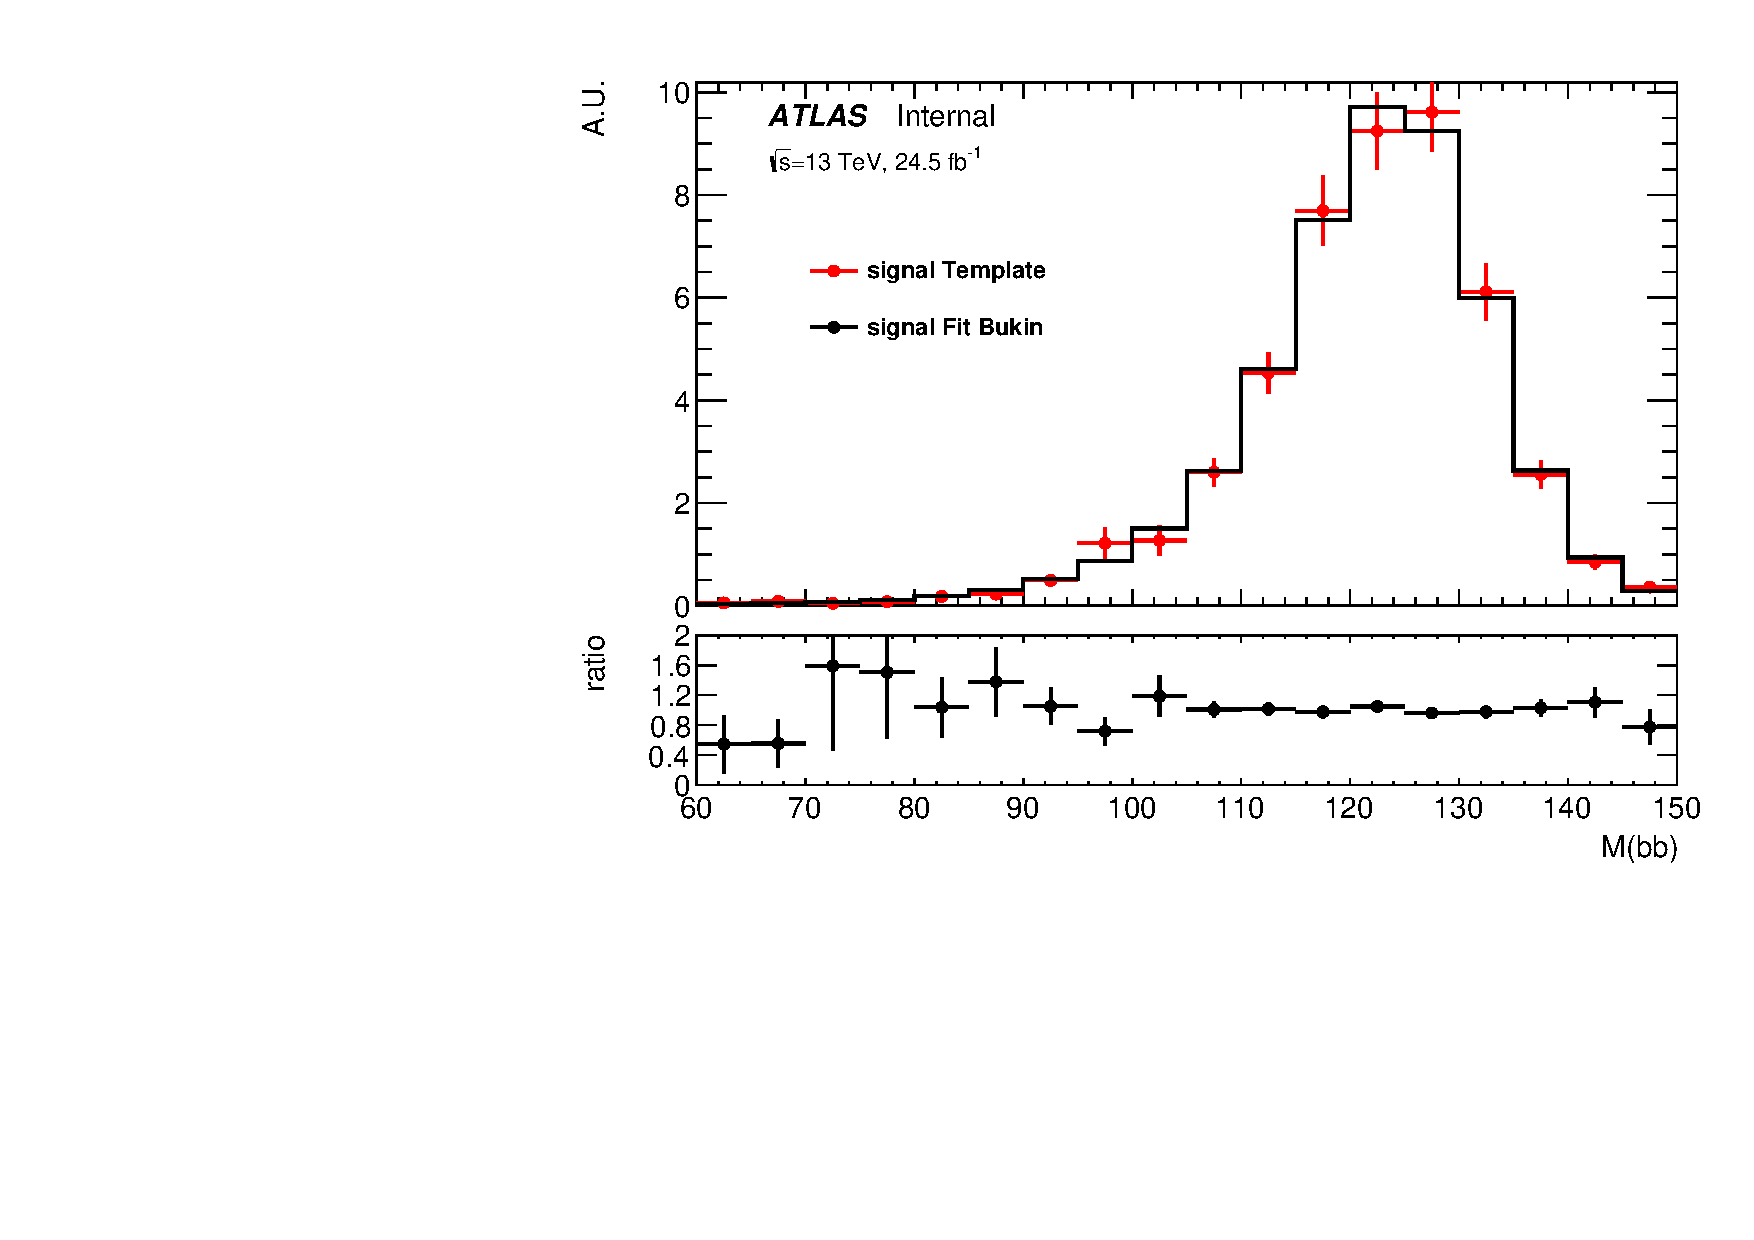
\includegraphics[width=0.32\textwidth]{figures/SigPar/sig_2cen_SRI.pdf}
 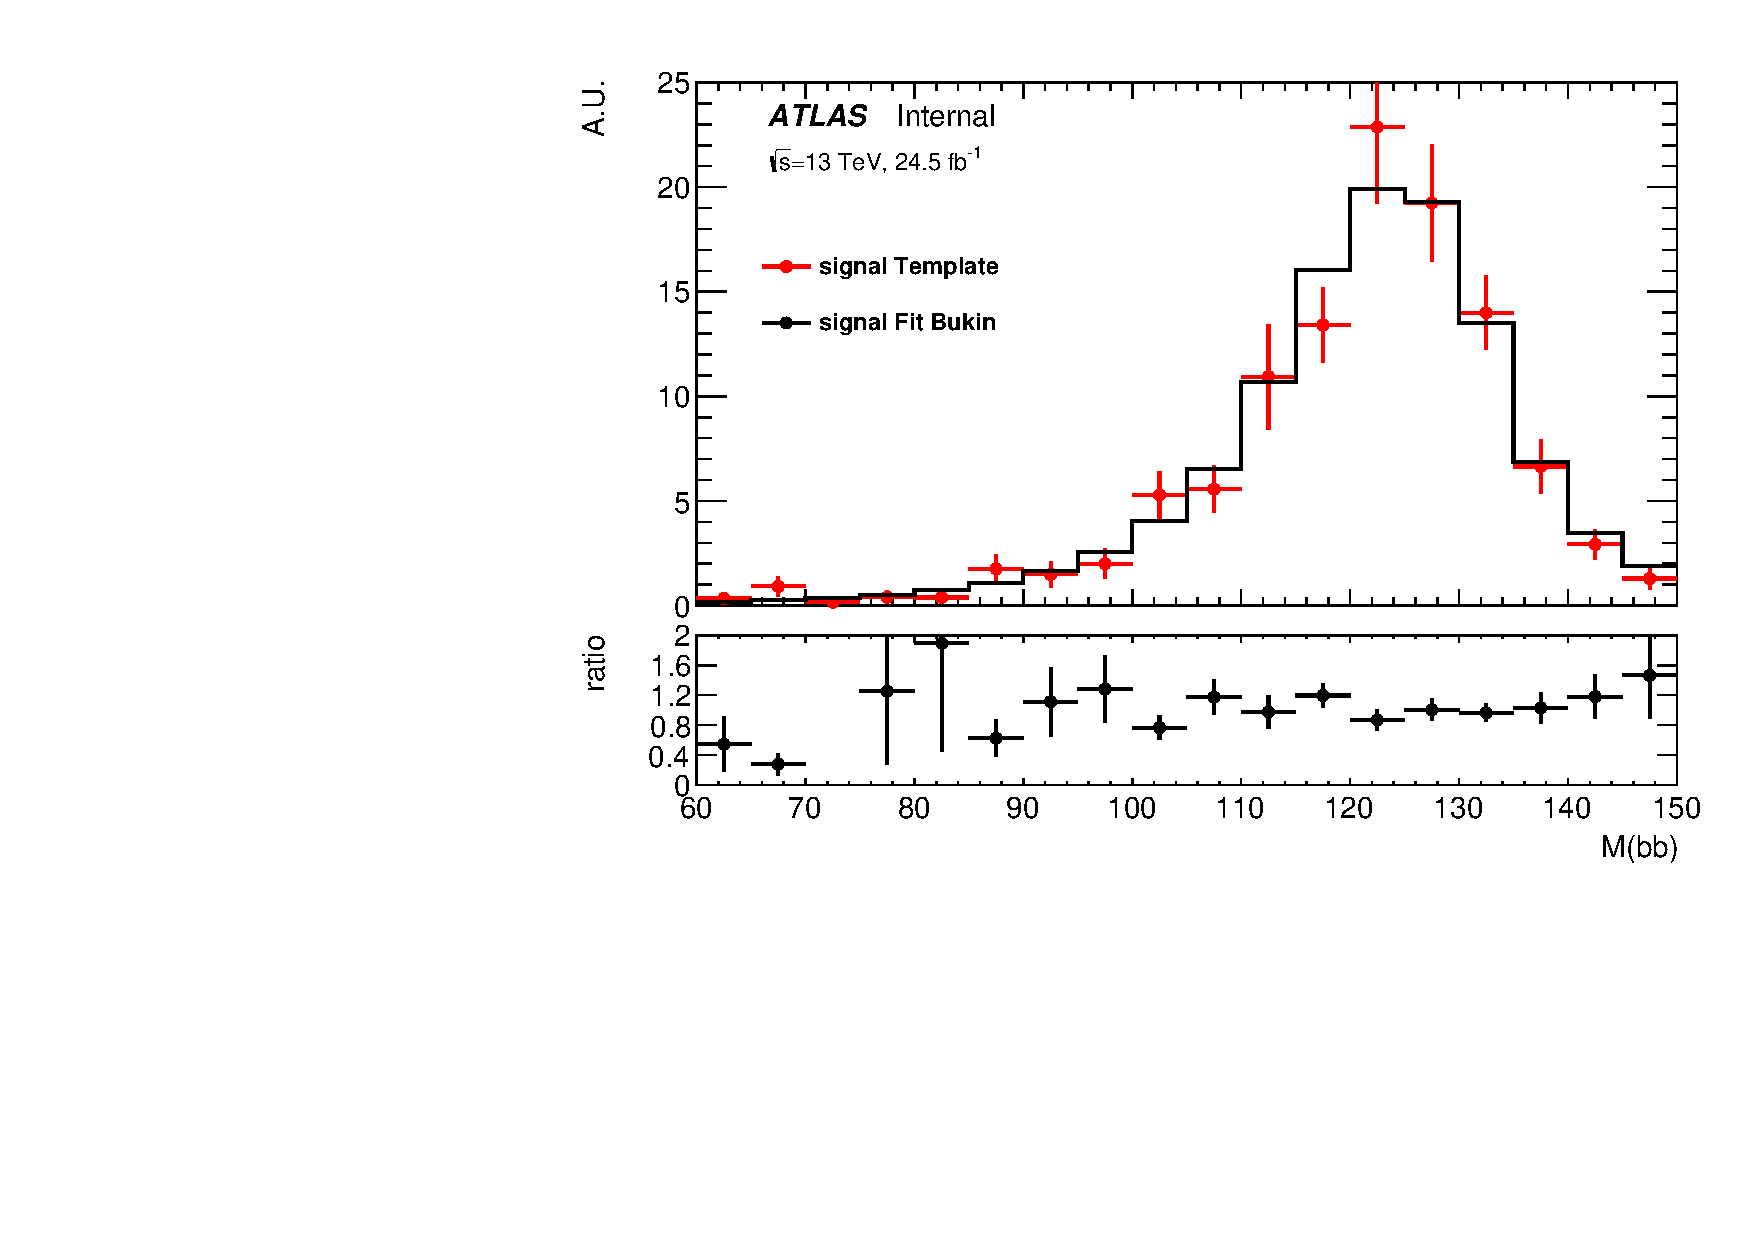
\includegraphics[width=0.32\textwidth]{figures/SigPar/sig_2cen_SRII.pdf}
 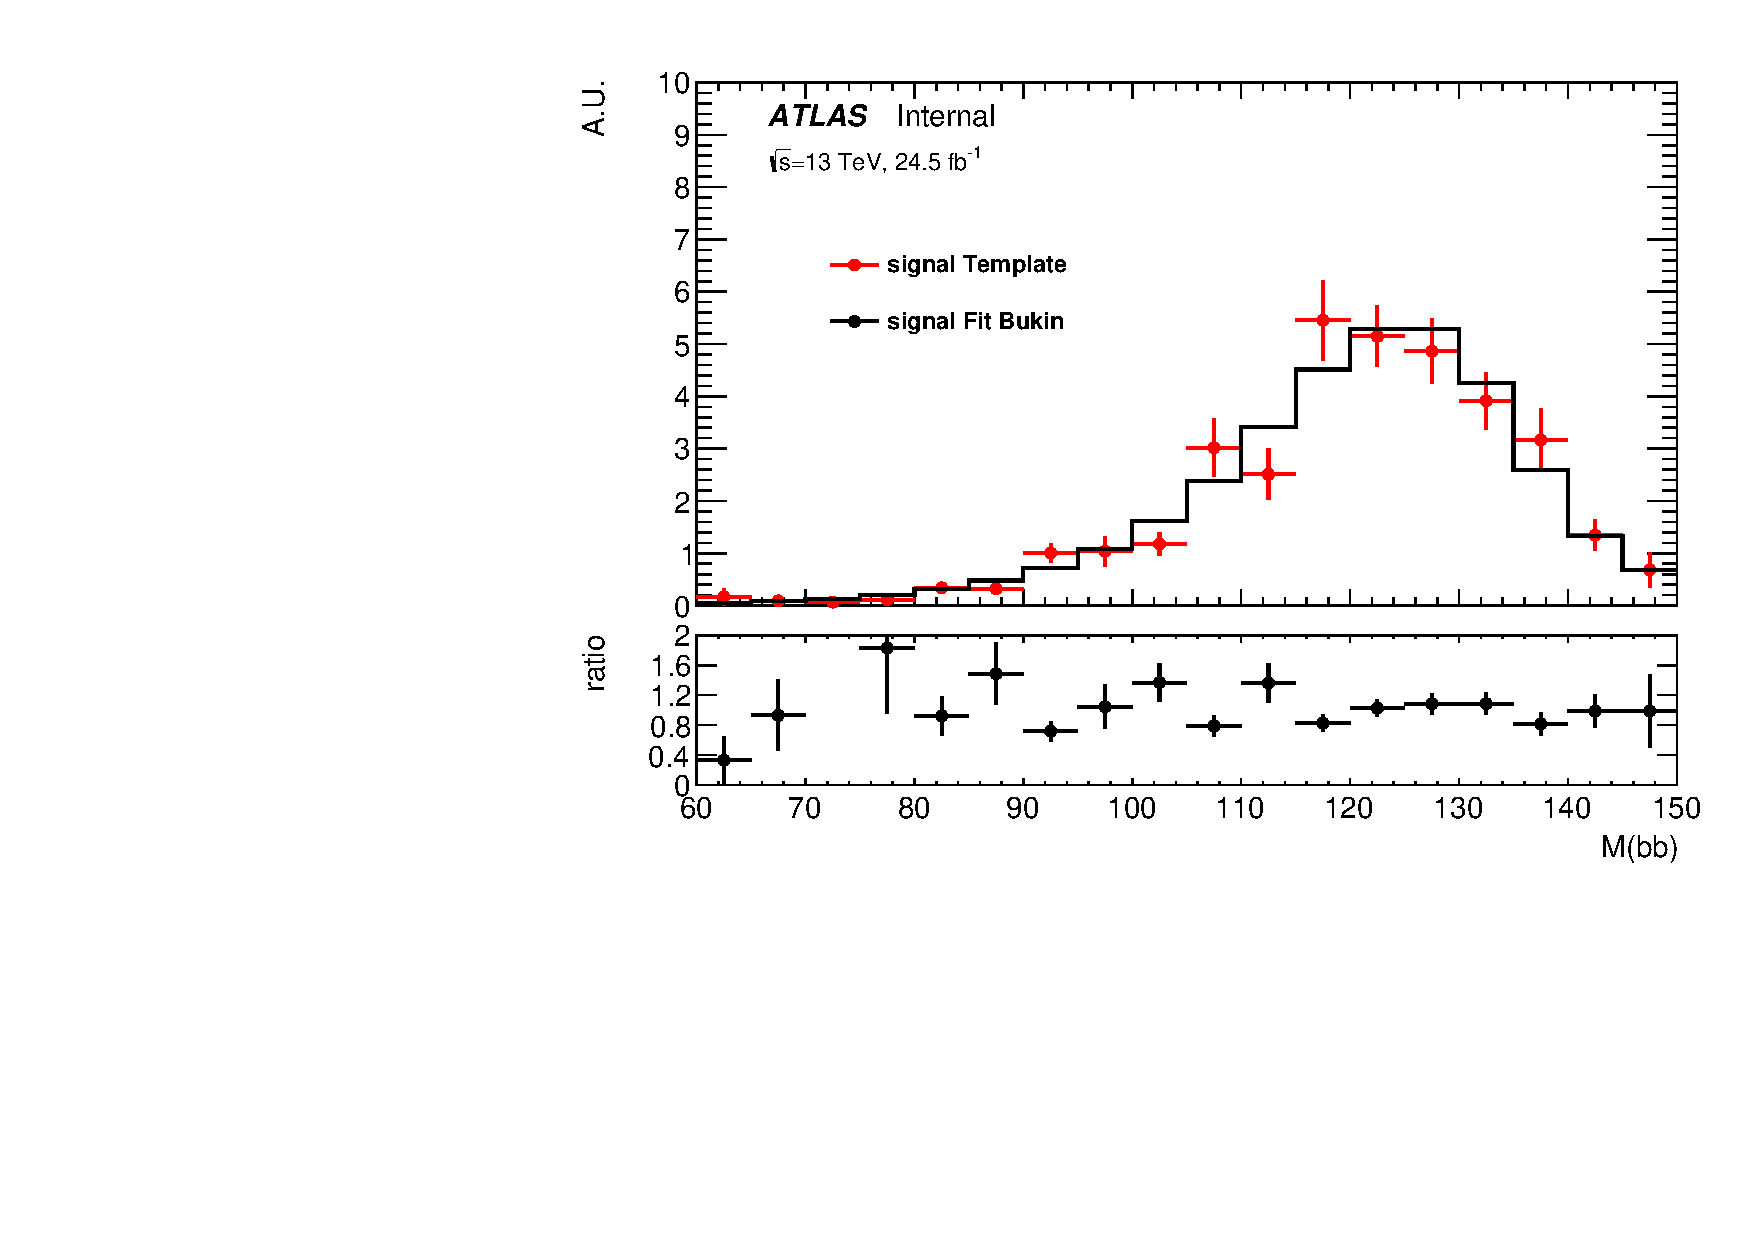
\includegraphics[width=0.32\textwidth]{figures/SigPar/sig_2cen_SRIII.pdf}\\
 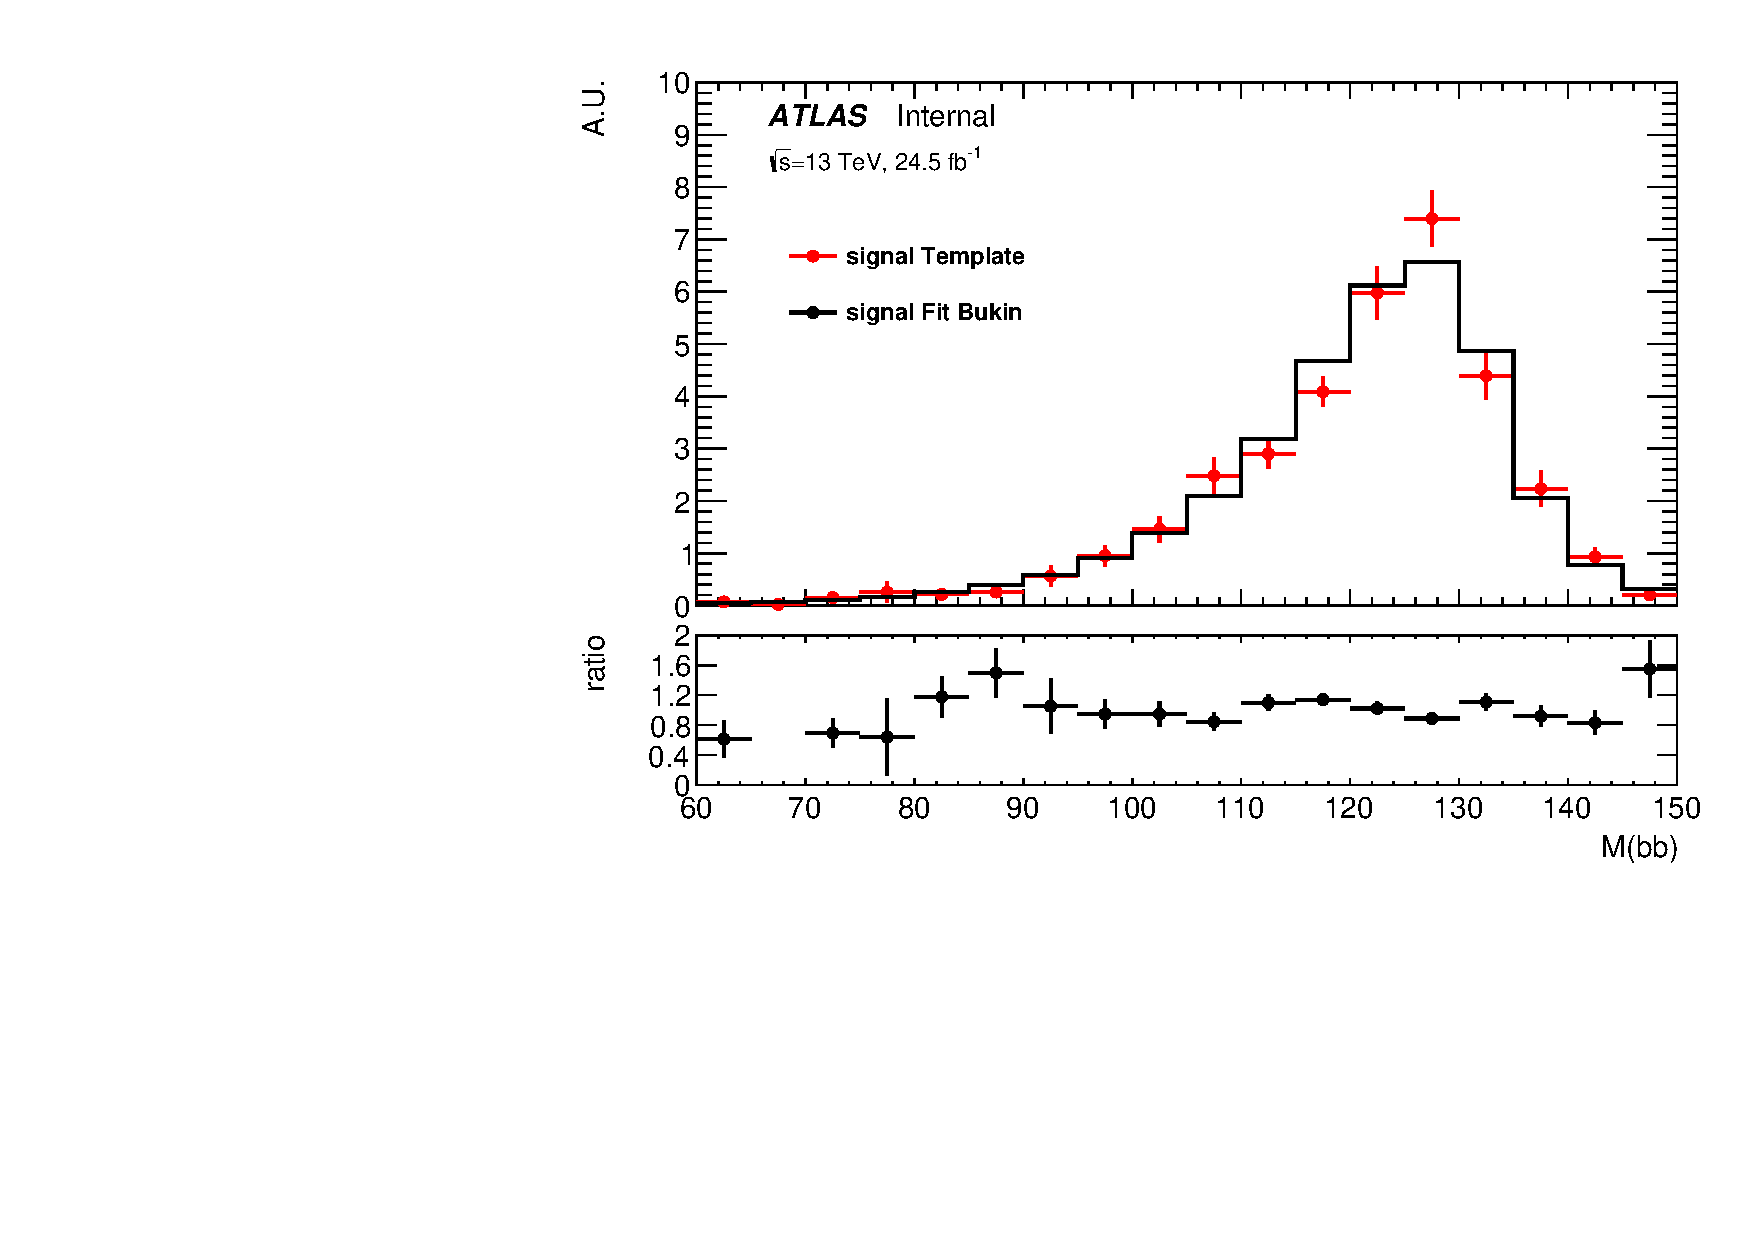
\includegraphics[width=0.32\textwidth]{figures/SigPar/sig_4cen_SRI.pdf}
 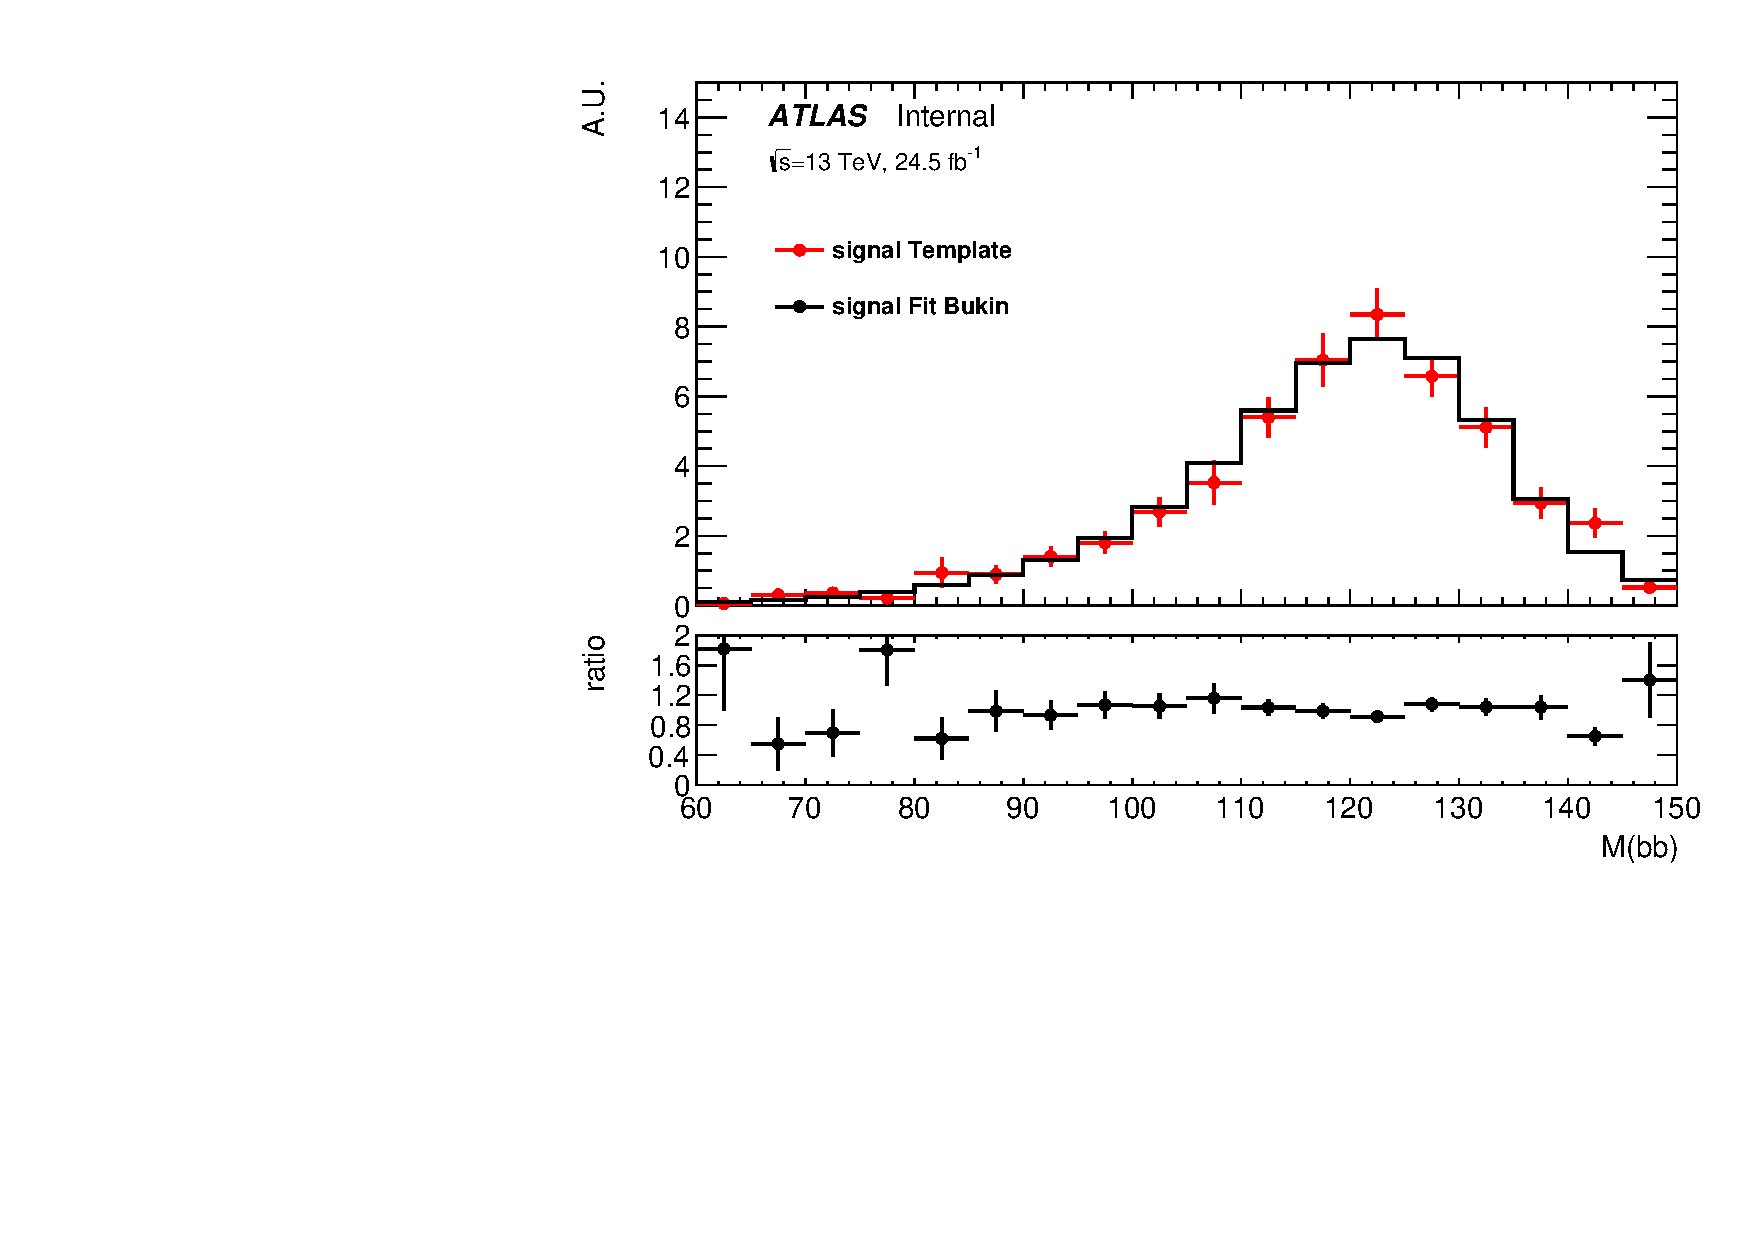
\includegraphics[width=0.32\textwidth]{figures/SigPar/sig_4cen_SRII.pdf}

\caption{Bukin function parametrization of signal \Mbb{} distribution in SR I - SR III of \twocentral (top) and SR I - SR II of \fourcentral (bottom)}
  \label{fig:sigpar-old}
\end{figure}


\begin{figure}[htbp]
  \centering    
 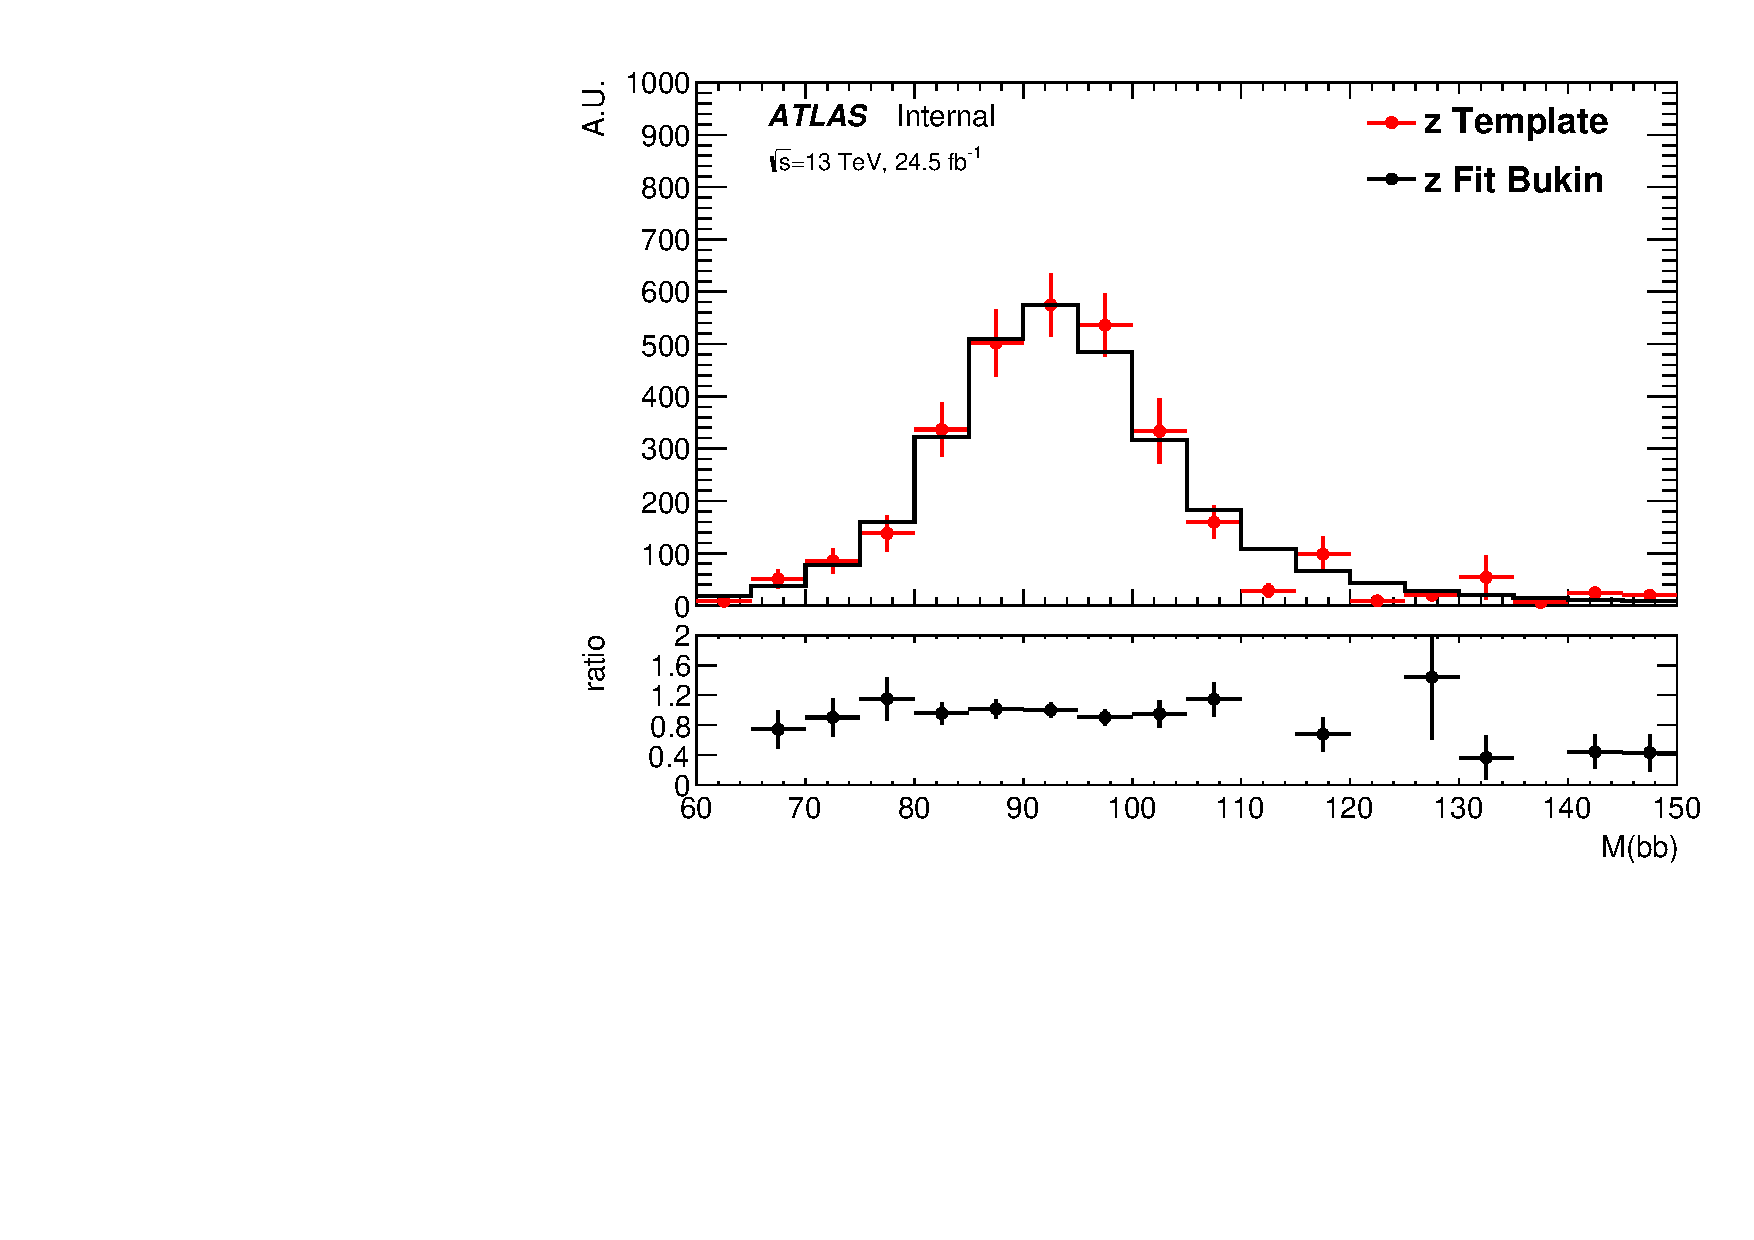
\includegraphics[width=0.45\textwidth]{figures/SigPar/z_2cen.pdf}
 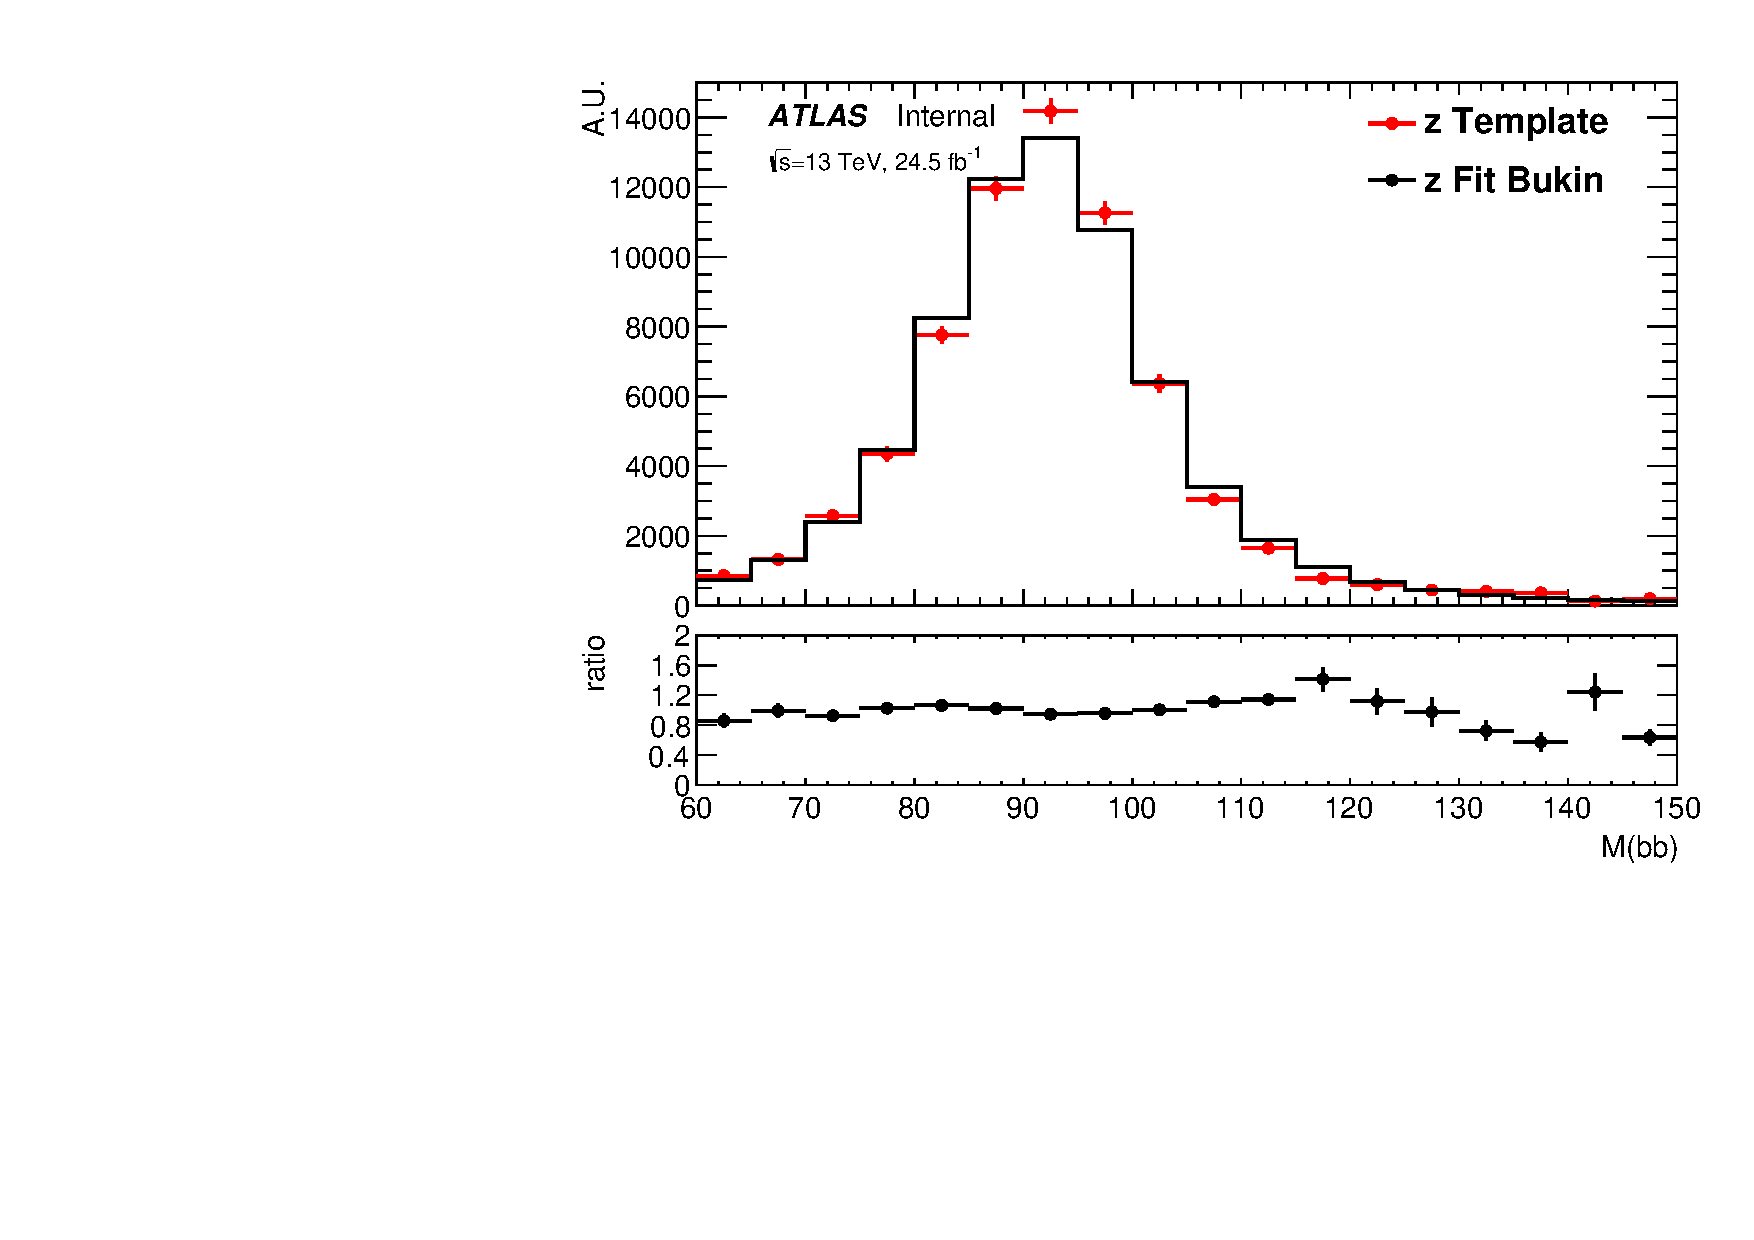
\includegraphics[width=0.45\textwidth]{figures/SigPar/z_4cen.pdf}

\caption{Bukin function parametrization of \zjets~\Mbb{} distribution in \twocentral (left) and \fourcentral (right)}
  \label{fig:zpar-old}
\end{figure}


\begin{table}[]
\centering
\caption{Goodness of fit for the Bukin parametertizationns and signal and \zjets{} \Mbb{} distributions.}
\label{tab:sigpar-old}
\begin{tabular}{|l|l|l|l|}
\hline
Process  & Signal \twocentral SR I  & Signal \twocentral SR II  & Signal \twocentral SR III \\ \hline
$\chi^2$ ($\chi^2$ prob) & 1.27 (0.21)                     & 0.79 (0.70)                      & 0.54 (0.93)                      \\ \hline
Process  & Signal \fourcentral SR I & Signal \fourcentral SR II &                           \\ \hline
$\chi^2$ ($\chi^2$ prob) & 0.74 (0.75)                     & 1.14 (0.31)                      &                           \\ \hline
Process  & \zjets \twocentral       & \zjets \fourcentral       &                           \\ \hline
$\chi^2$ ($\chi^2$ prob) & 1.7 (0.04)                      & 1.32 (0.17)                      &                           \\ \hline
\end{tabular}
\end{table}


\subsubsection{Non-resonant \Mbb{} distribution}
\label{sec:nonres-old}

Given that the BDT discriminant is not highly correlated with \Mbb{}, the shape of the non-resonant distribution does not change significantly between
control and signal regions.  We hypothesize that the difference between the shapes in the various regions can be described by a linear transfer function.  
Figures~\ref{fig:mbb_2tag_2cen-old}~and~\ref{fig:mbb_2tag_4cen-old} and 
Tables~\ref{tab:mbb_lin_2cen-old}~and~\ref{tab:mbb_lin_4cen-old} show that the ratios
 between each region are compatible with a linear fit. 
Therefore,  the profile likelihood assumes that the shape for the non-resonant background
is the same in all regions up to a linear correction. The function parameters are therefore
shared across all regions except for two coefficients specific to each region, reducing the total number of function parameters from 28 to 18.

\begin{figure}[htbp]
  \centering
 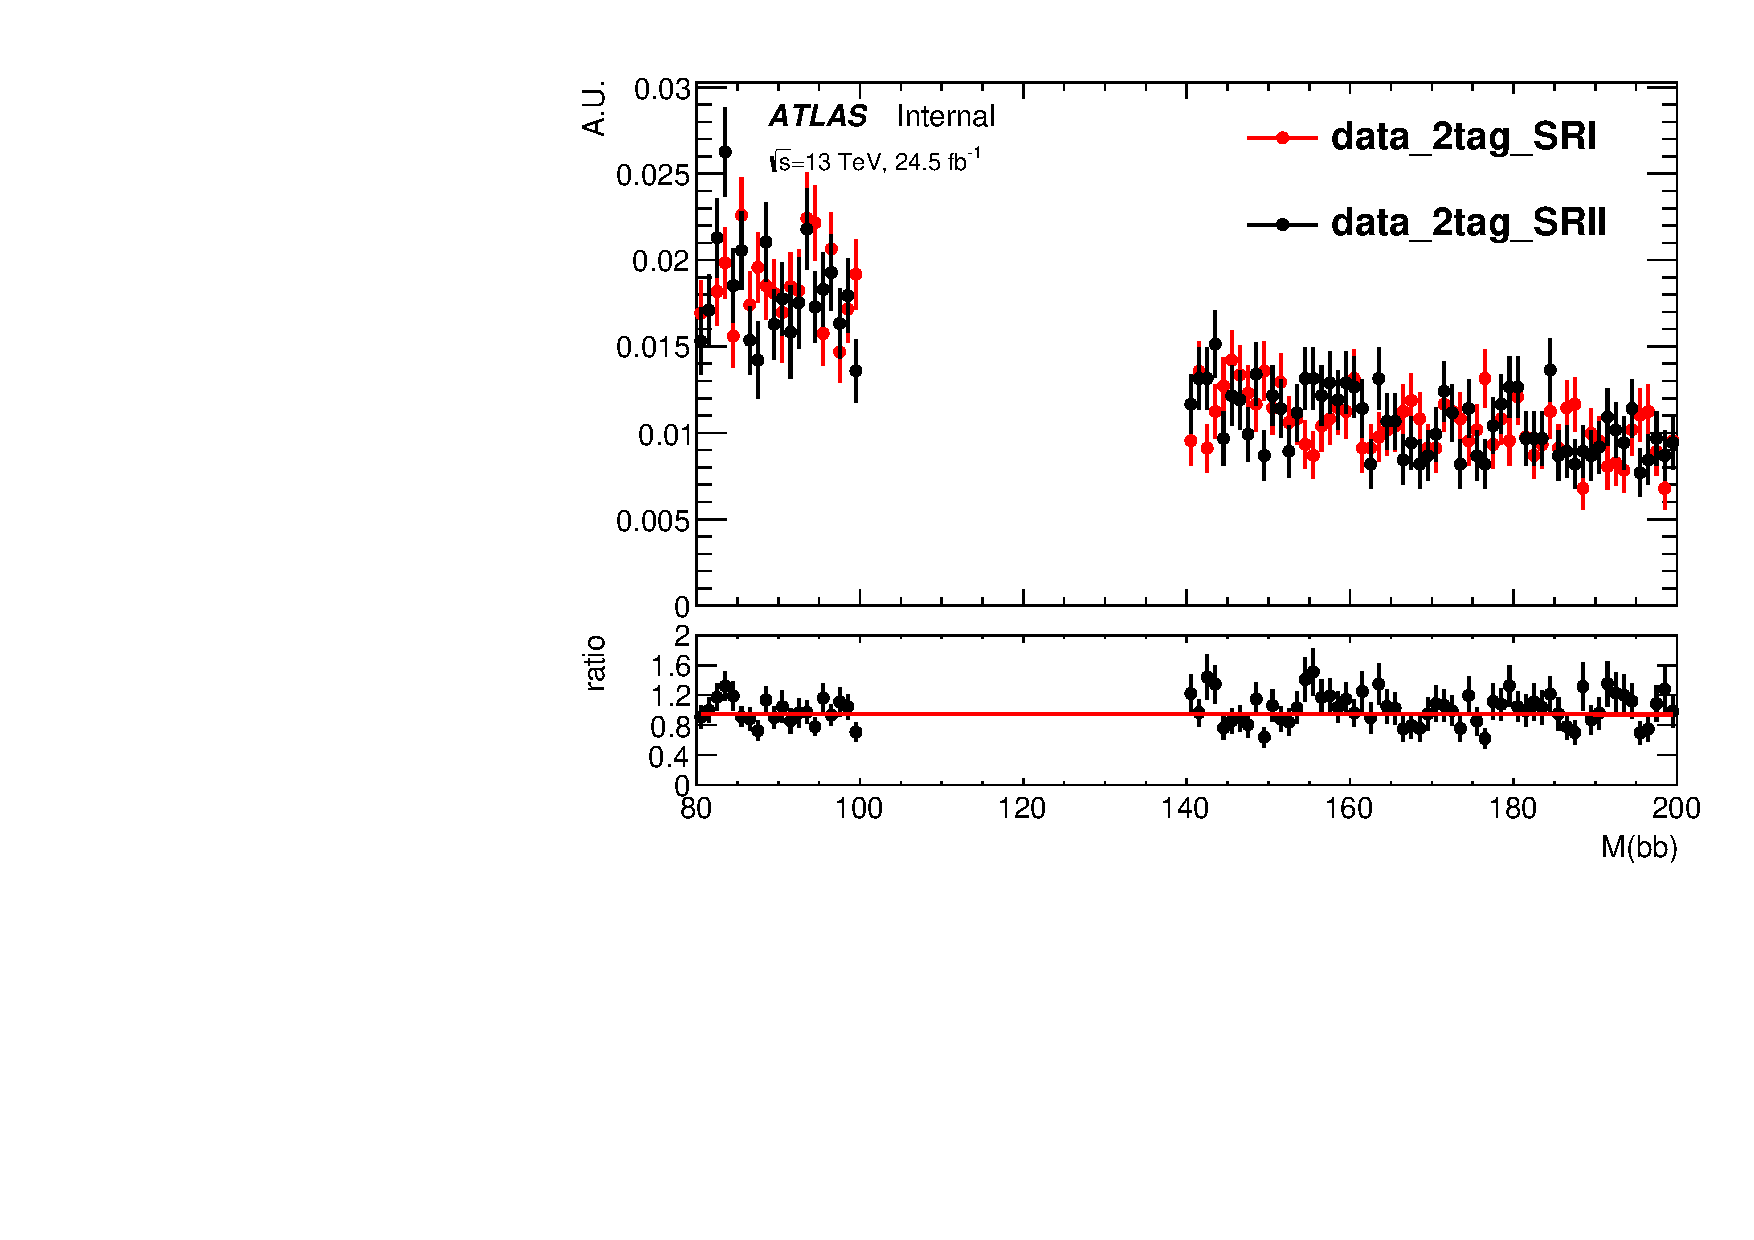
\includegraphics[width=0.45\textwidth]{figures/Mbb_SRI_SRII_2cen.pdf}
 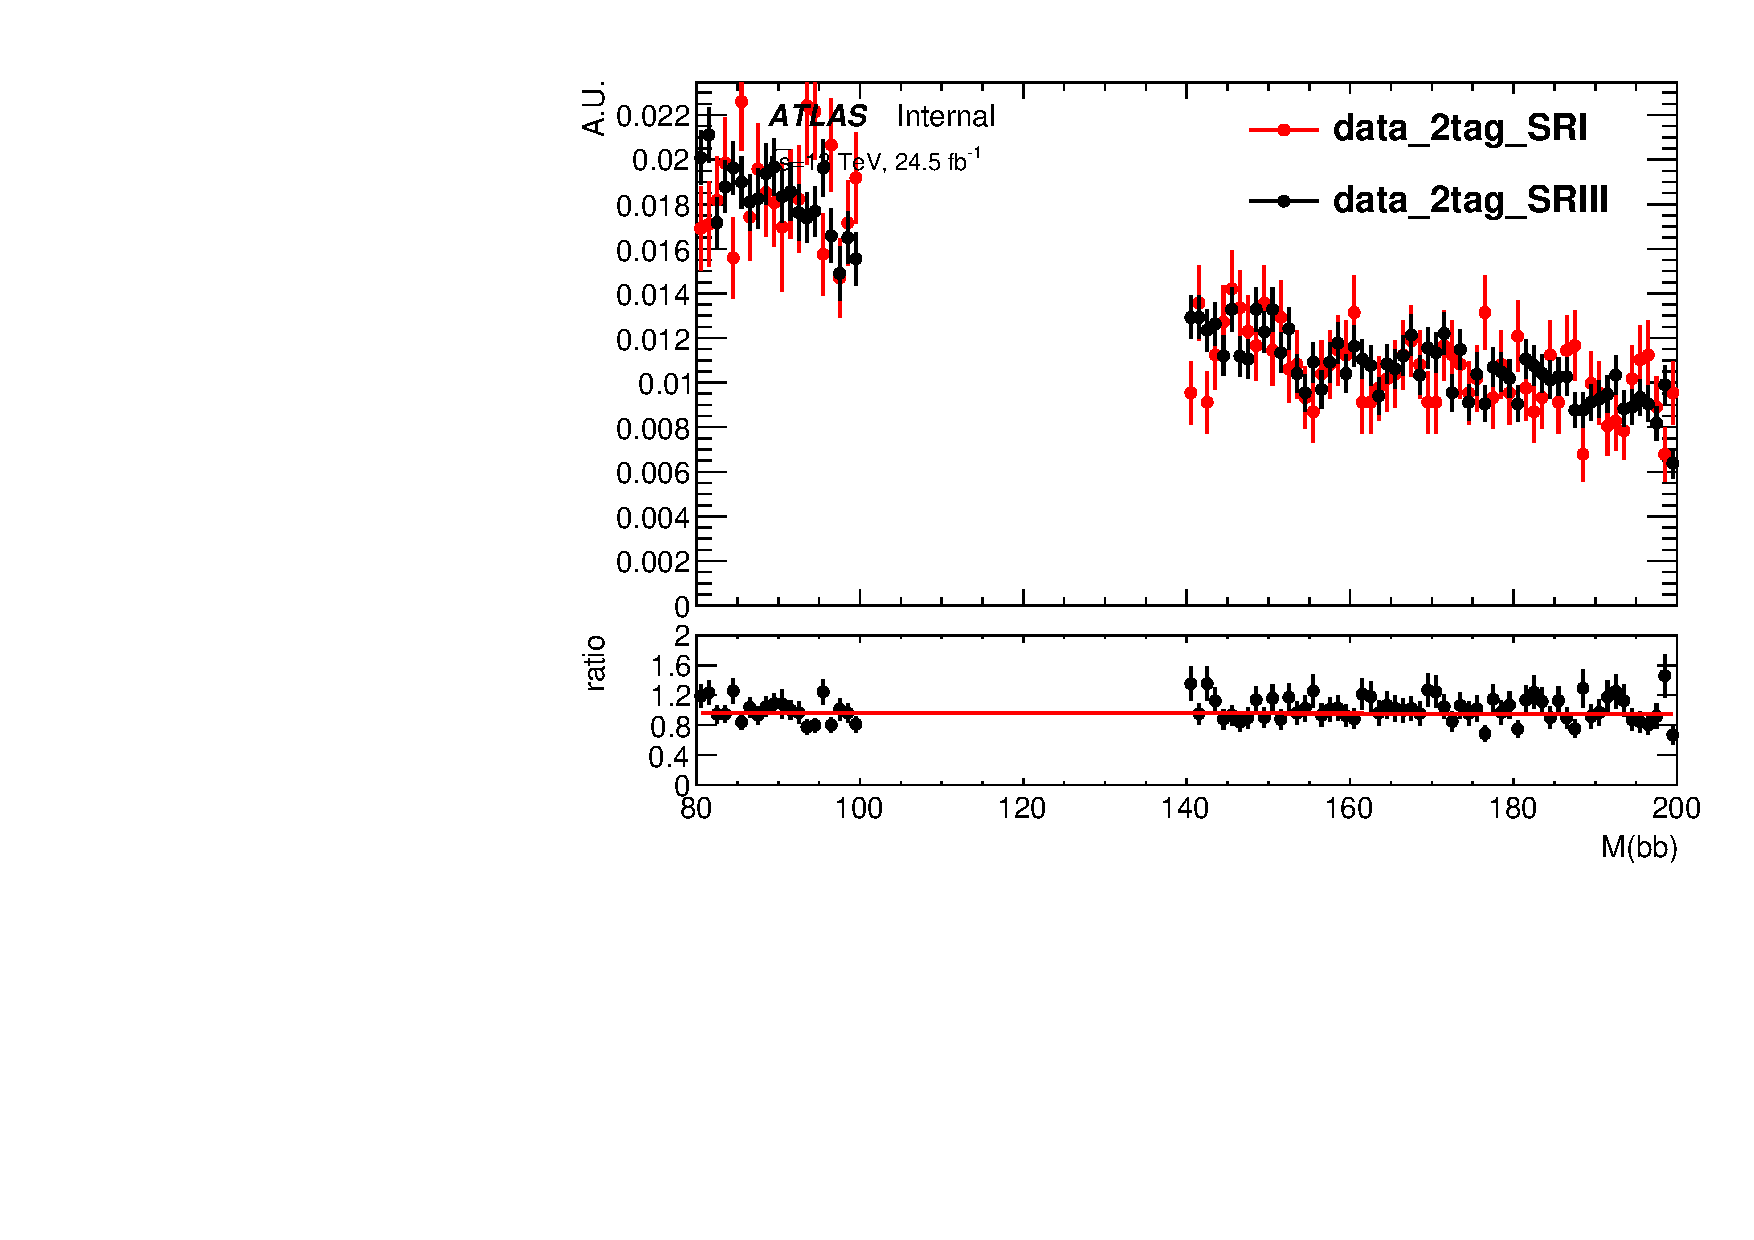
\includegraphics[width=0.45\textwidth]{figures/Mbb_SRI_SRIII_2cen.pdf}\\
 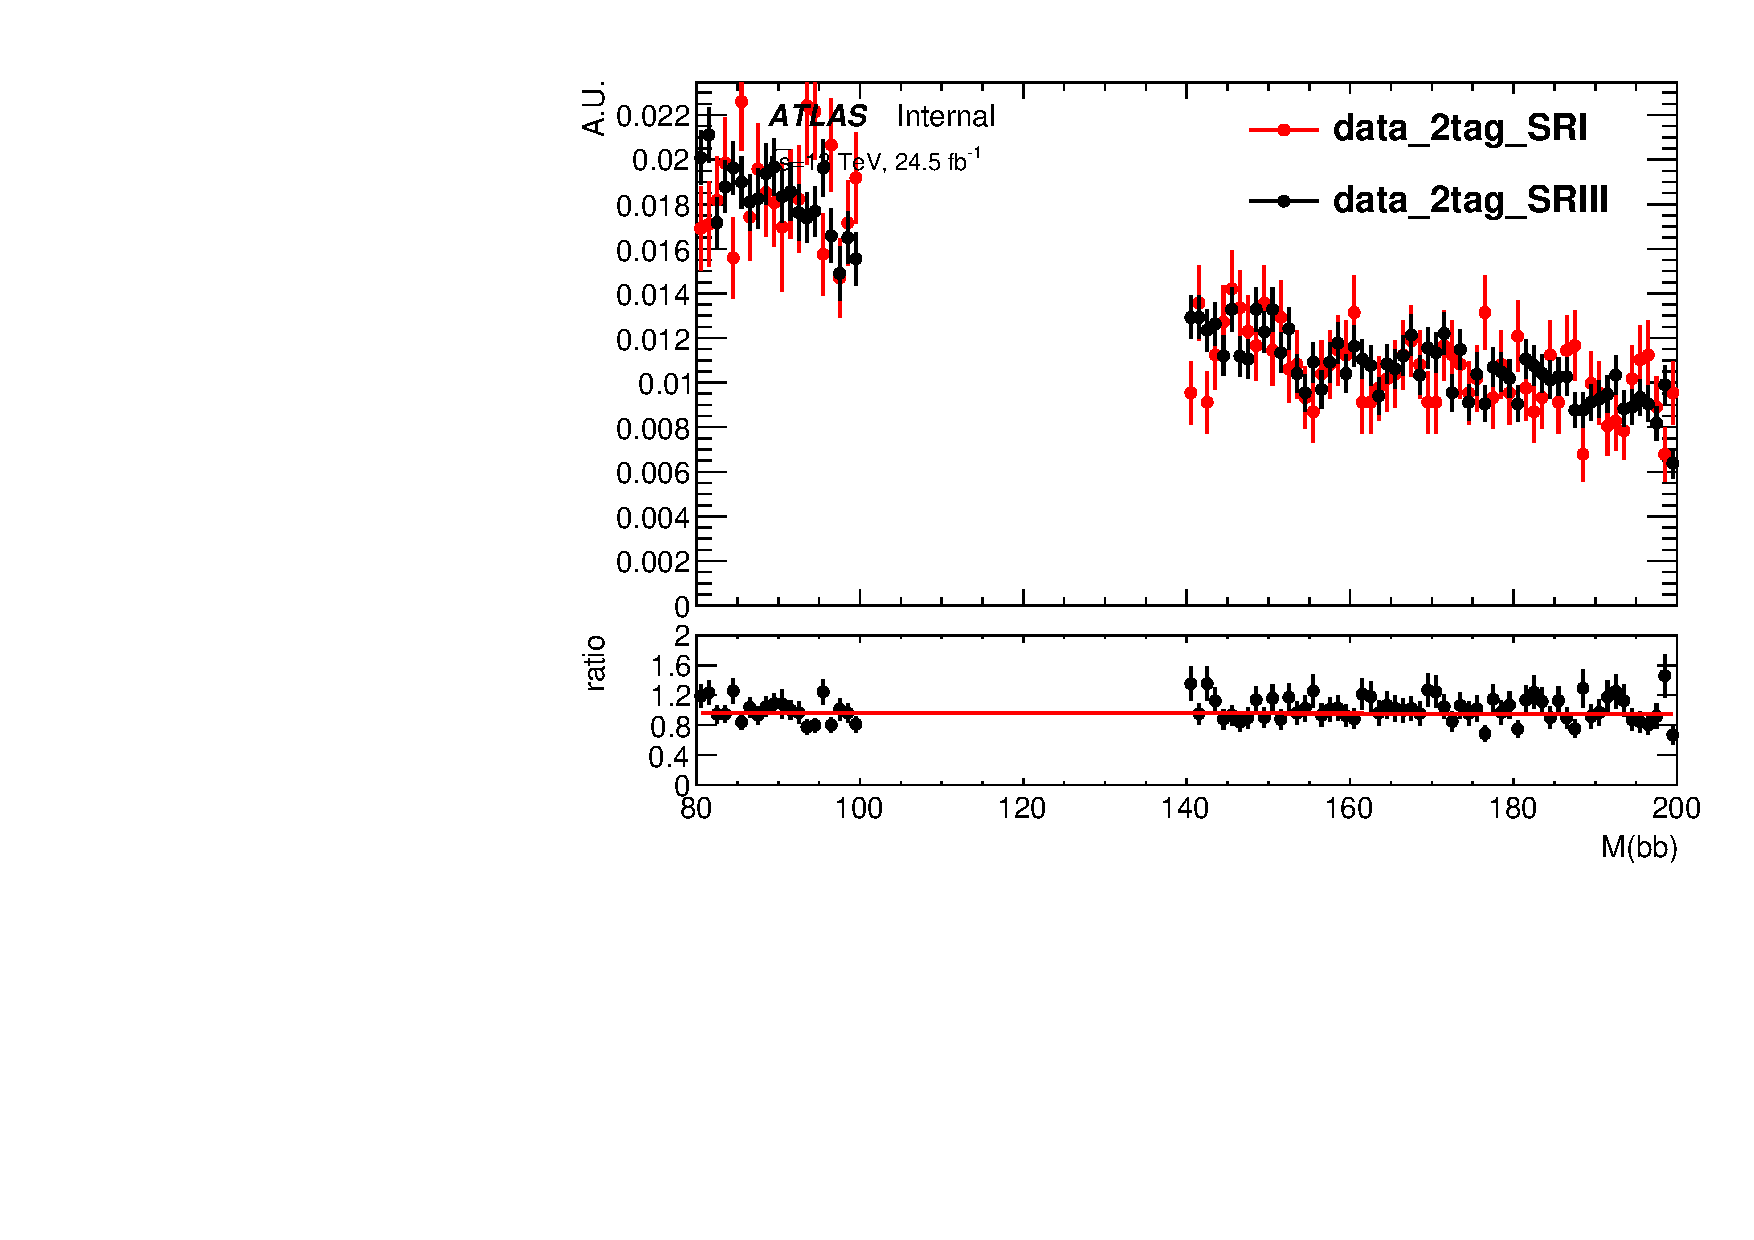
\includegraphics[width=0.45\textwidth]{figures/Mbb_SRI_SRIII_2cen.pdf}
 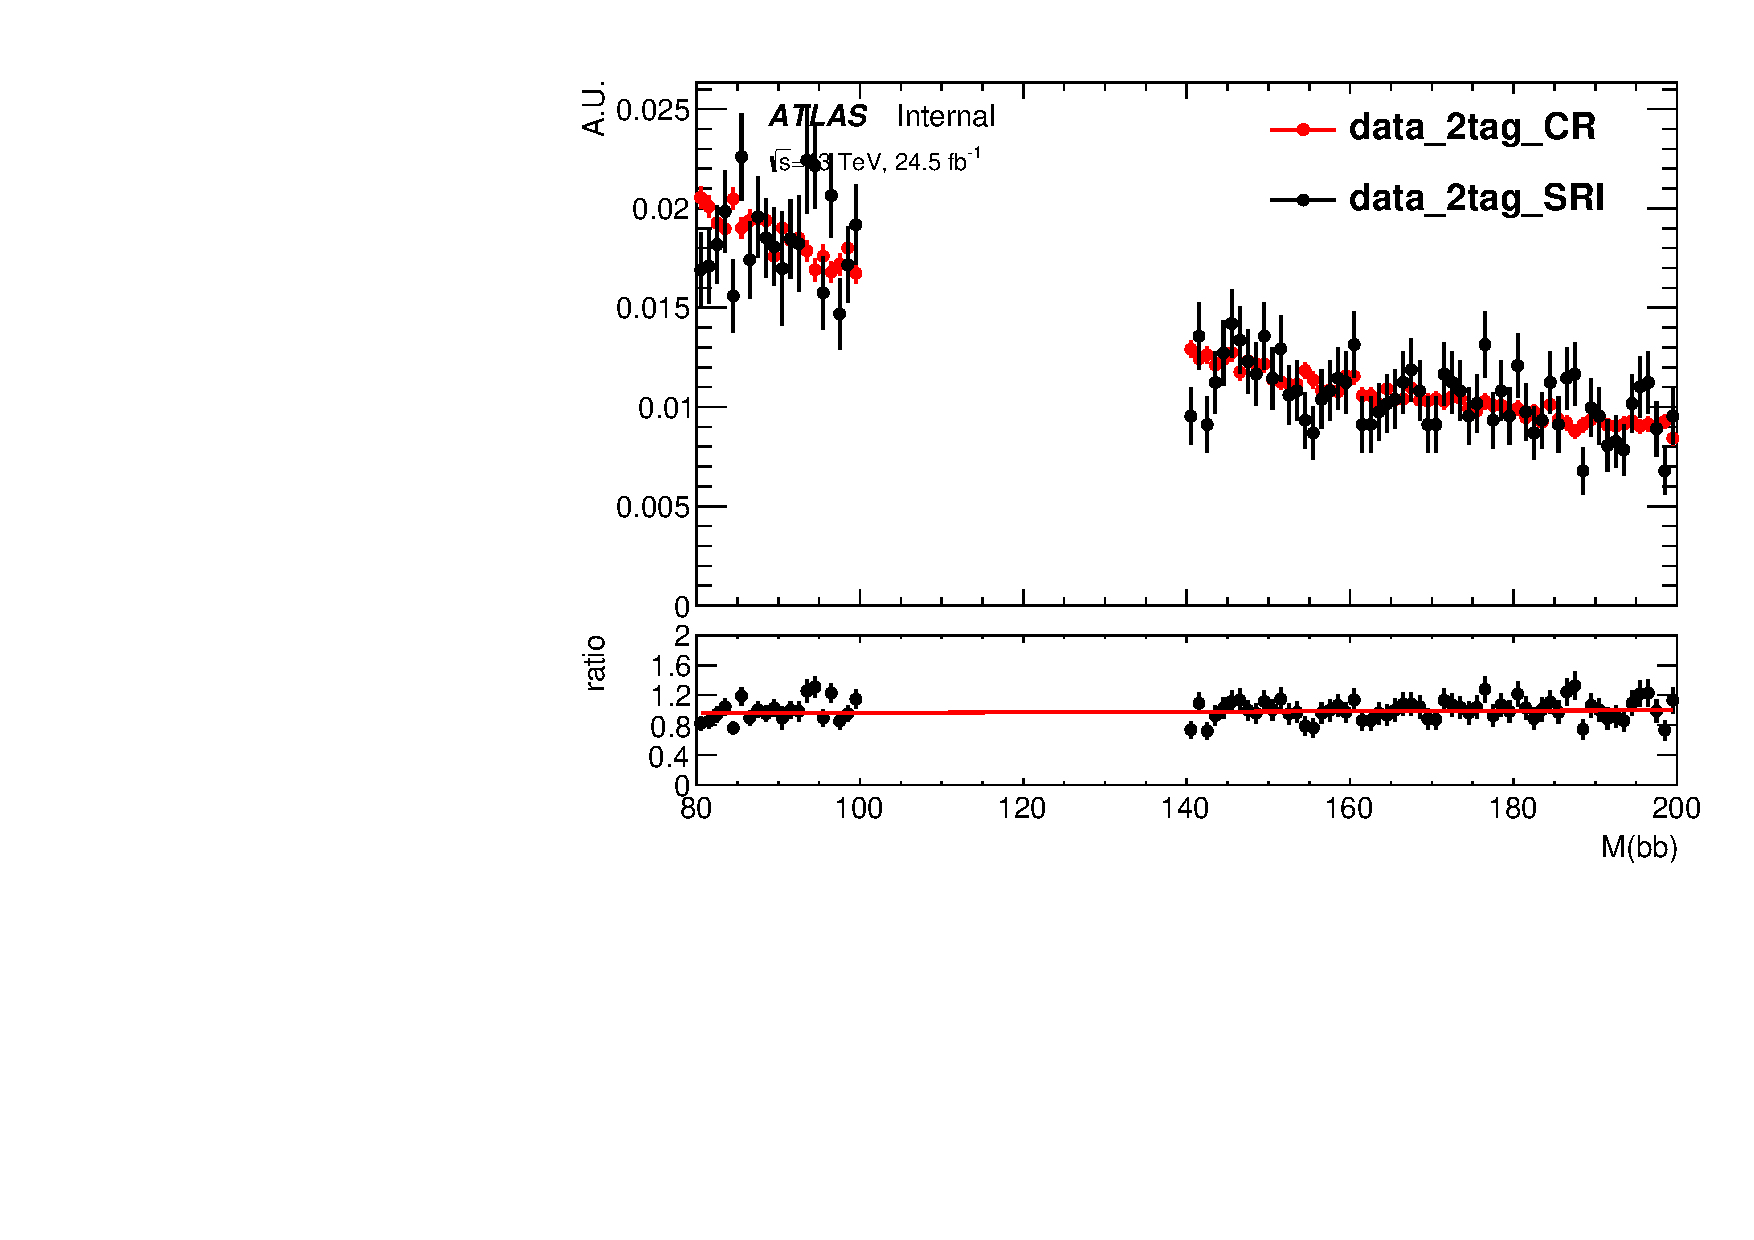
\includegraphics[width=0.45\textwidth]{figures/Mbb_CR_SRI_2cen.pdf}\\
 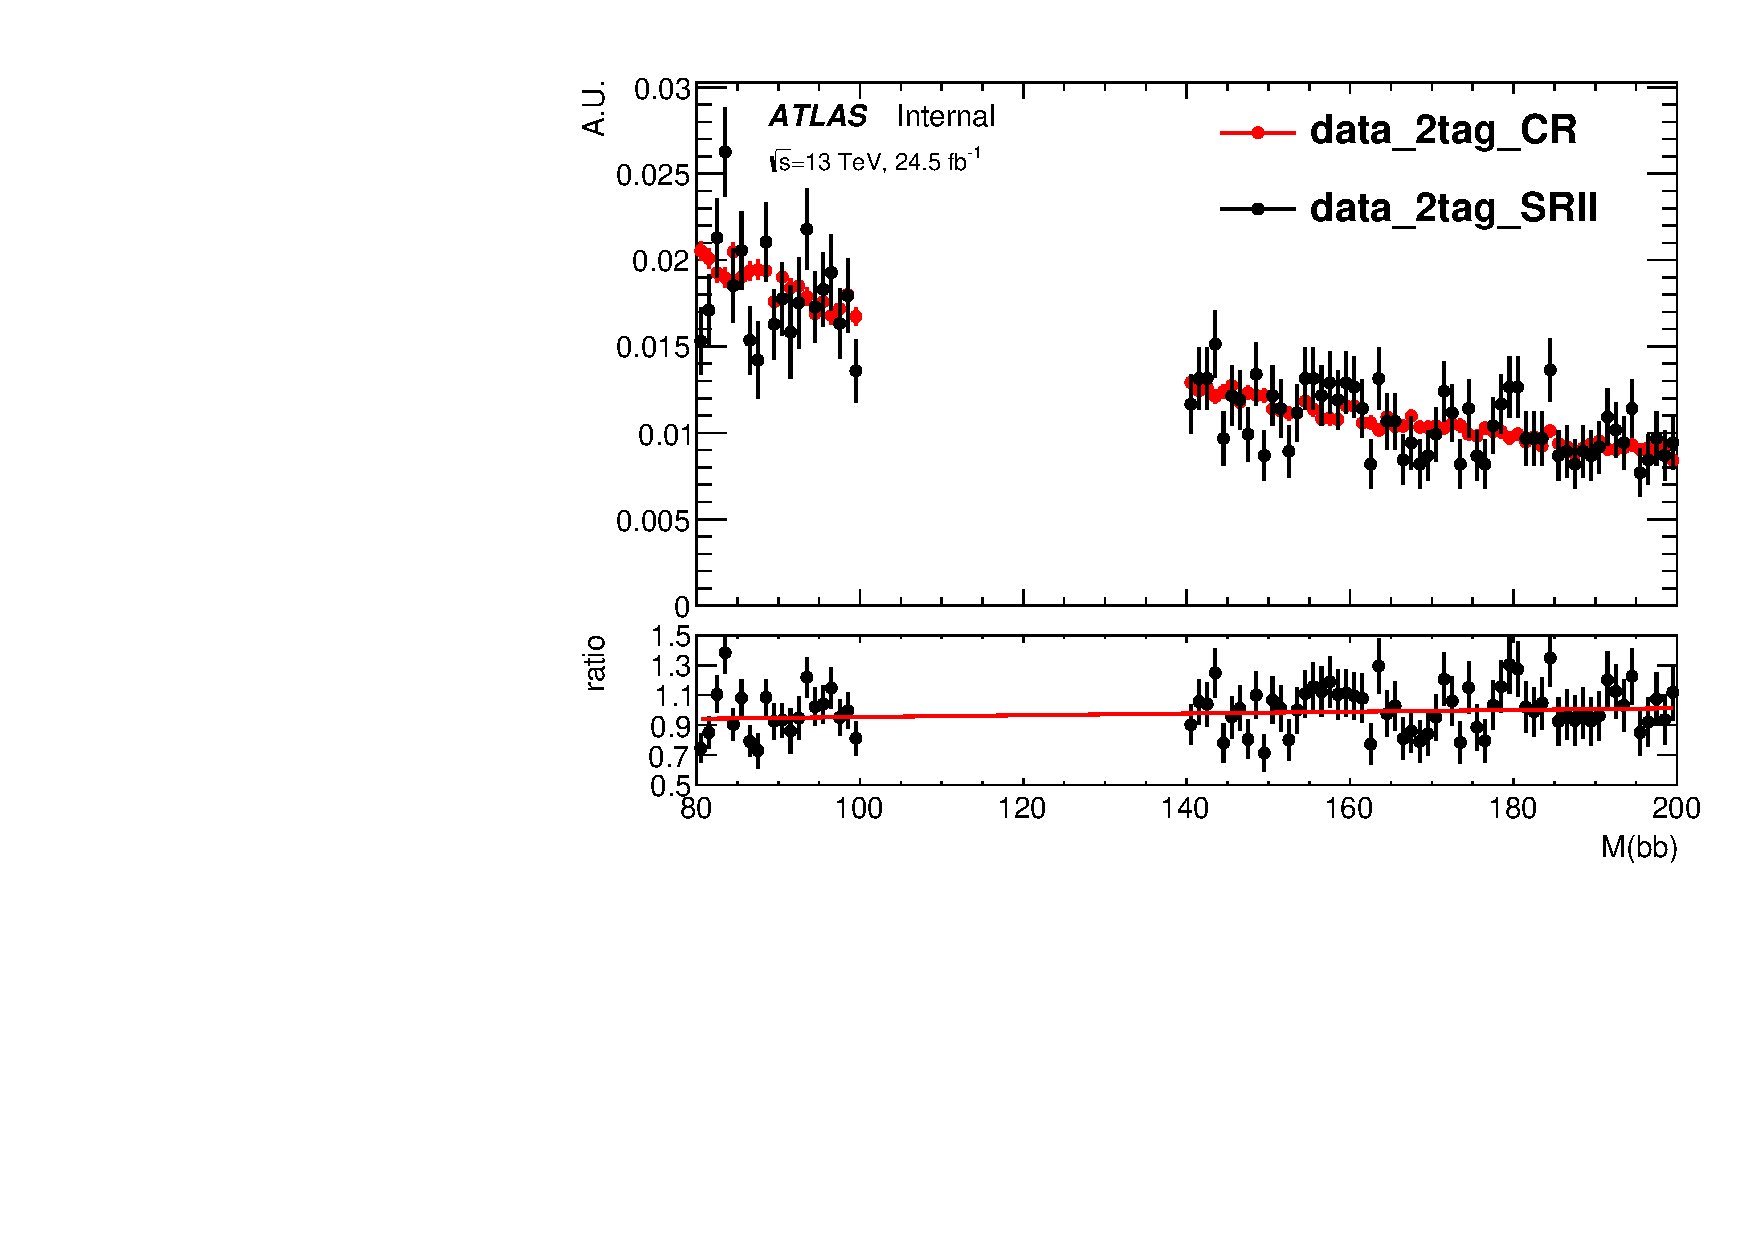
\includegraphics[width=0.45\textwidth]{figures/Mbb_CR_SRII_2cen.pdf}
 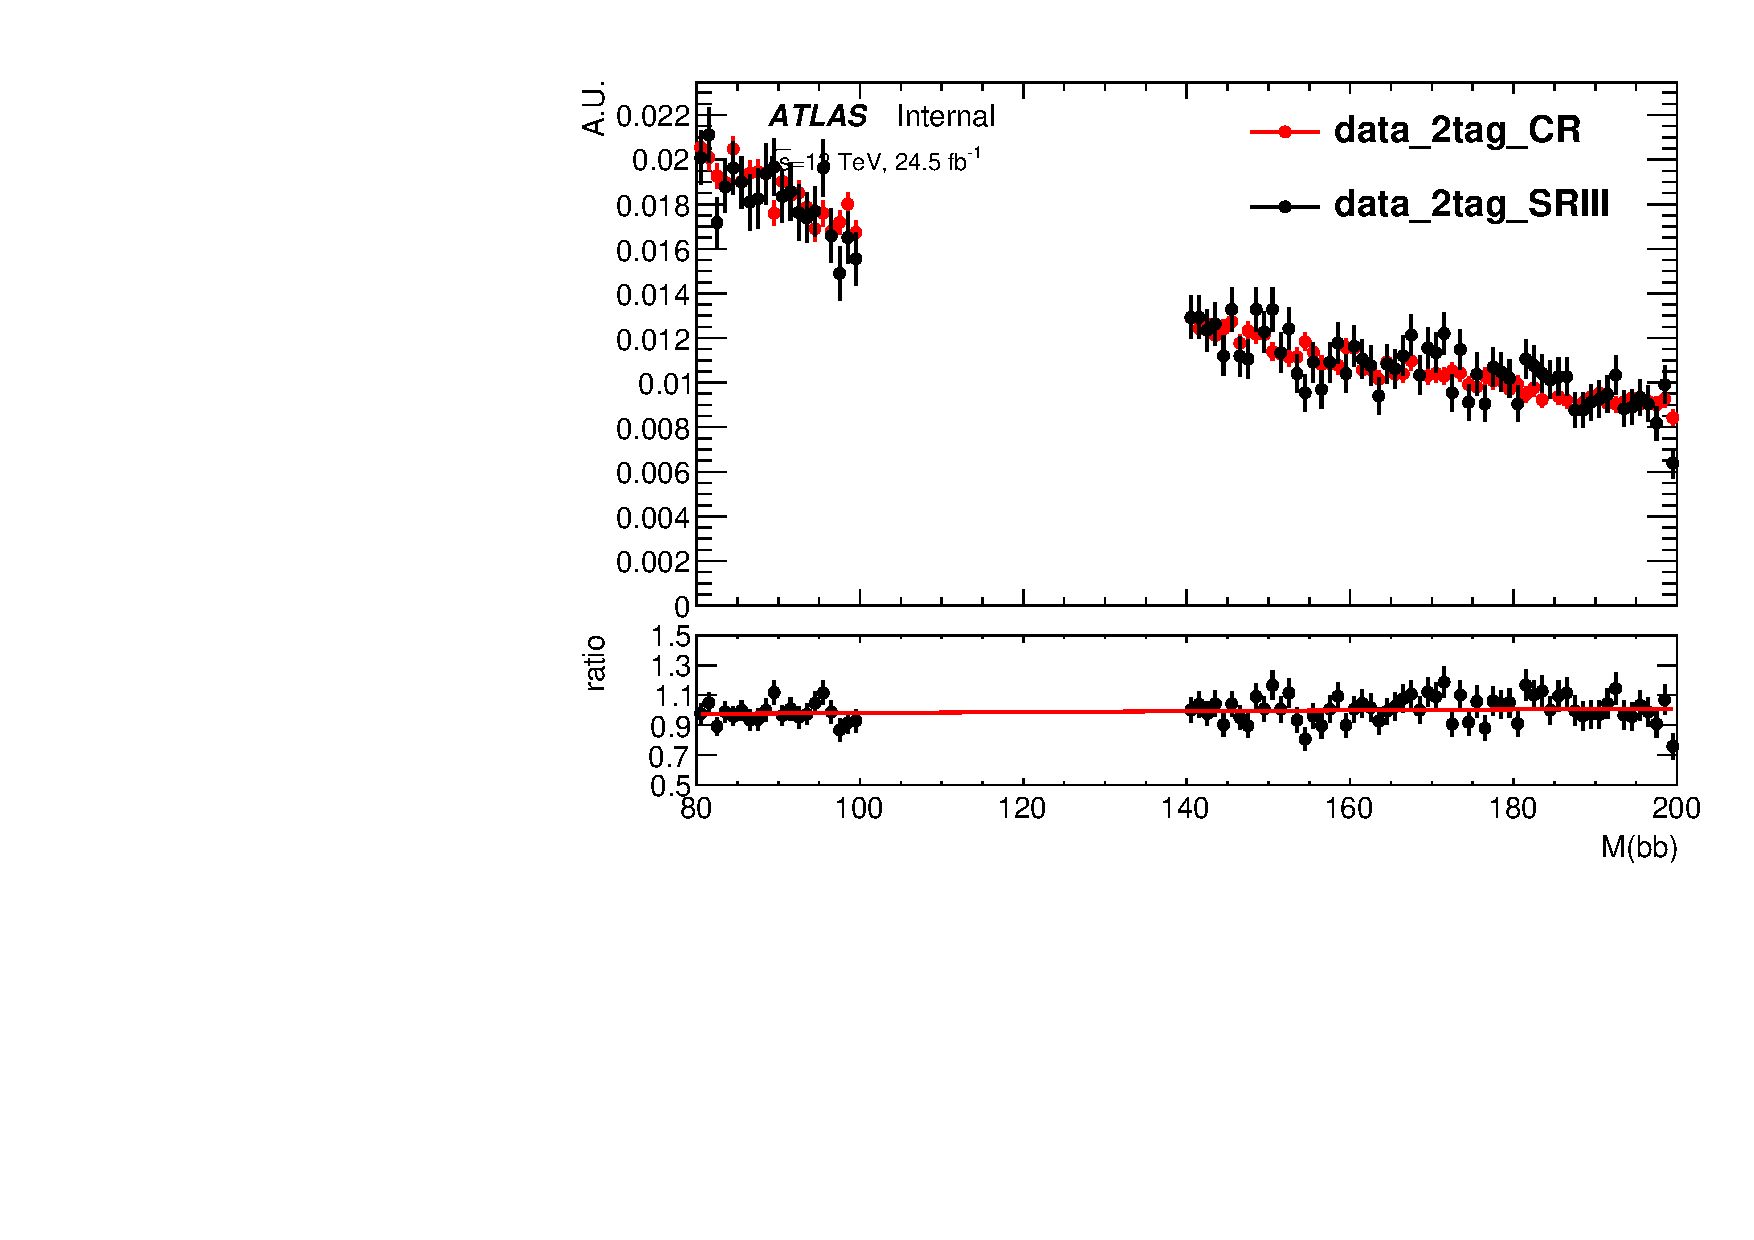
\includegraphics[width=0.45\textwidth]{figures/Mbb_CR_SRIII_2cen.pdf}\\

\caption{\Mbb~shape comparison between CR and both SR for the \twocentral channel.  The bottom panel in each plot shows the ratio of the two plotted distributions. The $\chi^2$/ndof of the linear fits are reported in Table~\ref{tab:mbb_lin_2cen-old}.}
  \label{fig:mbb_2tag_2cen-old}
\end{figure}

\begin{figure}[htbp]
  \centering
 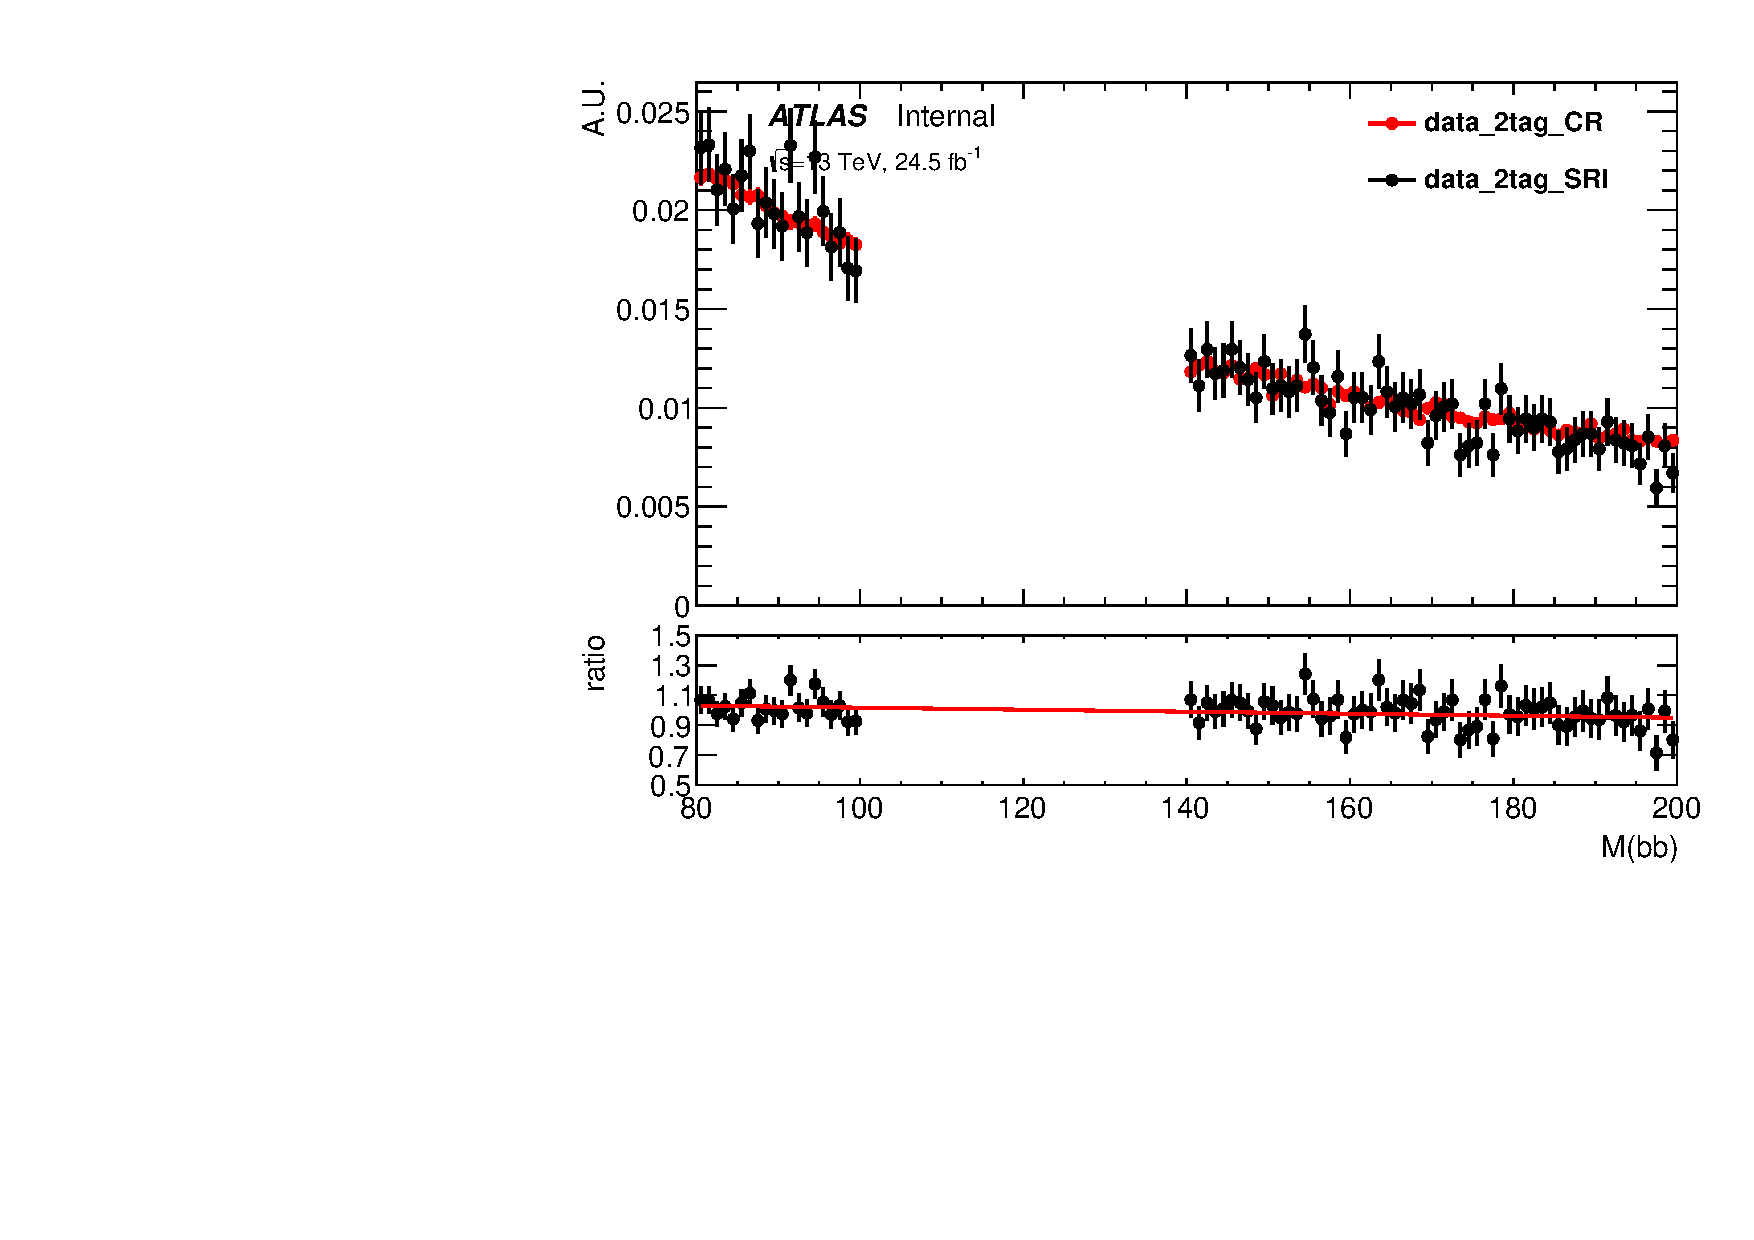
\includegraphics[width=0.45\textwidth]{figures/Mbb_CR_SRI_4cen.pdf}
 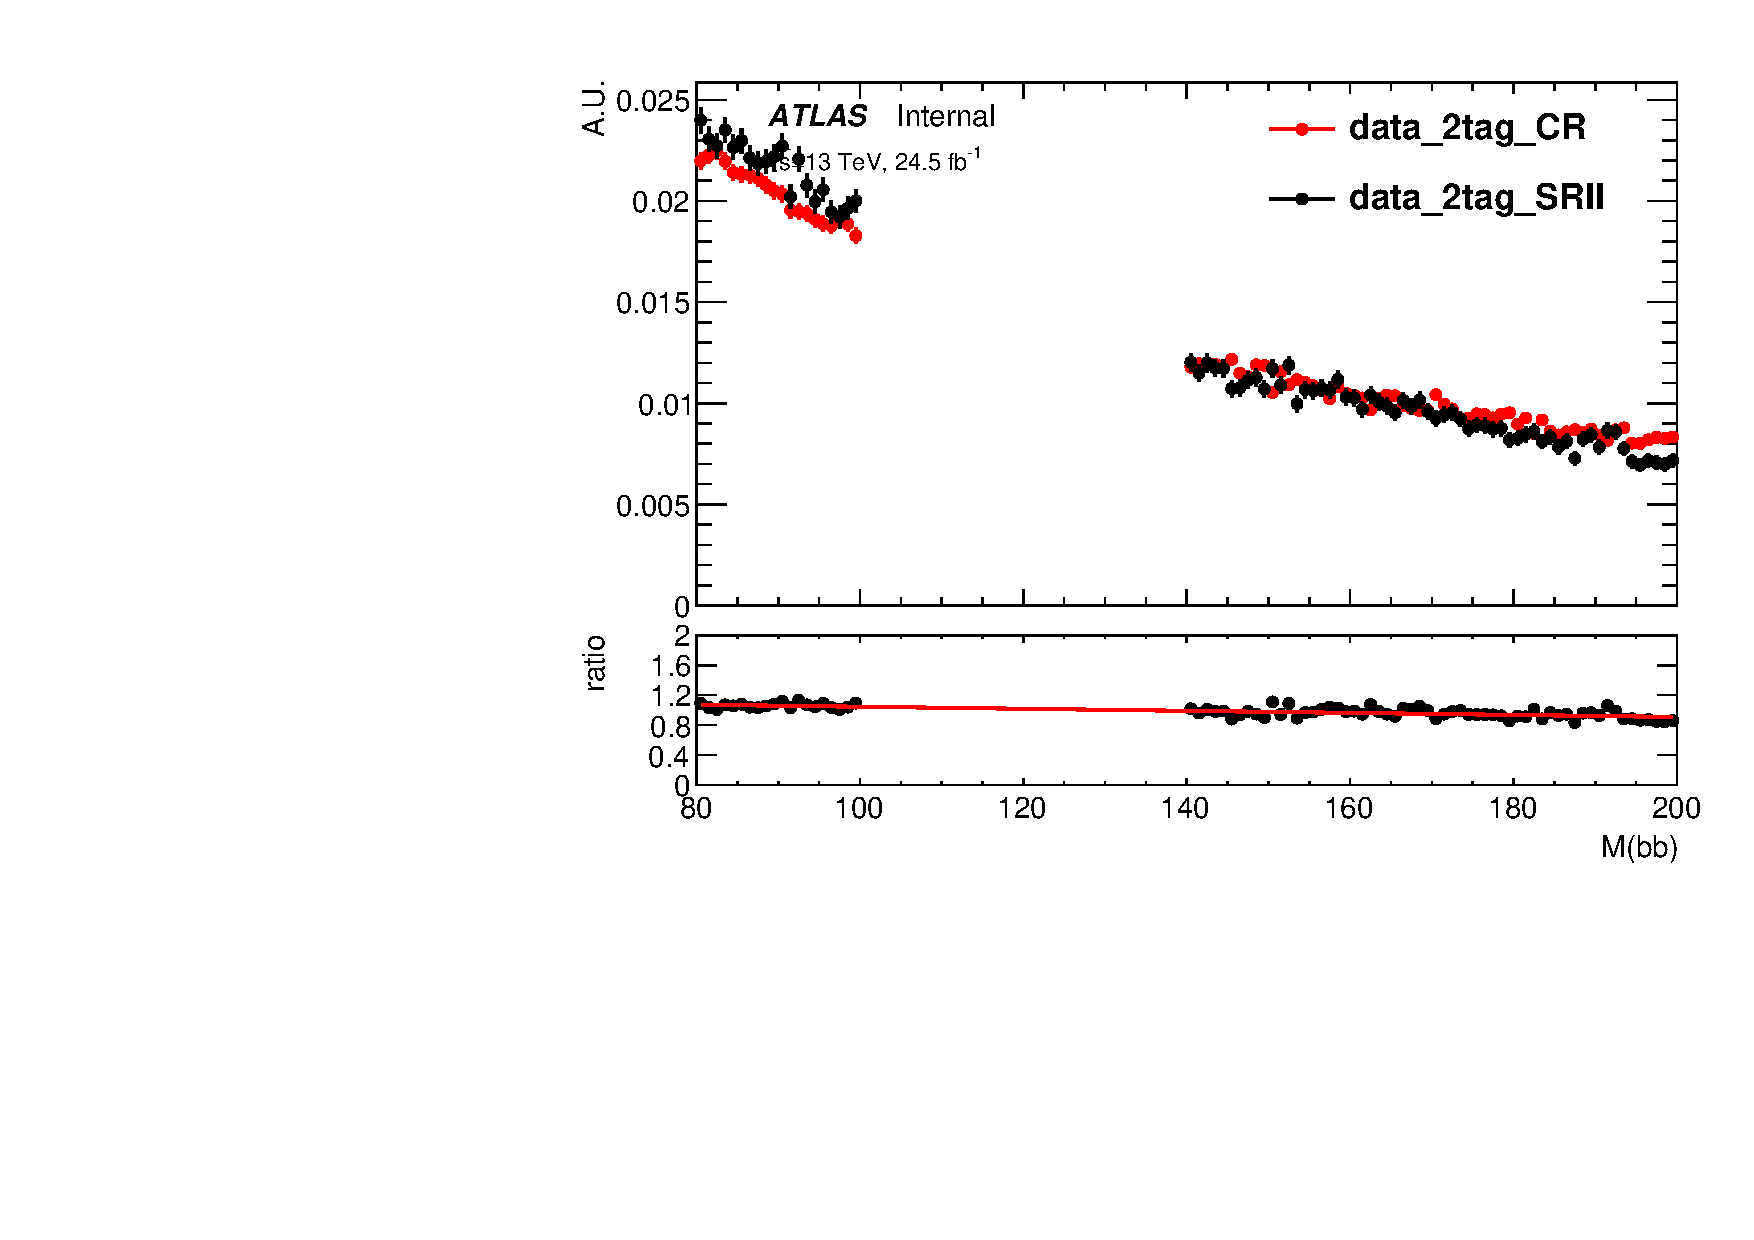
\includegraphics[width=0.45\textwidth]{figures/Mbb_CR_SRII_4cen.pdf}\\
 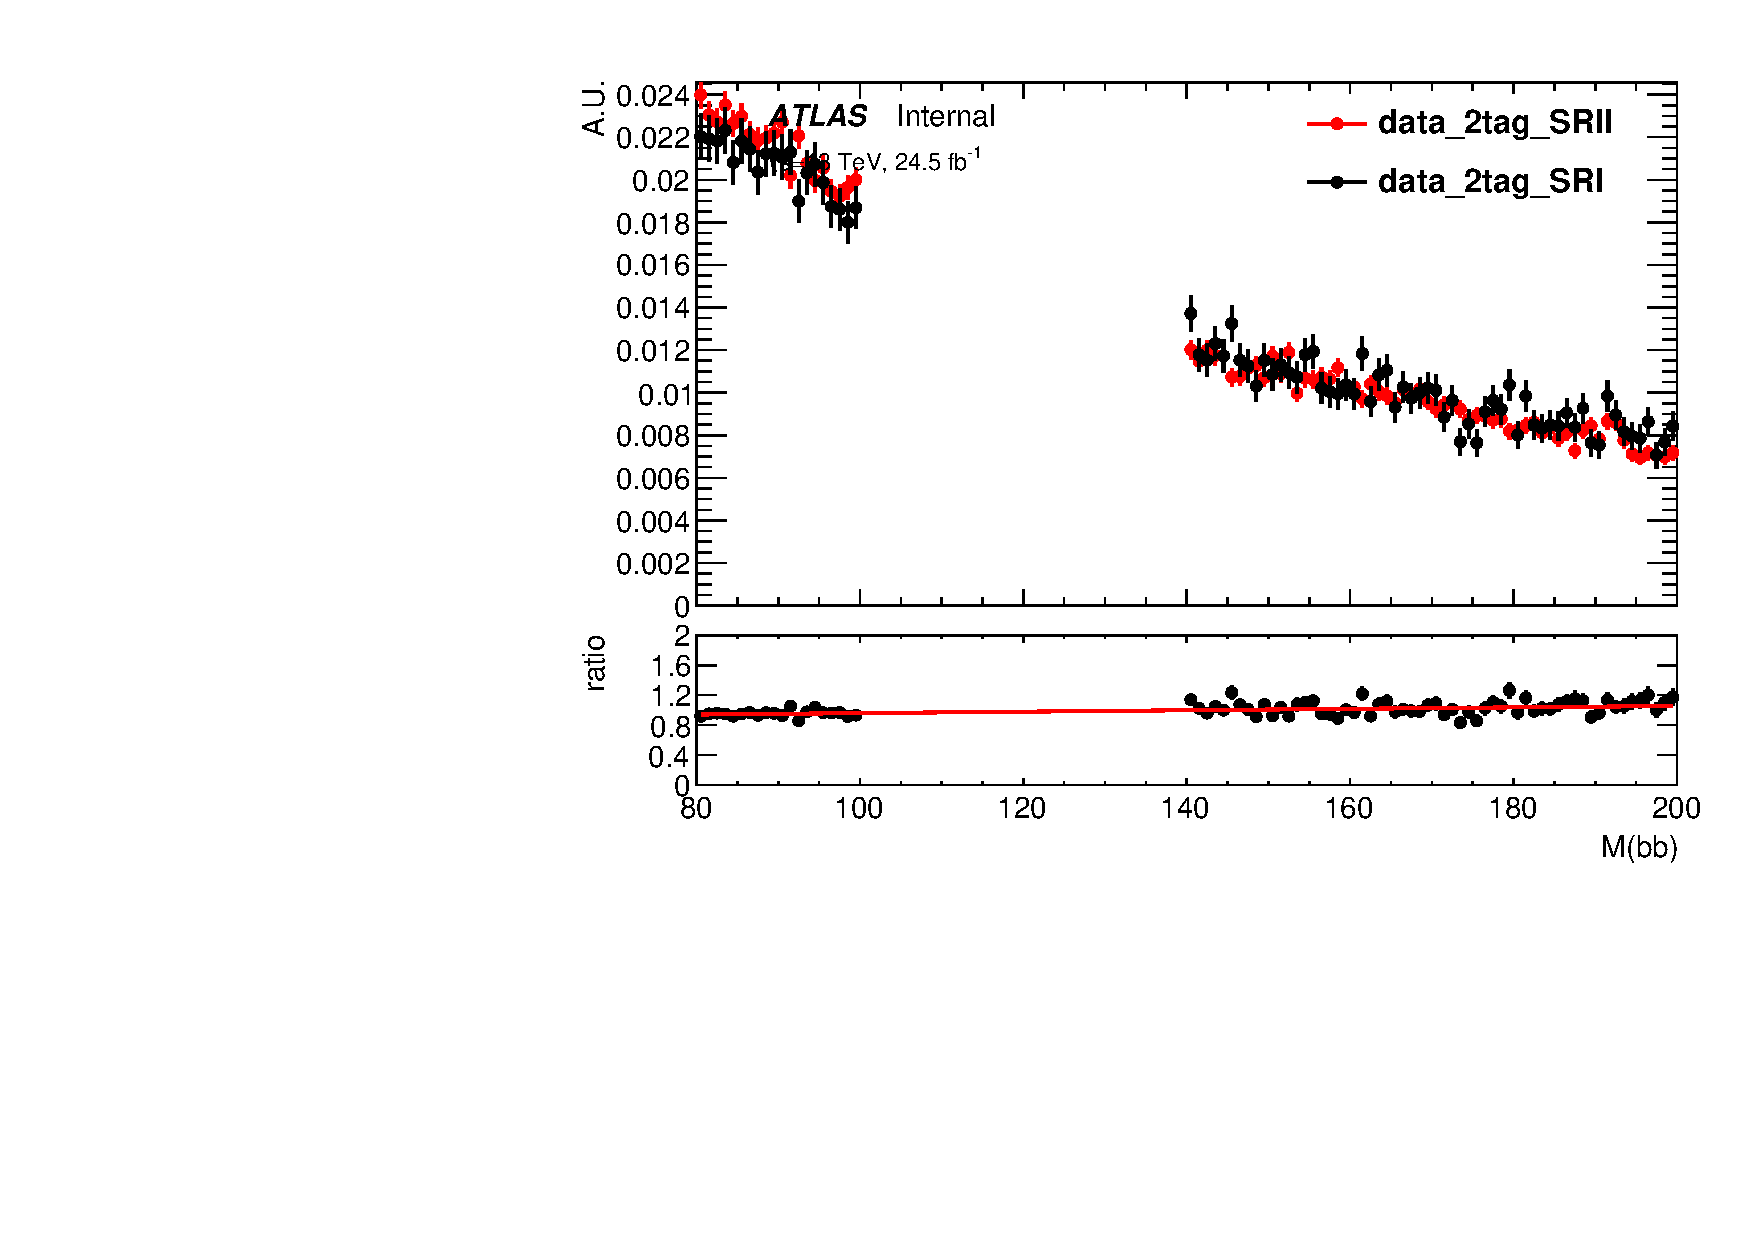
\includegraphics[width=0.45\textwidth]{figures/Mbb_SRI_SRII_4cen.pdf}\\
\caption{\Mbb~shape comparison between CR and both SR for the \fourcentral channel.  The bottom panel in each plot shows the ratio of the two plotted distributions.  The $\chi^2$/ndof of the linear fits are reported in Table~\ref{tab:mbb_lin_4cen-old}.}
  \label{fig:mbb_2tag_4cen-old}
\end{figure}


\begin{table}[htbp]
\centering
\caption{$\chi^2$ of linear fit to signal and control region ratios for the \twocentral channel.}
\label{tab:mbb_lin_2cen-old}
\begin{tabular}{|l|l|l|l|}
\hline
Region                   & SR I Vs. SR II & SR I Vs. SR III & SR II Vs. SR III \\ \hline
Linear Fit $\chi^2$ /nodf & 81.2 / 78   & 83.4 / 78    & 93.0 / 78      \\ \hline
Linear Fit $Prob(\chi^2)$ & 0.38         & 0.32           & 0.12              \\ \hline
Region                   & SR I Vs. CR & SR II Vs. CR & SR III Vs. CR \\ \hline
Linear Fit $\chi^2$ /nodf & 83.5 / 78   & 87.2 / 78    & 71.2 / 78      \\ \hline
Linear Fit $Prob(\chi^2)$ & 0.31         & 0.22           & 0.69              \\ \hline
\end{tabular}
\end{table}


\begin{table}[htbp]
\centering
\caption{$\chi^2$ of linear fit to signal and control region ratios for the \fourcentral channel.}
\label{tab:mbb_lin_4cen-old}
\begin{tabular}{|l|l|l|l|}
\hline
Region                   & SR I Vs. CR & SR II Vs. CR & SR I Vs. SR II \\ \hline
Linear Fit $\chi^2$ /nodf & 67.0 / 78   & 92.5/ 78    & 75.2 / 78      \\ \hline
Linear Fit $Prob(\chi^2)$ & 0.81         & 0.13           & 0.58              \\ \hline
\end{tabular}
\end{table}

\paragraph{Function choice}

Several functions are considered and tested. The functions are required to pass two conditions:

\begin{itemize}
\item Compatibility: The function must be statistically 
compatible with the sidebands of the \Mbb{} distribution in the signal regions,
where the Higgs mass range $100<\Mbb<140$ GeV is ignored. The compatibility criterion is defined as $P(\chi^2)>0.05$ and $P(F-\rm{test})>0.05$, 
where the $\chi^2$ and $F-\rm{test}$ probabilities are considered, respectively.
The $F-\rm{test}$ is performed with respect to the $n+1$ order function.  Only statistical errors are considered in these fits. 

\item Spurious Signal: No significant spurious signal in the Higgs mass window of the control region should arise.  The spurious signal is defined as the size of the apparent signal strength, $\mu_{\rm sp}$, in the control region.  It could arise if the residual between the fitting function and data is biased, and the bias is compatible with the shape of a resonance. The spurious signal induced in the Higgs mass region is estimated 
for each candidate function using the full \Mbb{} distribution in the control region
fitted with the resonant signal distribution for each signal region.
To calculate the apparent strength appropriately for each region, the signal distribution is scaled by the ratio of the number of events in the control region side-bands to the number of events in the signal region sidebands.%to match the control region statistics.
Only statistical errors are considered in these fits. The chosen function is required 
to yield a statistically insignificant spurious signal.  It must be less than one $\sigma$  deviation from 0.  

The spurious signal test has the limitation that it is subject to the statistical power of the control region, which is not very high for this analysis.  However, it is currently the most well-defined test we have for assessing the potential bias of the fitting function given that we do not have non-resonant background MC events.

\end{itemize}

 
Among the candidates satisfying the conditions above, the function with the smallest
number of degrees of freedom is chosen.
For this study, the \zjets{} component is included in the fit, 
normalized to the SM prediction.

The family of functions considered is that of the Bernstein polynomials listed in Equation~\ref{eq:bernstein}, which were
used successfully in the previous iteration of this analysis.  The product of Bernstein and exponential functions were also tried but did not give any improvements with respect to the Bernstein-only functions.

%\begin{equation}
%\label{eq:bernstein}
%\begin{aligned}
%\textnormal{Berstein O2} &= a_1(1-k)^2 + 2a_2(1-k)k + a_3k^2, \\
%\textnormal{Berstein O3} &= a_1(1-k)^3 + 3a_2(1-k)^2k + 3a_3(1-k)k^2 + a_4k^3, \\
%\textnormal{Berstein O4} &= a_1(1-k)^4 + 4a_2(1-k)^3k + 6a_3(1-k)^2k^2 + 4a_4(1-k)k^3 + a_5k^4,\\
%\textnormal{Berstein O5} &= a_1(1-k)^5 + 5a_2(1-k)^4k + 10a_3(1-k)^3k^2 + 10a_4(1-k)^2k^3 + 5a_5(1-k)k^4 +a_6k^5, \\
%\textnormal{where } k &\equiv \frac{(x-80)}{120}
%\end{aligned}
%\end{equation}


The $\chi^2$ values and probabilities  
and $F-\rm{test}$ probabilities are summarized in Tables~\ref{tab:chi2-old} and ~\ref{tab:f-test-old}. The $\chi^2$ test criteria are met for the O(3) Bernstein function in all regions. The $F$-test is passed for the O(3) for all signal regions and samples.  
  
The spurious signal fits are shown in Figures~\ref{fig:Fit_SP_2cen-old} and~\ref{fig:Fit_SP_4cen-old}.   The spurious signal sizes and errors scaled by the ratio of the number of events in the signal and control region side-bands are given in Table~\ref{tab:spurious-old}.  It can be seen that, for the \twocentral channel, an O(3) Bernstein gives a statistically insignificant spurious signal in all signal regions.   

We choose the O(3) Bernstein as our default fit function for both the \twocentral channel and the \fourcentral channel as it satisfies the function conditions in all signal regions.

\begin{table}[htbp]
\centering
\caption{Background Only Fit $\chi^2$ and Prob($\chi^2$)}
\label{tab:chi2-old}
\begin{tabular}{|l|l|l|l|l|l|l|}
\hline
Channel                     & \multicolumn{3}{c|}{\twocentral} & \multicolumn{2}{c|}{\fourcentral} \\ \hline
Region                      & SR I     & SR II     & SR III    & SR I     & SR II     \\ \hline
Bernstein O2 $\chi^2$/ndof  & 1.19     & 1.15      & 1.15      & 1.16     & 1.29      \\ \hline
Bernstein O2 prob($\chi^2$) & 0.22     & 0.21      & 0.17      & 0.19     & 0.10      \\ \hline
Bernstein O3 $\chi^2$/ndof  & 1.13     & 1.13      & 1.11      & 0.87     & 1.13      \\ \hline
Bernstein O3 prob($\chi^2$) & 0.20     & 0.21      & 0.25      & 0.75     & 0.27      \\ \hline
Bernstein O4 $\chi^2$/ndof  & 1.04     & 1.13      & 1.07      & 0.88     & 1.02      \\ \hline
Bernstein O4 prob($\chi^2$) & 0.39     & 0.21      & 0.32      & 0.72     & 0.43      \\ \hline
Bernstein O5 $\chi^2$/ndof  & 1.03     & 1.14      & 1.06      & 0.89     & 0.95      \\ \hline
Bernstein O5 prob($\chi^2$) & 0.40     & 0.18      & 0.33      & 0.70     & 0.56      \\ \hline
\end{tabular}
\end{table}

\begin{table}[]
\centering
\caption{Background Only Fit F-test}
\label{tab:f-test-old}
\begin{tabular}{|l|l|l|l|l|l|l|}
\hline
Channel          & \multicolumn{3}{c|}{\twocentral} & \multicolumn{2}{c|}{\fourcentral} \\ \hline
Region           & SR I     & SR II     & SR III    & SR I     & SR II   \\ \hline
Bernstein O2/ O3 & 0.52     & 0.52      & 0.43      & 0.34     & 0.14    \\ \hline
Bernstein O3/ O4 & 0.35     & 0.51      & 0.44      & 0.38     & 0.52    \\ \hline
Bernstein O4/ O5 & 0.49     & 0.52      & 0.49      & 0.41     & 0.51    \\ \hline
\end{tabular}
\end{table}


\begin{table}[htbp]
\centering
\caption{Spurious signal size normalized by the ratio of the number of events in the signal  to control region sidebands.}
\label{tab:spurious-old}
\begin{tabular}{|l|l|l|l|l|l|l|}
\hline
 & \multicolumn{5}{c|}{$\mu_{\rm sp}(\sigma_{\mu})$}\\ \hline
Channel       & \multicolumn{3}{c|}{\twocentral}       & \multicolumn{2}{c|}{\fourcentral}       \\ \hline
Region        & SR I        & SR II      & SR III      & SR I        & SR II        \\ \hline
Bernstein  O2 & -1.67(0.64) & -3.86(1.34) & -7.01(2.25) & -3.84(1.49) & -11.76(3.10) \\ \hline
Bernstein  O3 & -0.07(0.81) & -0.61(1.77) & -1.64(3.21) & 0.08(1.24) & 0.31(4.21) \\ \hline
Bernstein  O4 & -0.11(0.79) & -0.68(1.76) & -1.85(3.20) & 0.11(1.25) & 0.37(4.17) \\ \hline
Bernstein  O5 & 0.78(1.08) & 1.44(2.52) & 1.95(5.14)  & 1.79(1.75) & 7.53(6.59) \\ \hline
\end{tabular}
\end{table}


\begin{figure}[htbp]
  \centering
 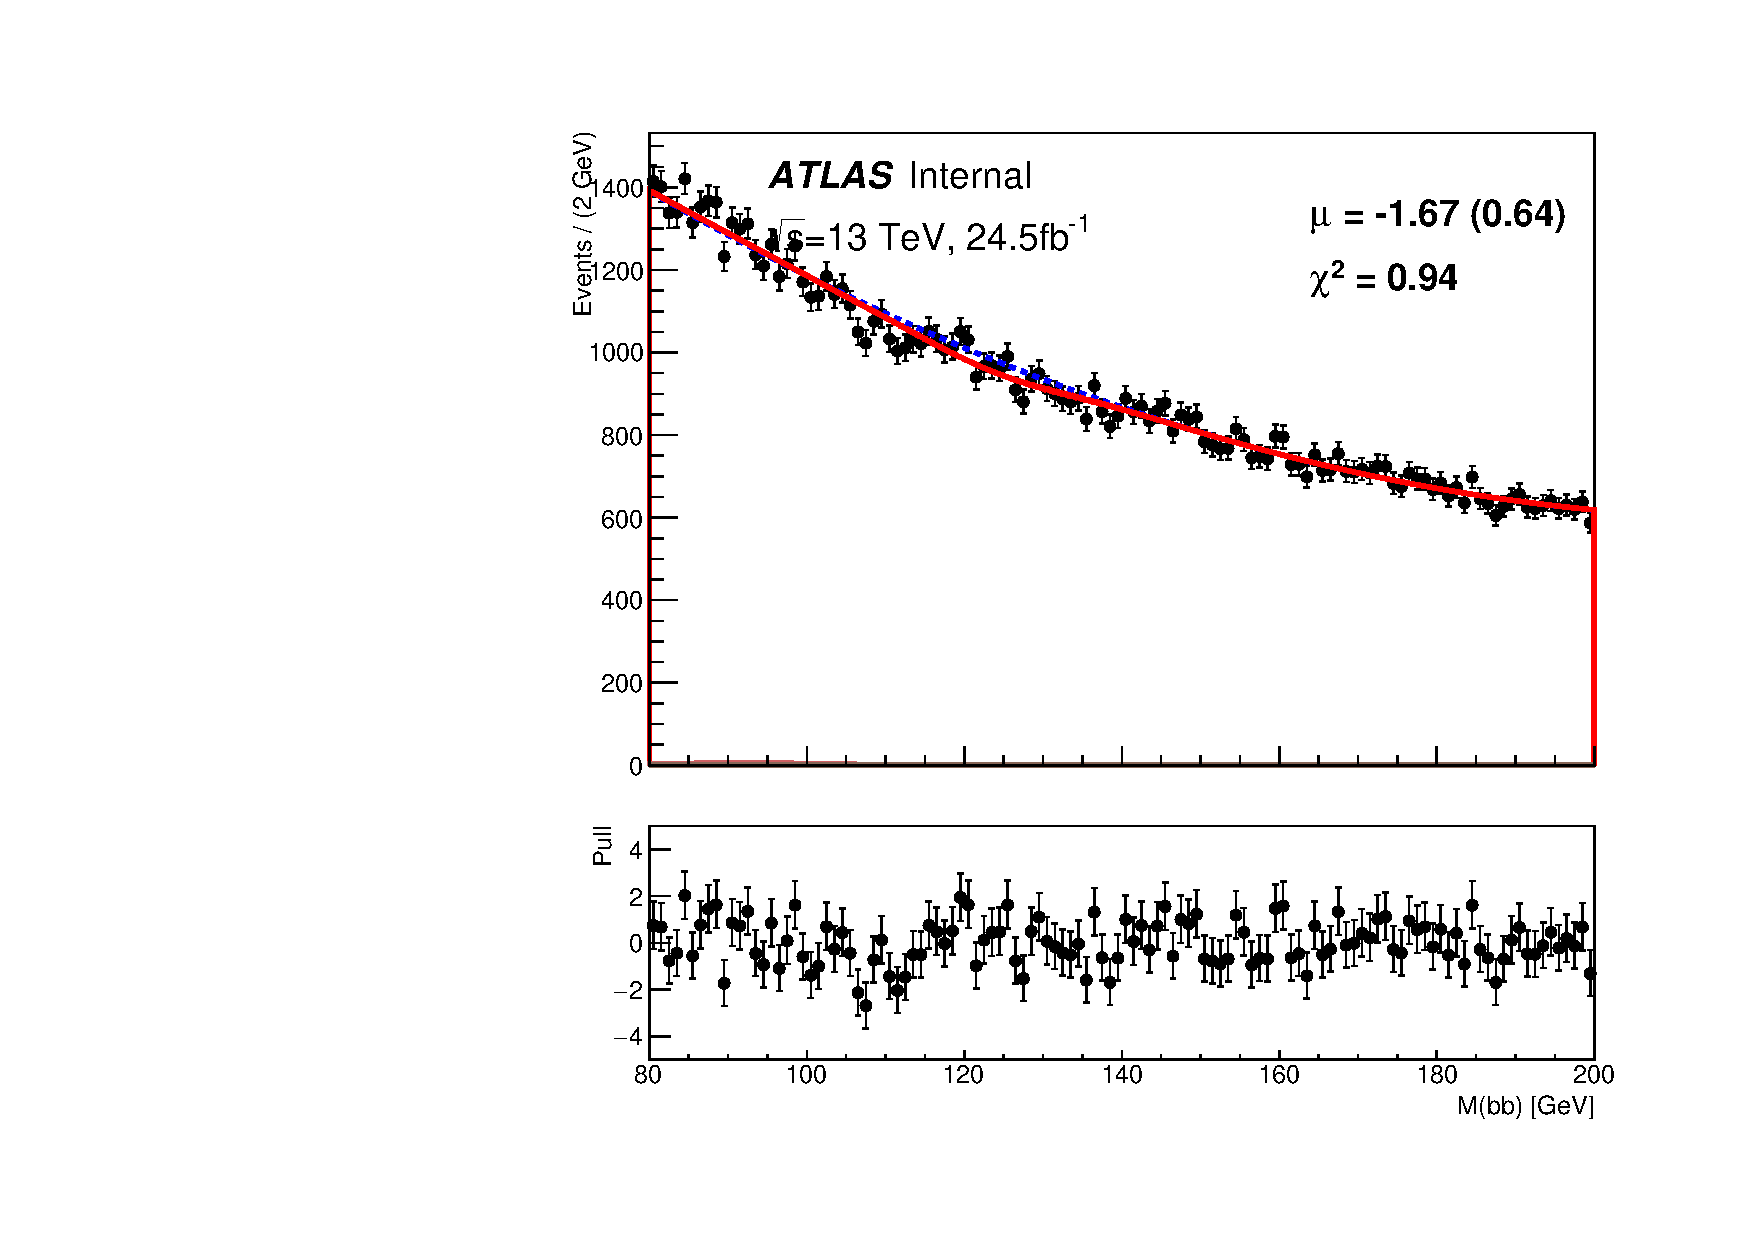
\includegraphics[width=0.24\textwidth]{figures/Fit2cen_SP/spurious_O2_testVBF_ICHEP_2cen_SRI_CTRL.pdf}
 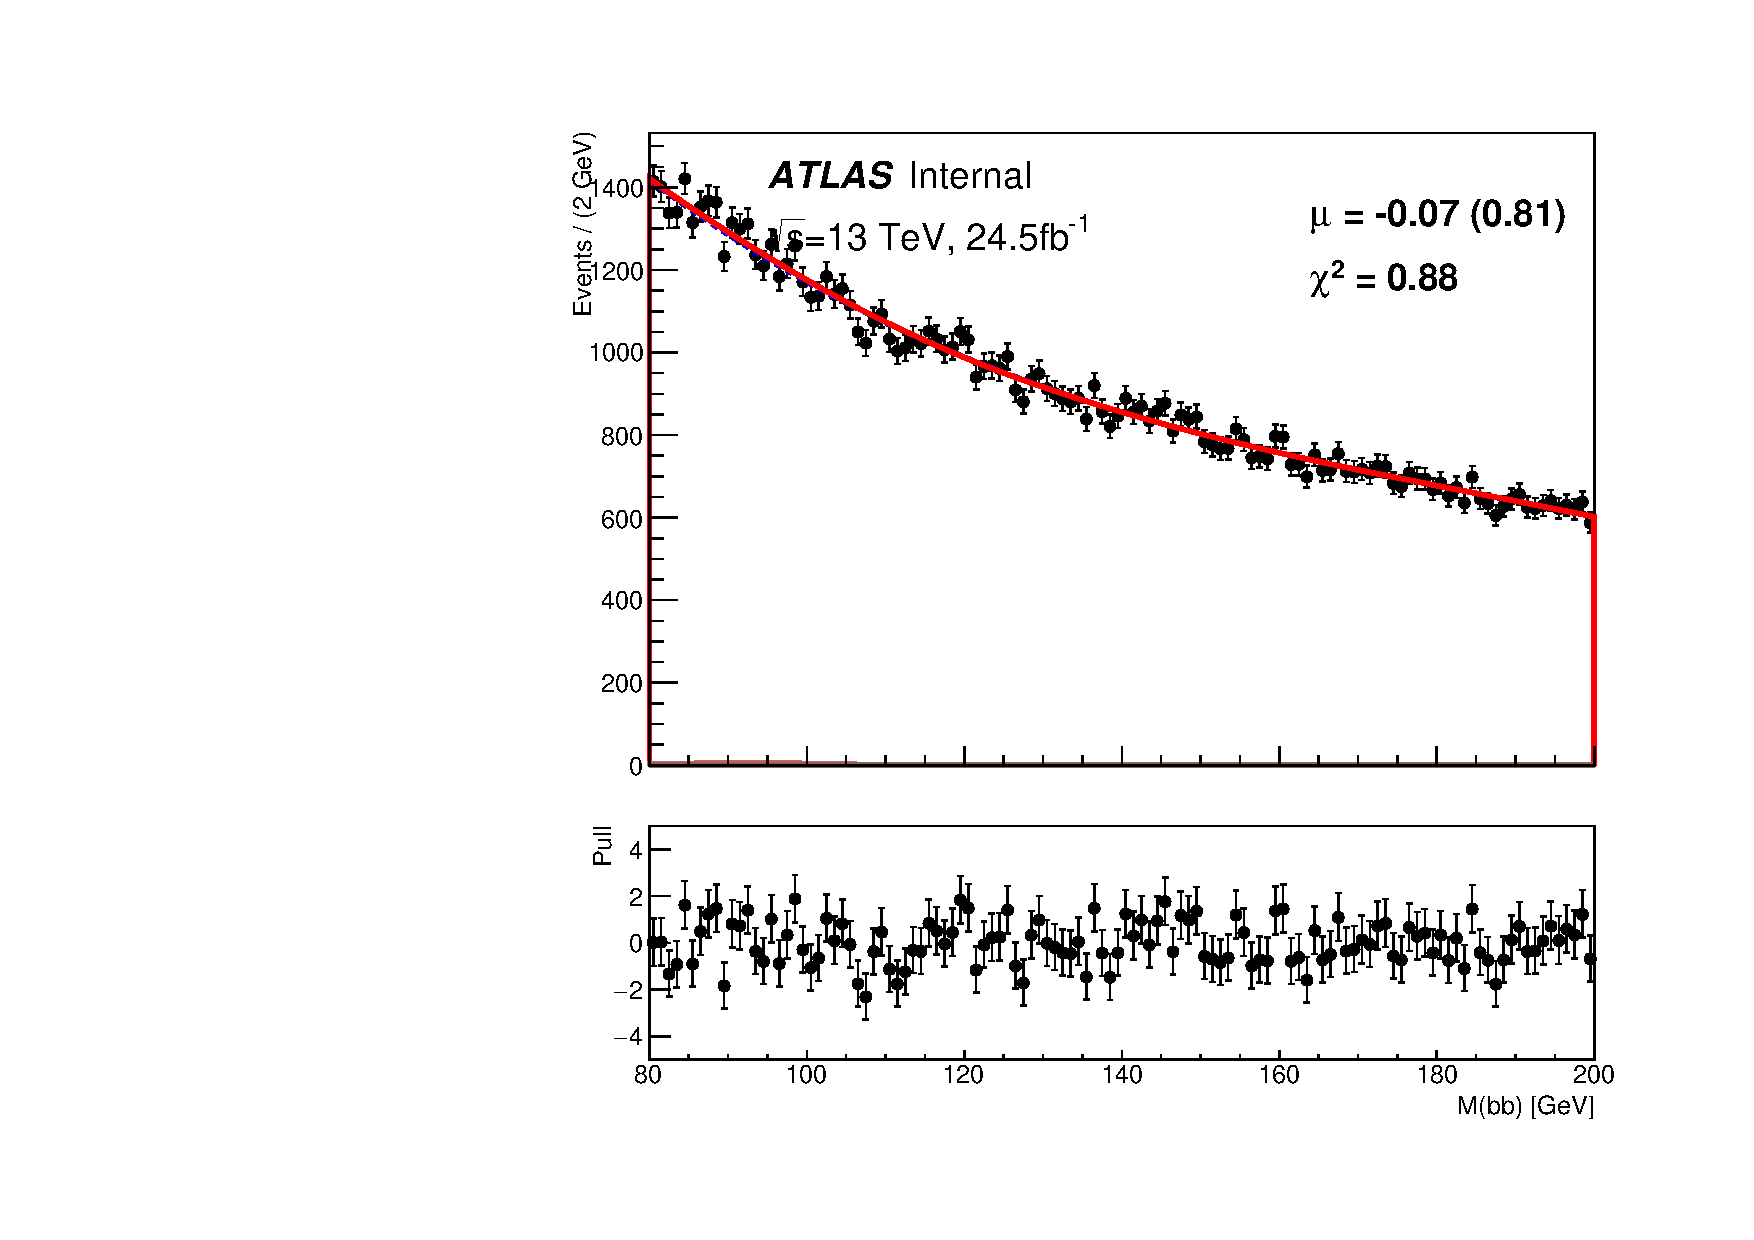
\includegraphics[width=0.24\textwidth]{figures/Fit2cen_SP/spurious_O3_testVBF_ICHEP_2cen_SRI_CTRL.pdf}
 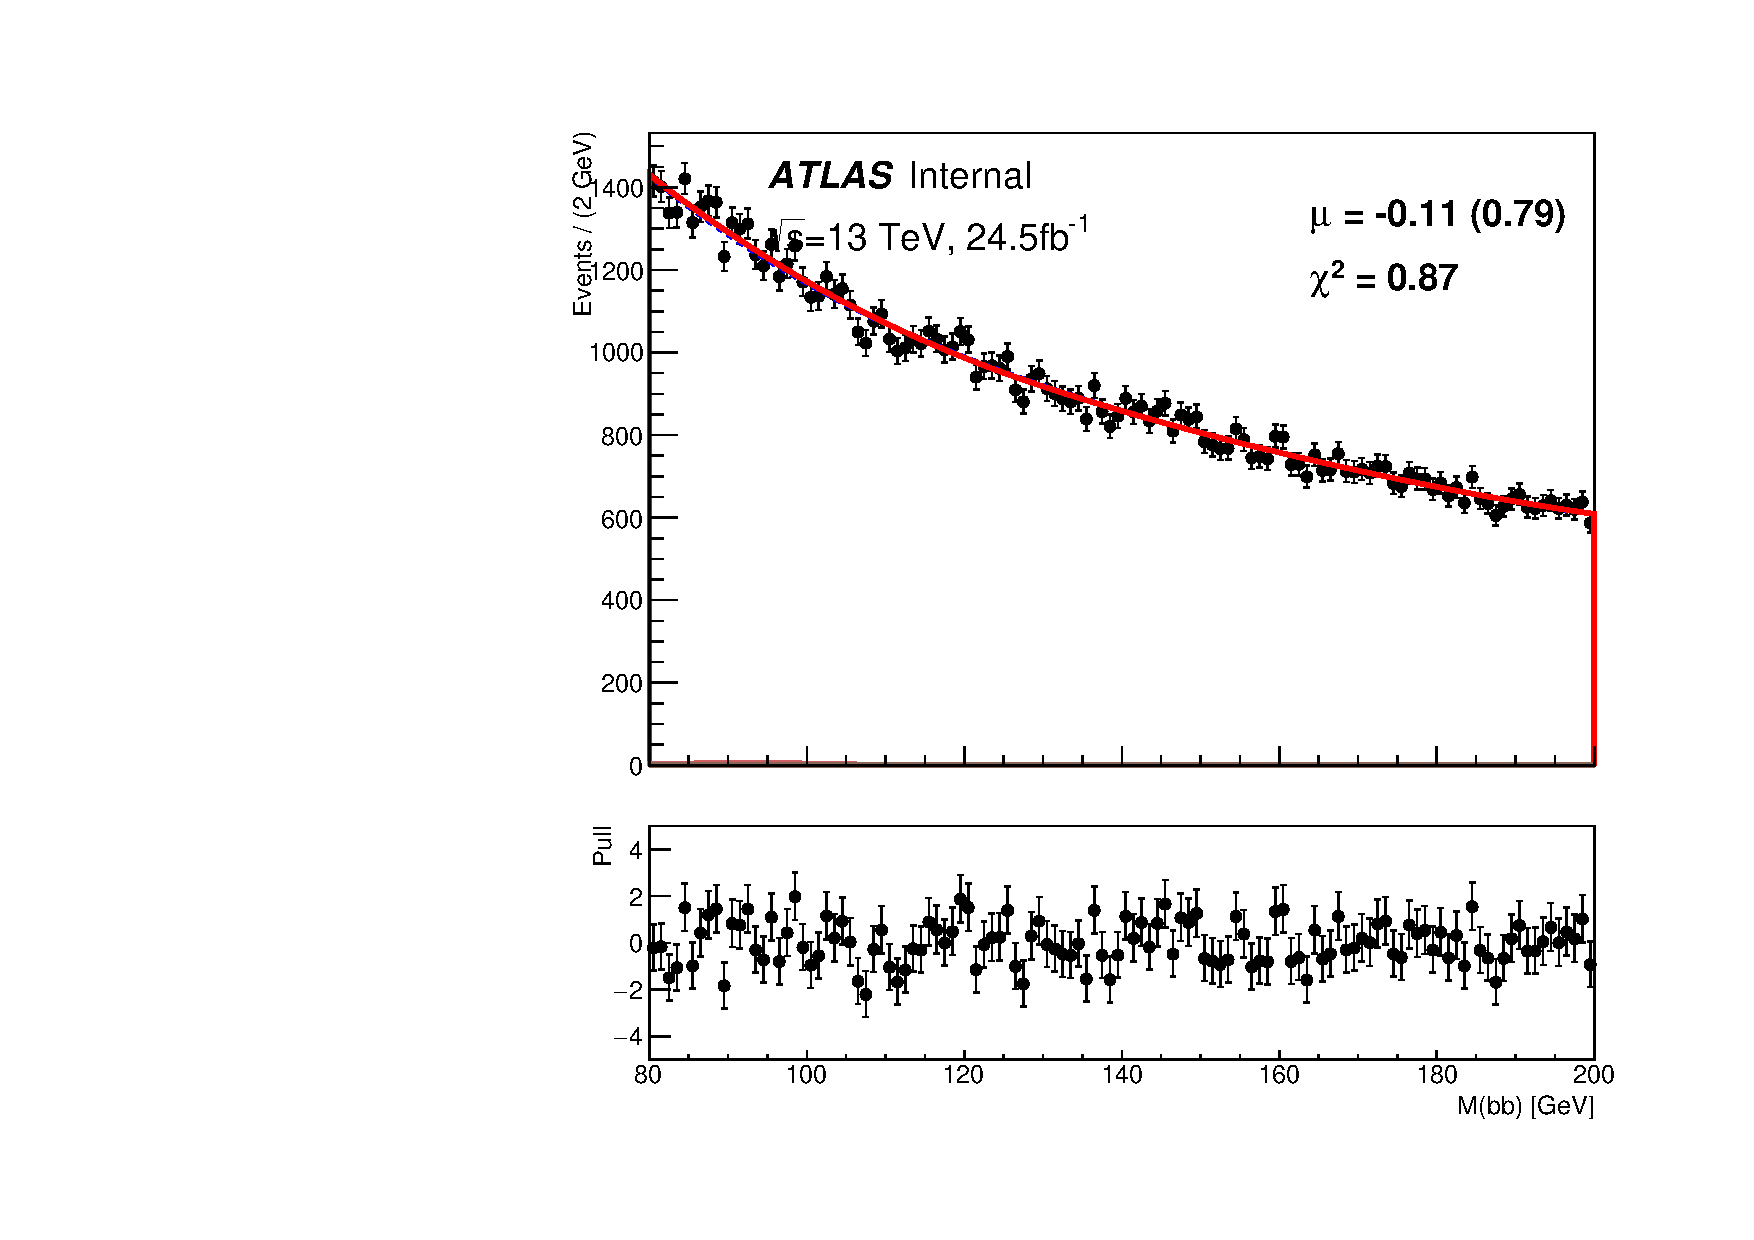
\includegraphics[width=0.24\textwidth]{figures/Fit2cen_SP/spurious_O4_testVBF_ICHEP_2cen_SRI_CTRL.pdf}
 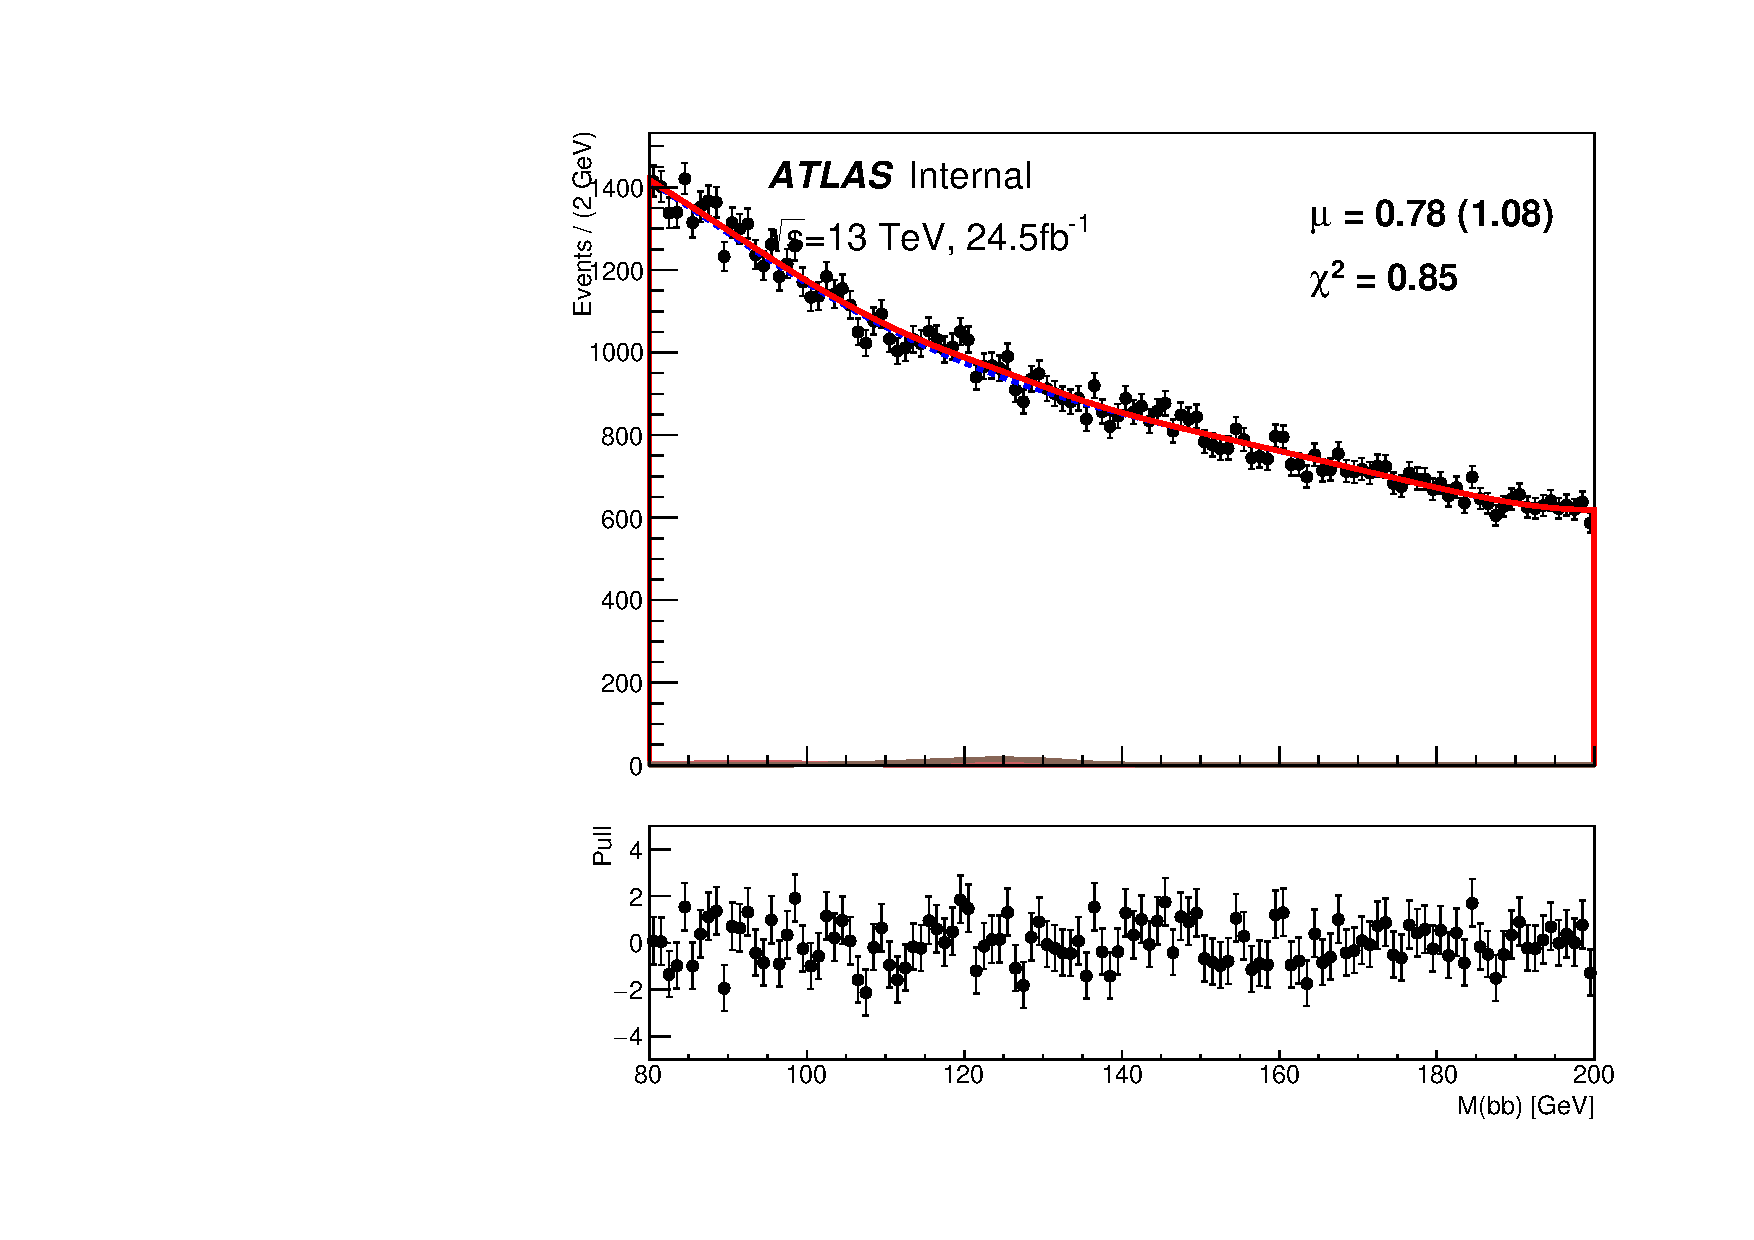
\includegraphics[width=0.24\textwidth]{figures/Fit2cen_SP/spurious_O5_testVBF_ICHEP_2cen_SRI_CTRL.pdf}\\
 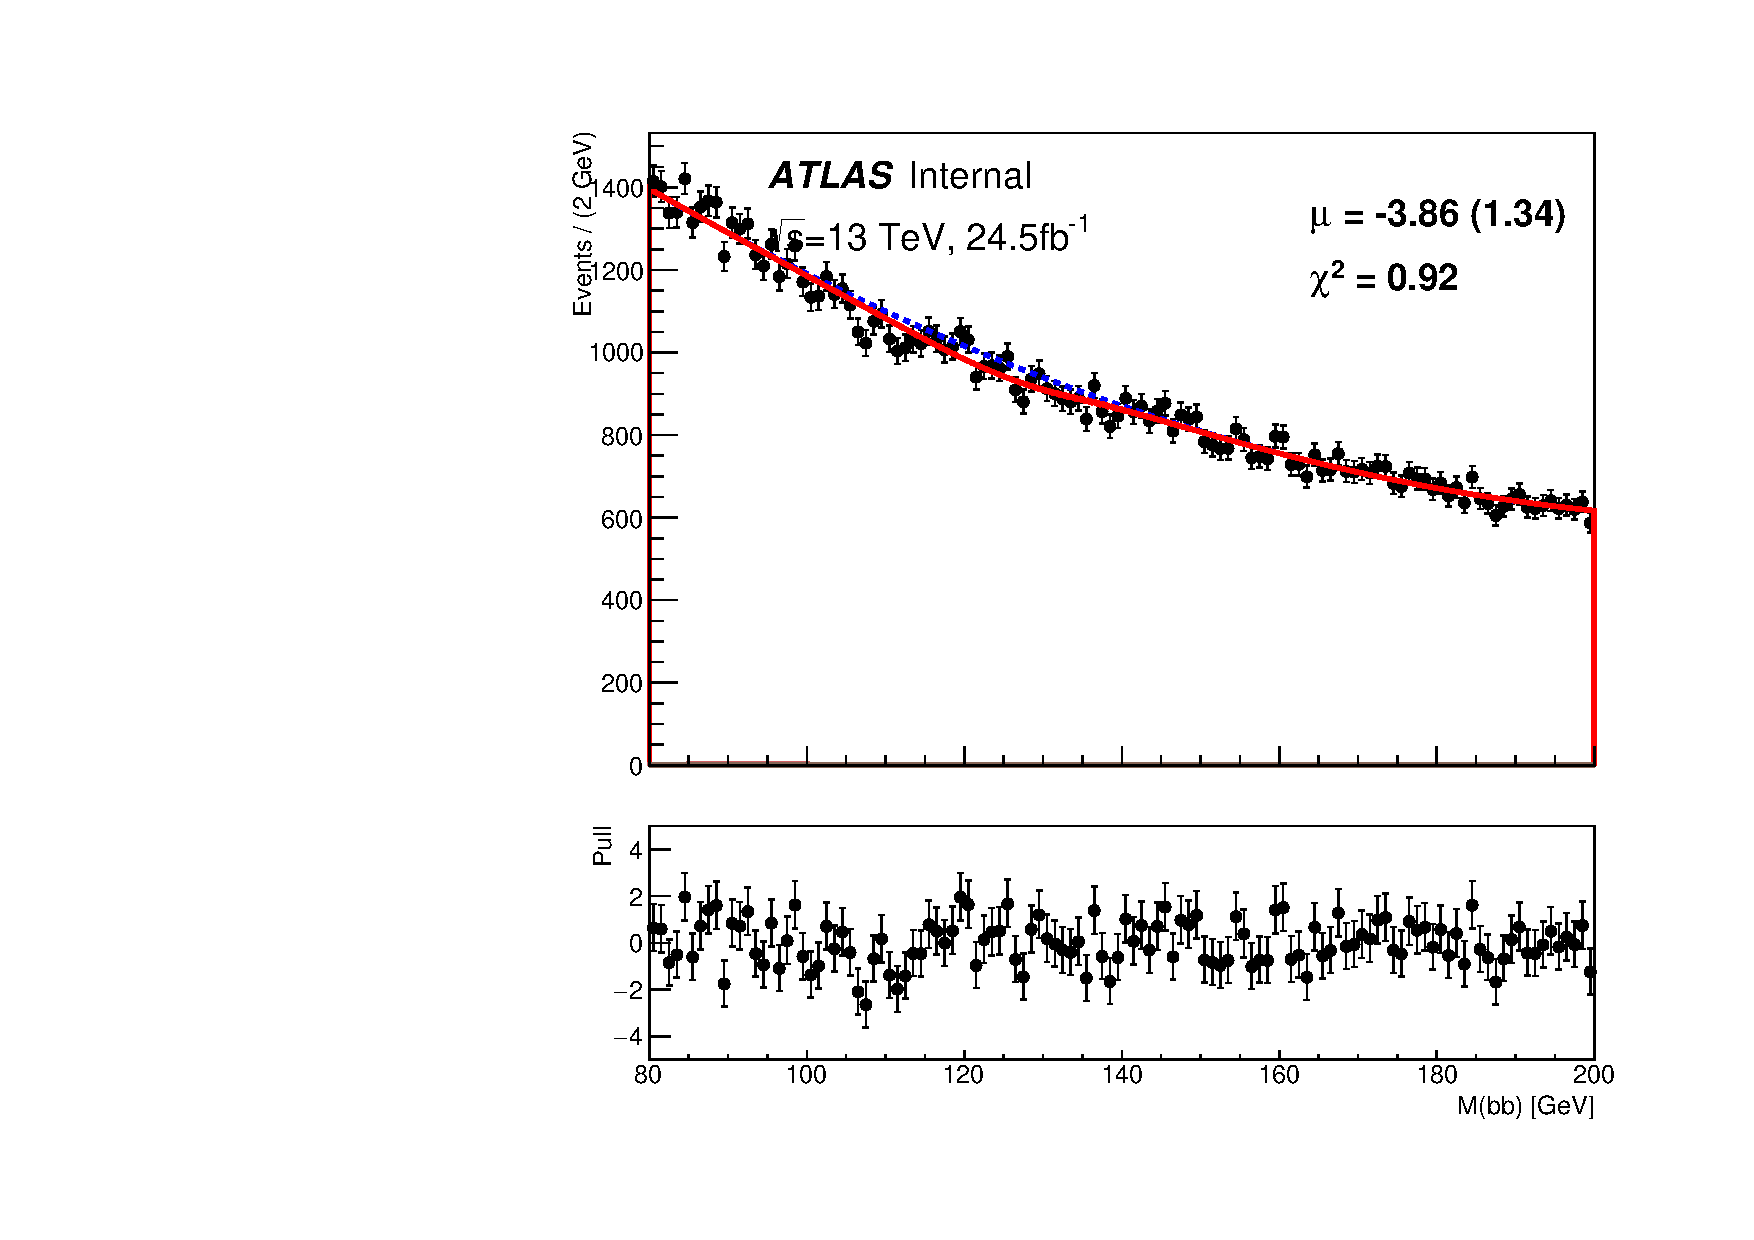
\includegraphics[width=0.24\textwidth]{figures/Fit2cen_SP/spurious_O2_testVBF_ICHEP_2cen_SRII_CTRL.pdf}
 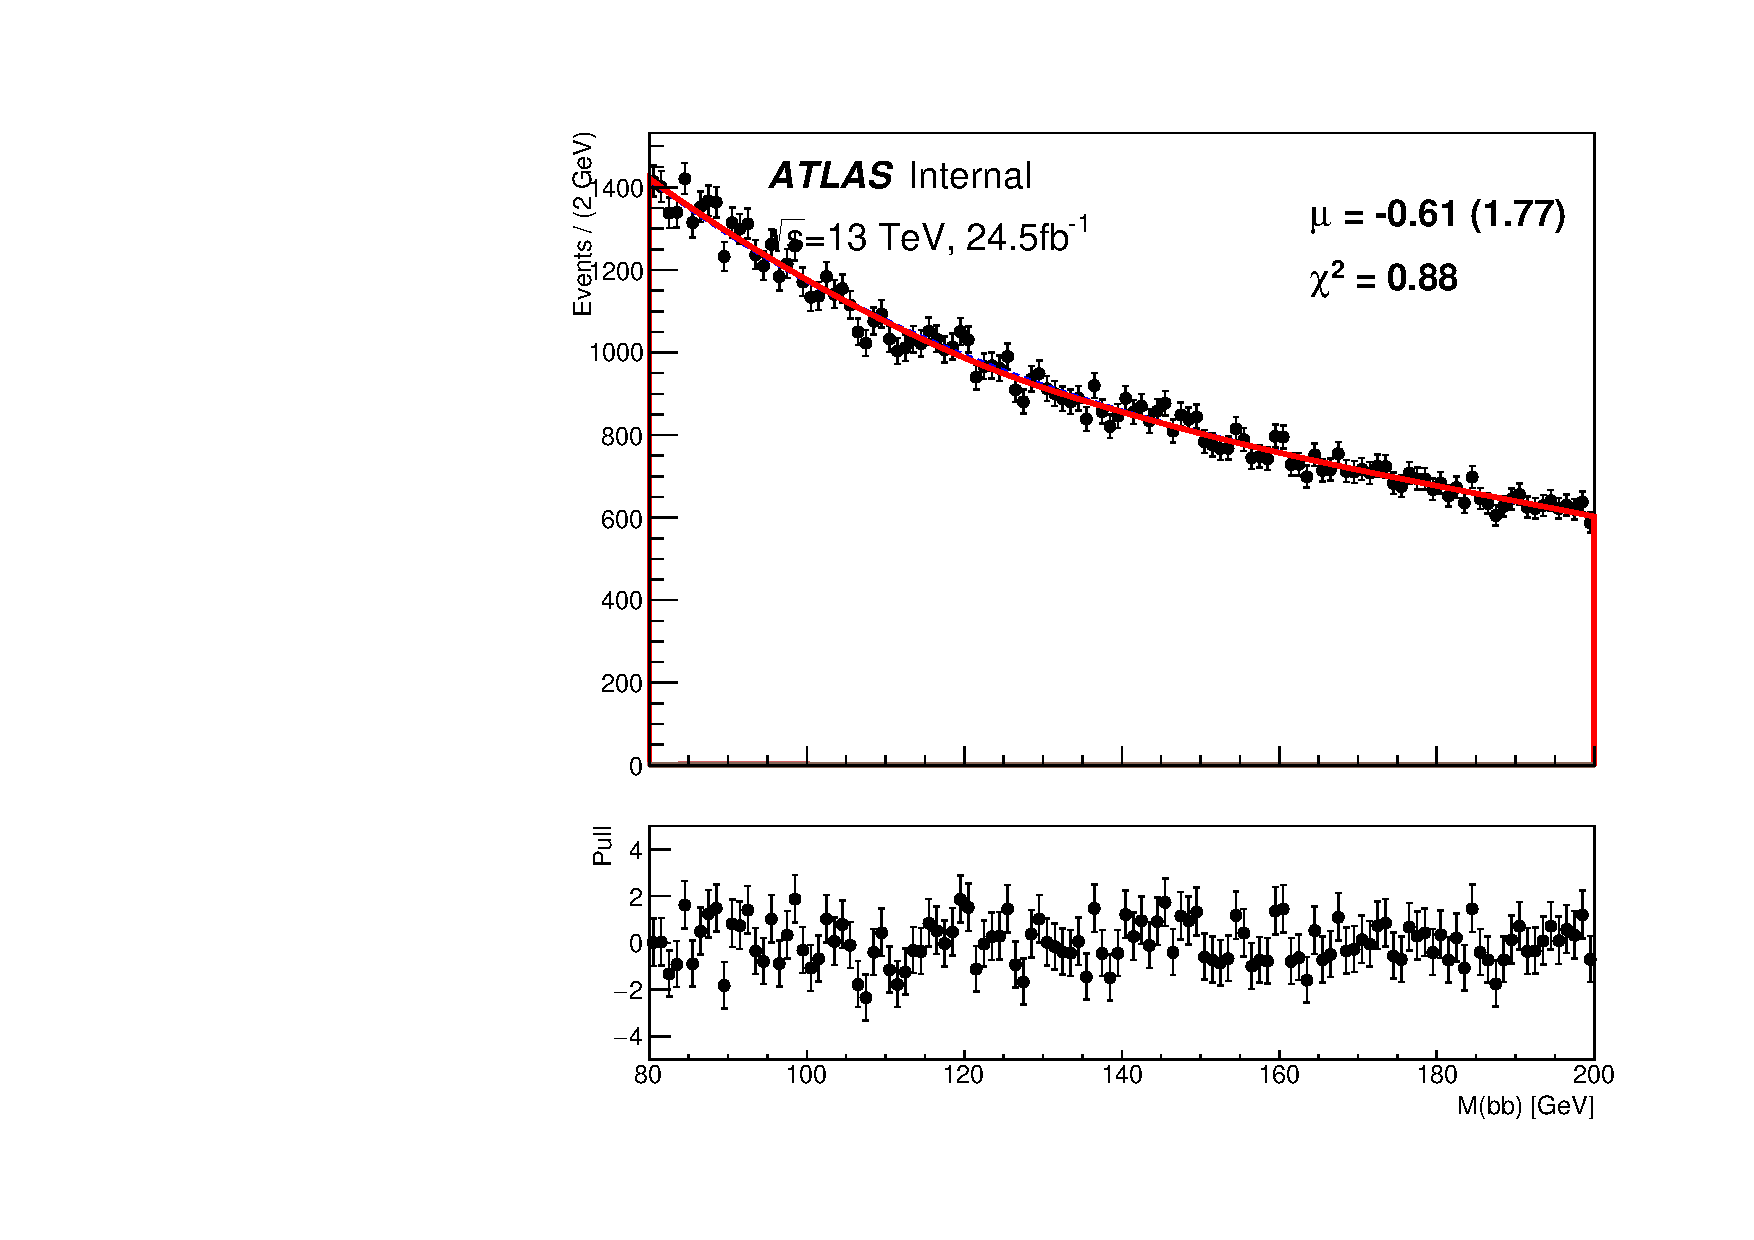
\includegraphics[width=0.24\textwidth]{figures/Fit2cen_SP/spurious_O3_testVBF_ICHEP_2cen_SRII_CTRL.pdf}
 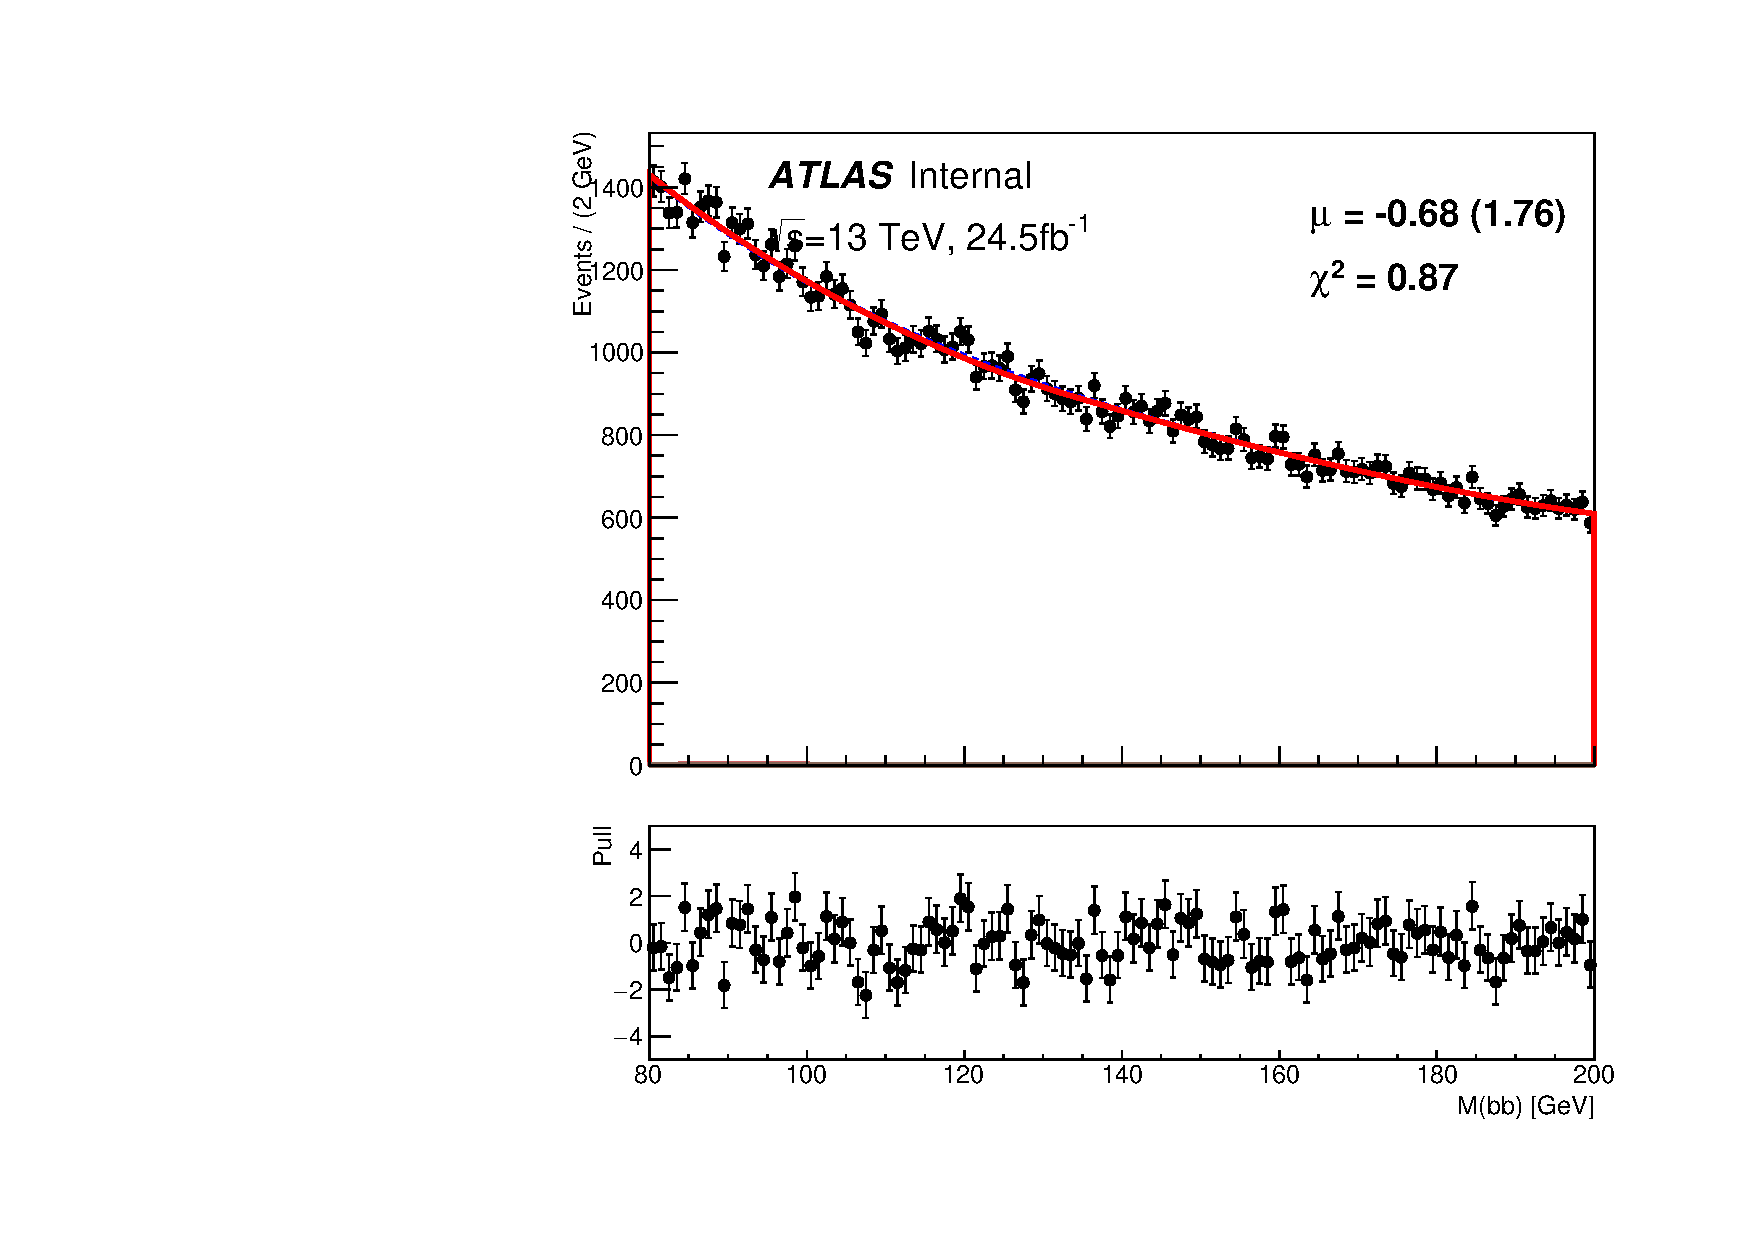
\includegraphics[width=0.24\textwidth]{figures/Fit2cen_SP/spurious_O4_testVBF_ICHEP_2cen_SRII_CTRL.pdf}
 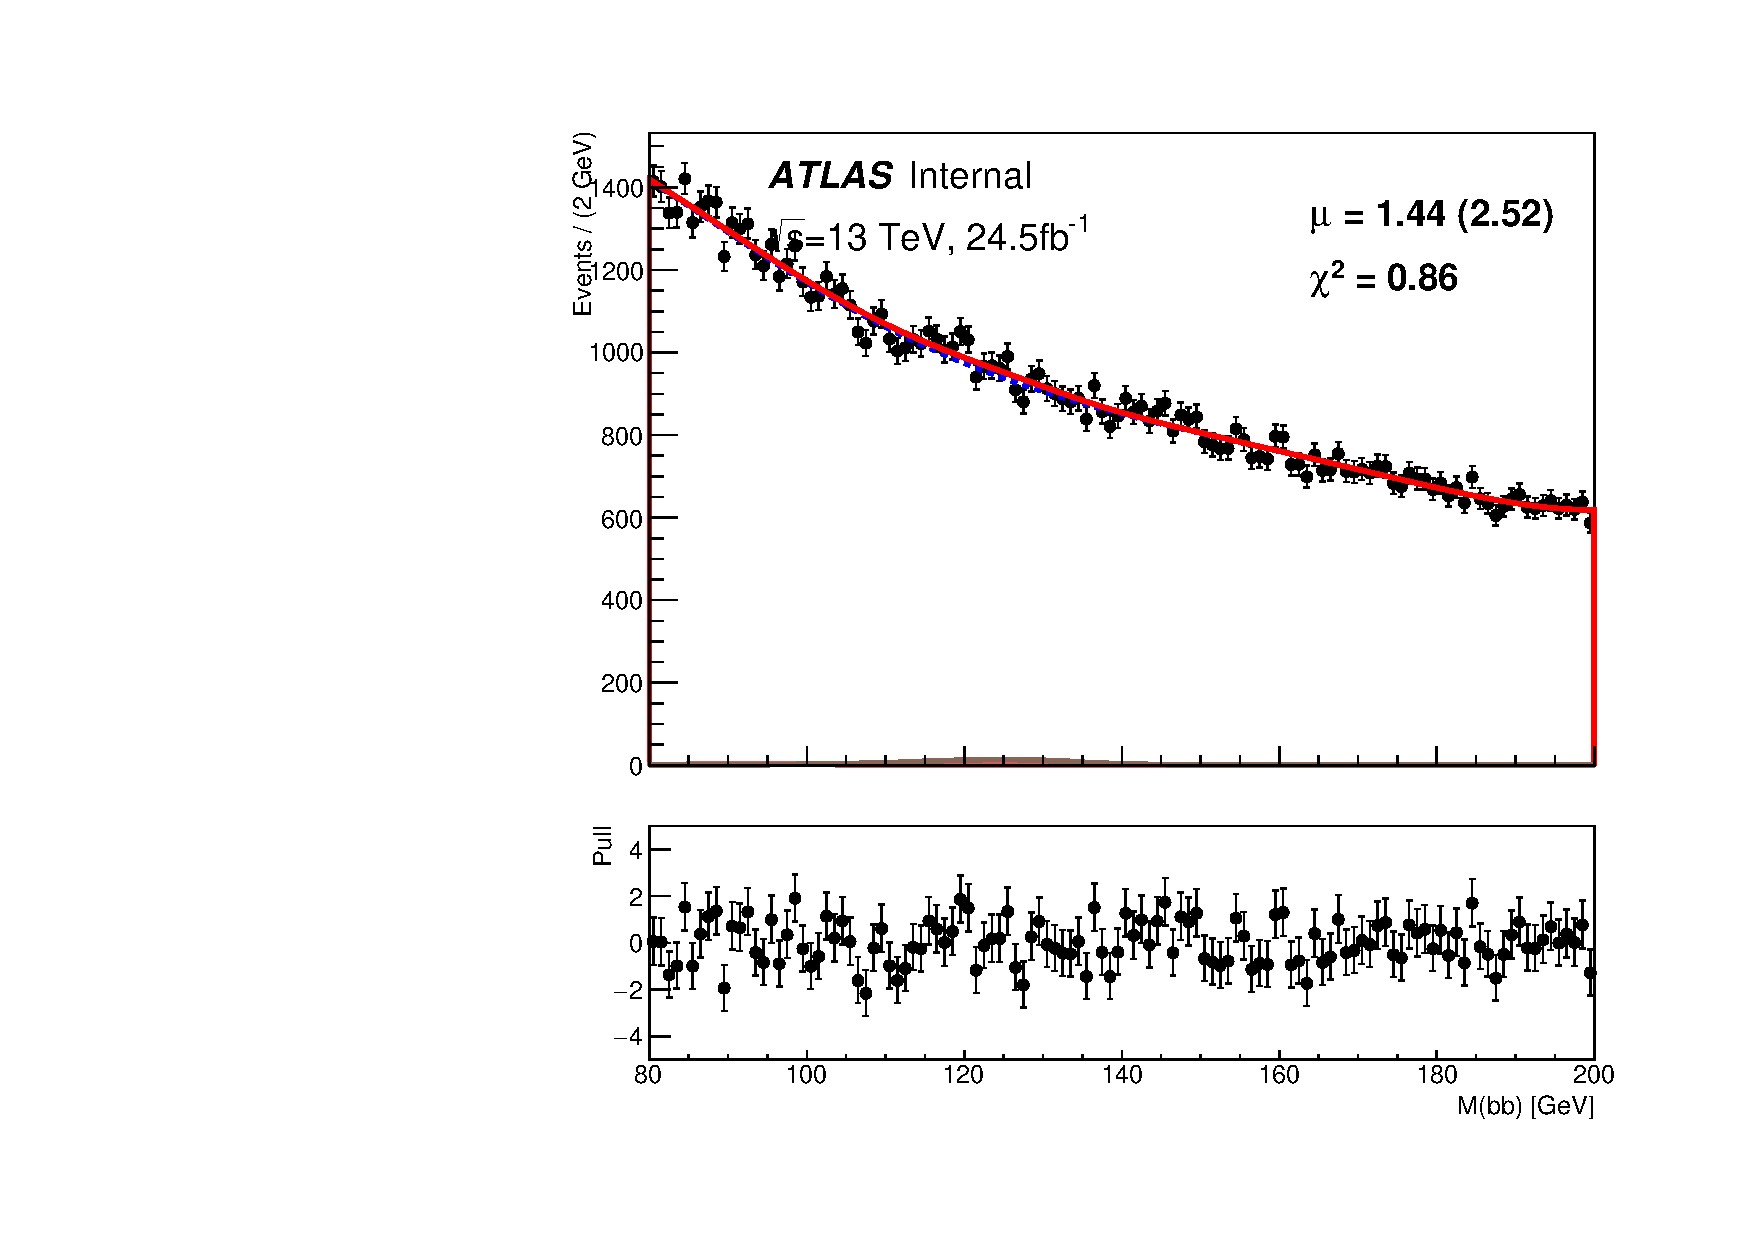
\includegraphics[width=0.24\textwidth]{figures/Fit2cen_SP/spurious_O5_testVBF_ICHEP_2cen_SRII_CTRL.pdf}\\
 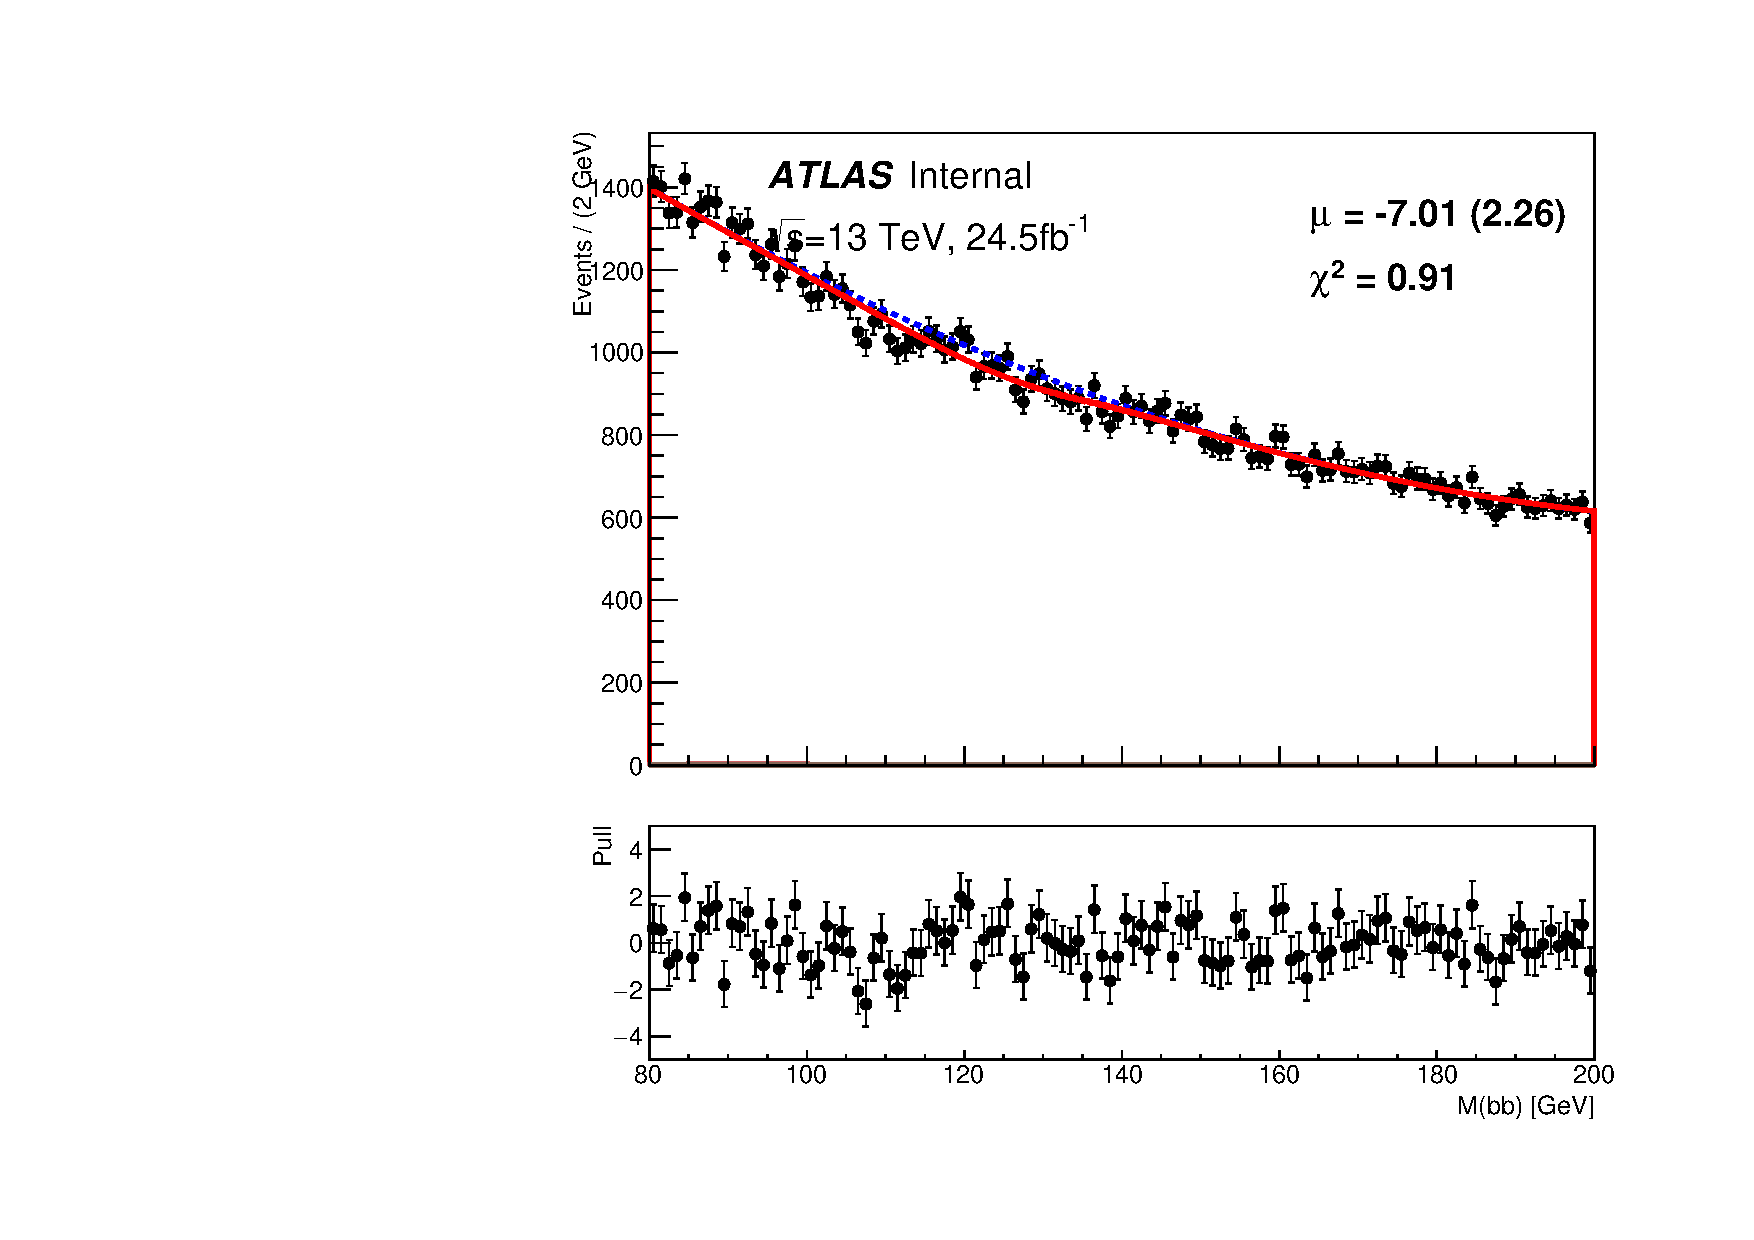
\includegraphics[width=0.24\textwidth]{figures/Fit2cen_SP/spurious_O2_testVBF_ICHEP_2cen_SRIII_CTRL.pdf}
 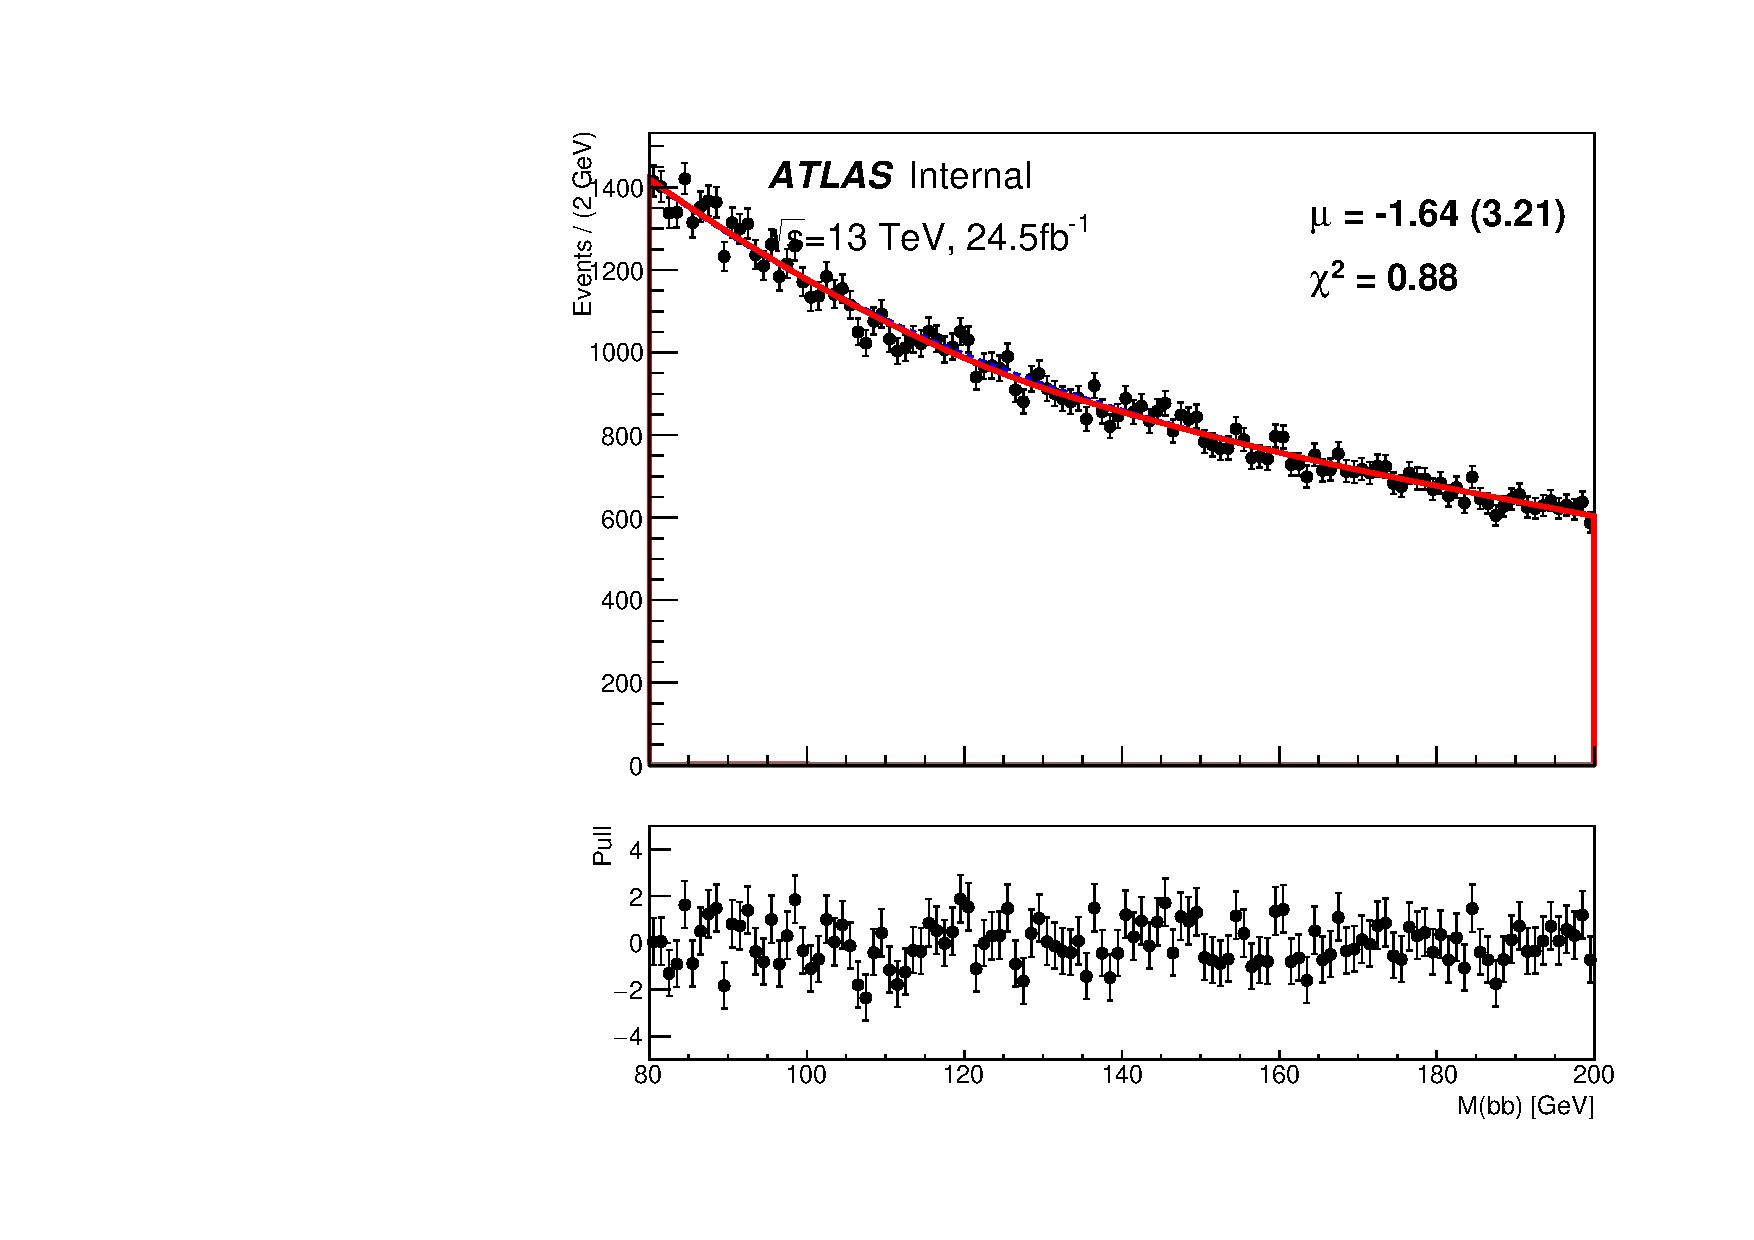
\includegraphics[width=0.24\textwidth]{figures/Fit2cen_SP/spurious_O3_testVBF_ICHEP_2cen_SRIII_CTRL.pdf}
 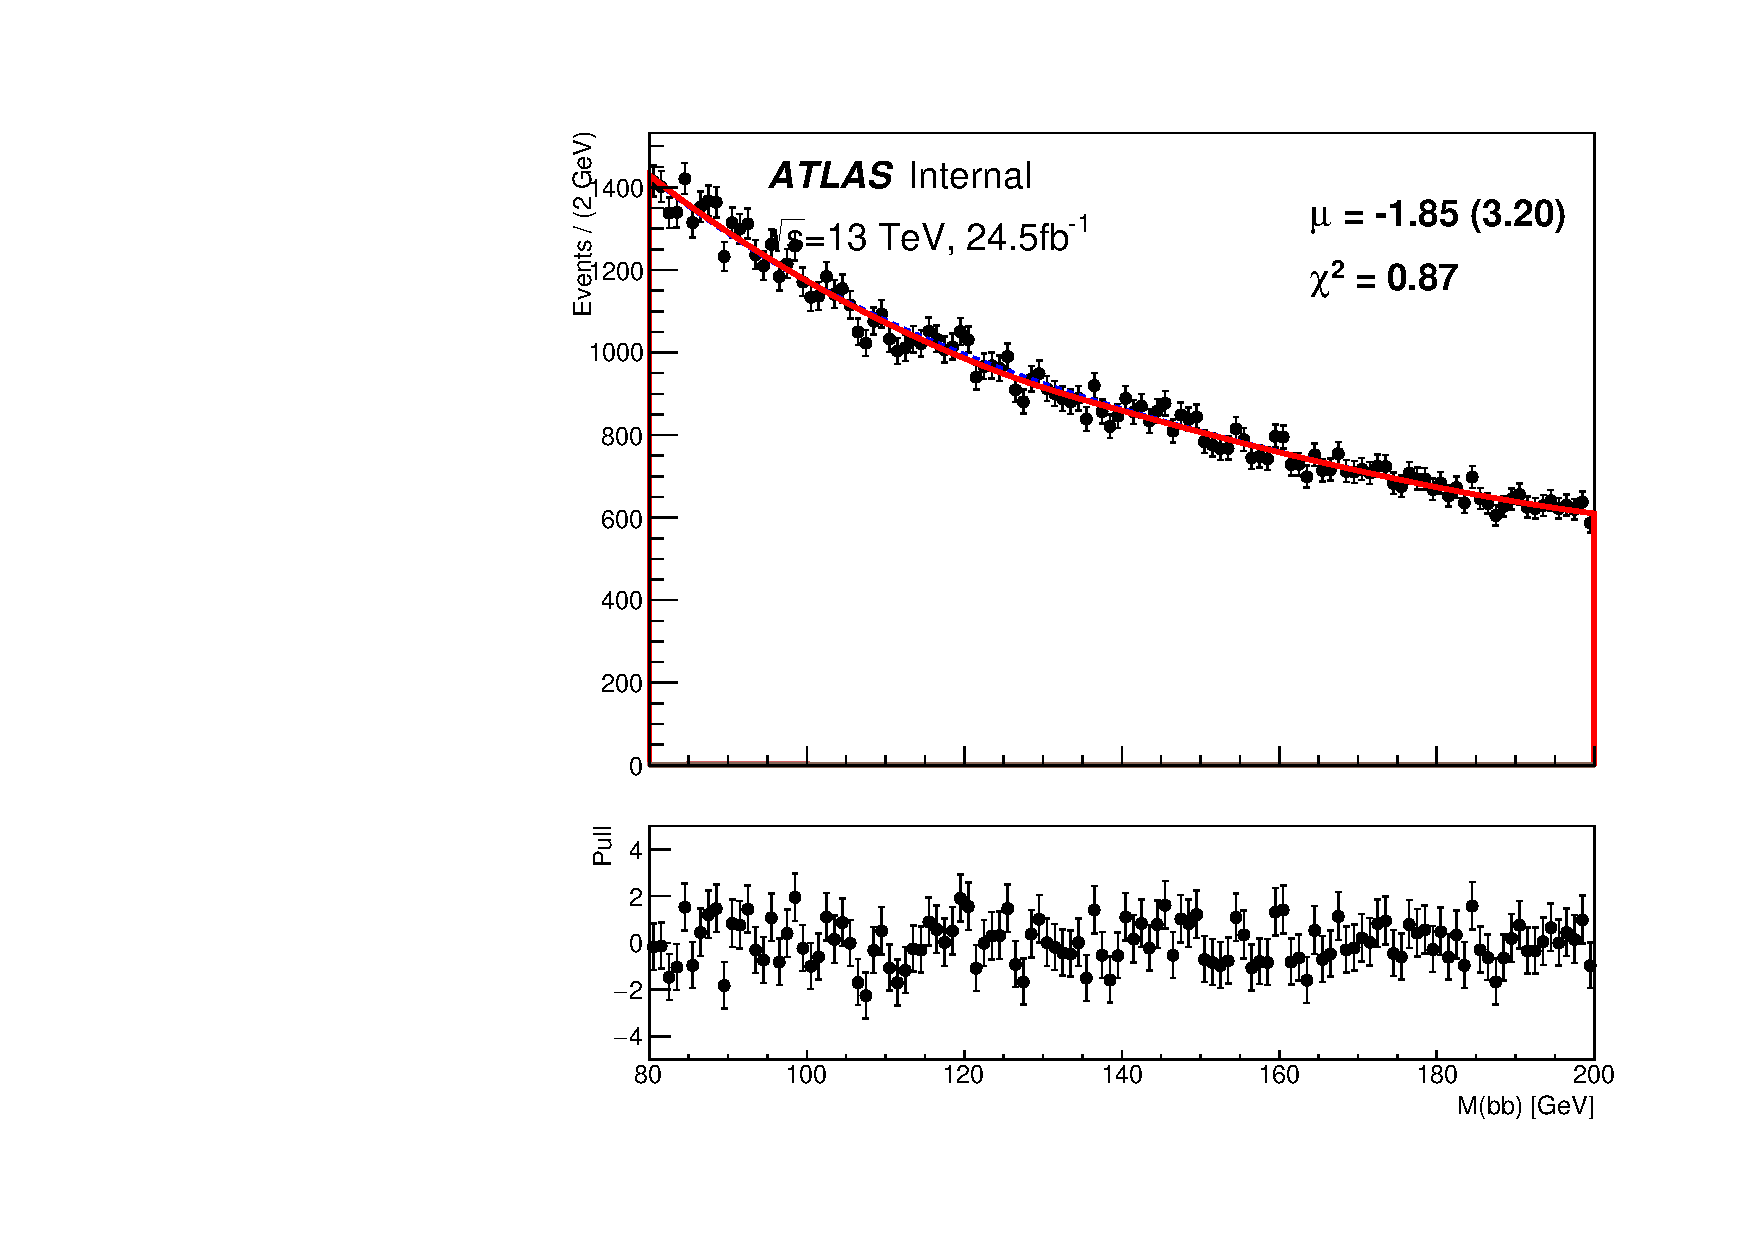
\includegraphics[width=0.24\textwidth]{figures/Fit2cen_SP/spurious_O4_testVBF_ICHEP_2cen_SRIII_CTRL.pdf}
 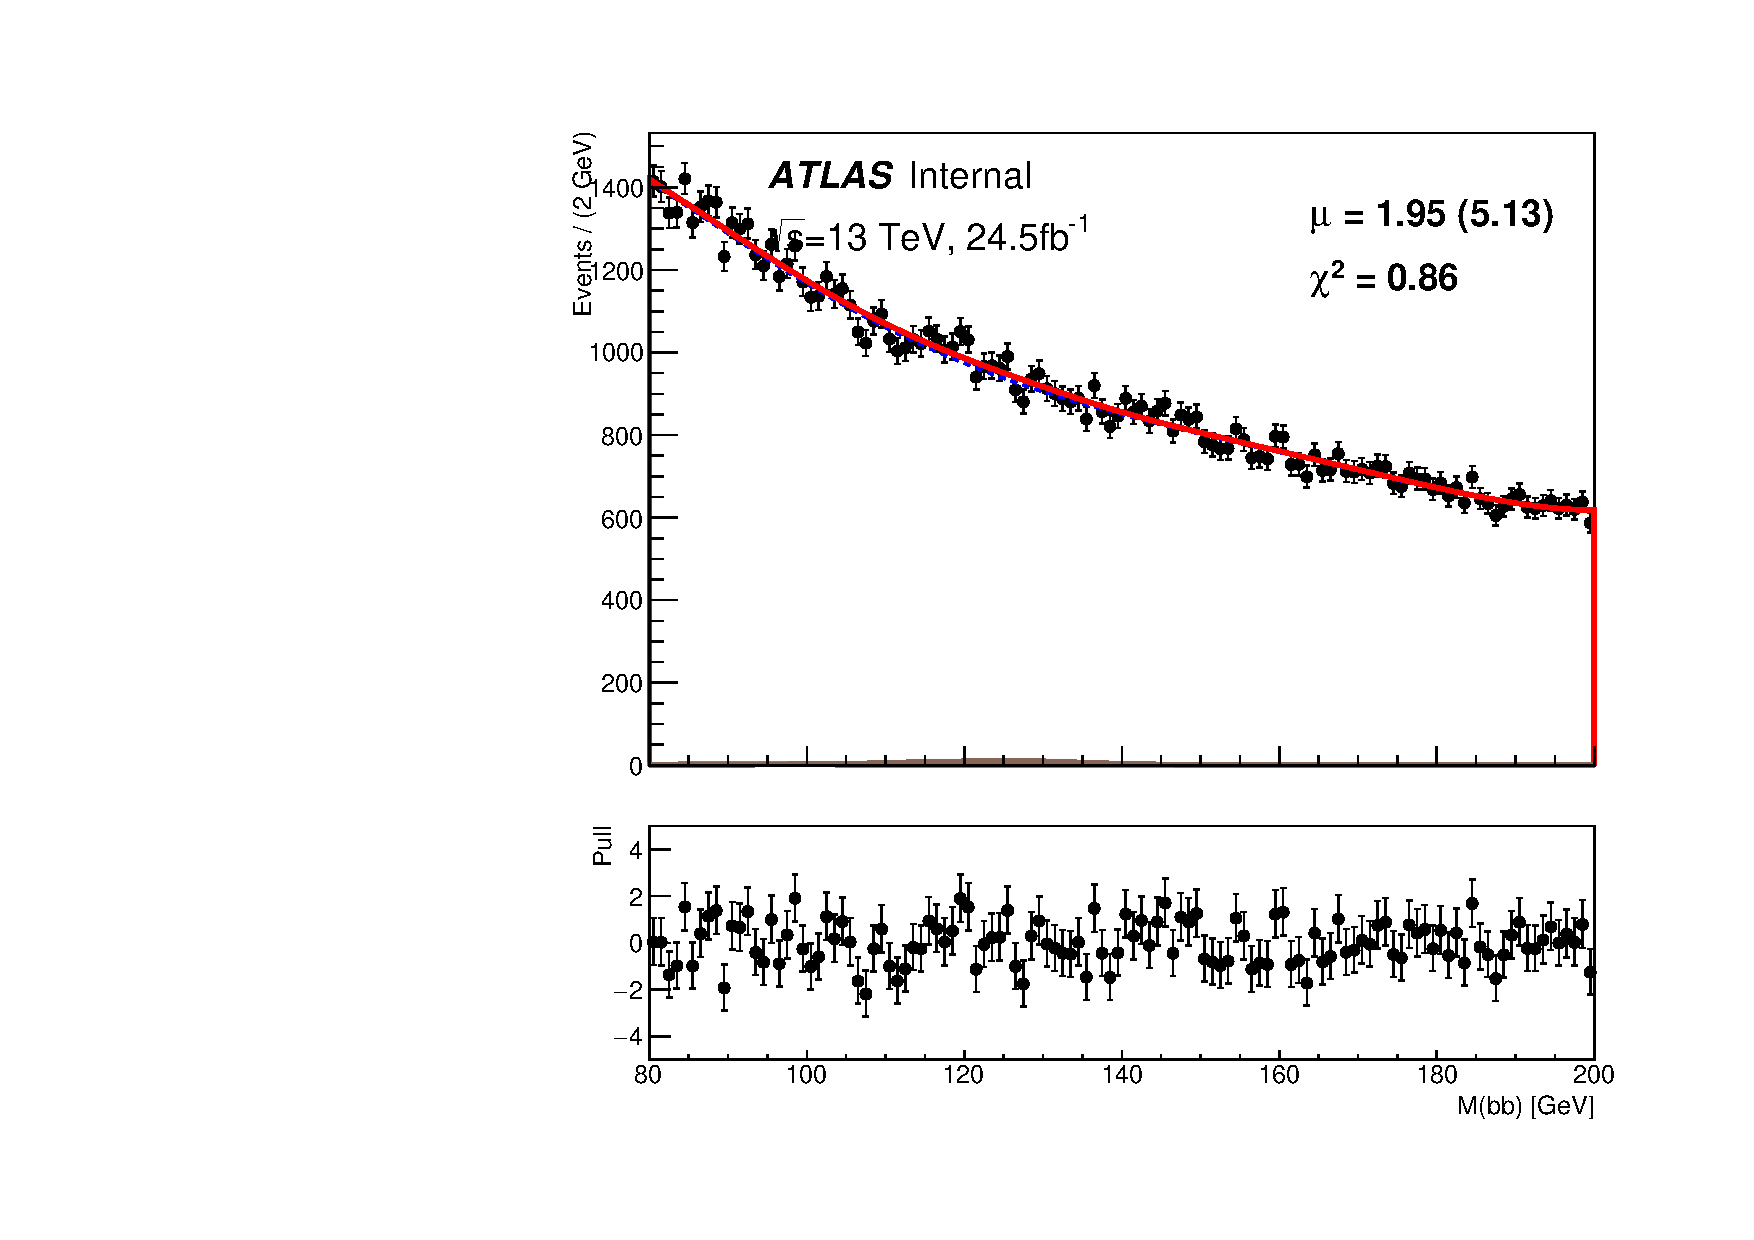
\includegraphics[width=0.24\textwidth]{figures/Fit2cen_SP/spurious_O5_testVBF_ICHEP_2cen_SRIII_CTRL.pdf}\\
\caption{Spurious signal fit for \twocentral channel in signal region I (top), II (middle) and III (bottom) with Bernstein O2 - O5 polynomials from left to right.  The bottom panel shows the pulls, defined to be $\frac{N_{\rm data} - N_{\rm fit}}{\sqrt{N_{\rm data}}}$ where $N_{\rm fit}$ includes the spurious signal. For all signal regions, the data in the Higgs mass window is taken from the control region and rescaled to match the normalization in the sidebands.}
  \label{fig:Fit_SP_2cen-old}
\end{figure}

\begin{figure}[htbp]
  \centering
 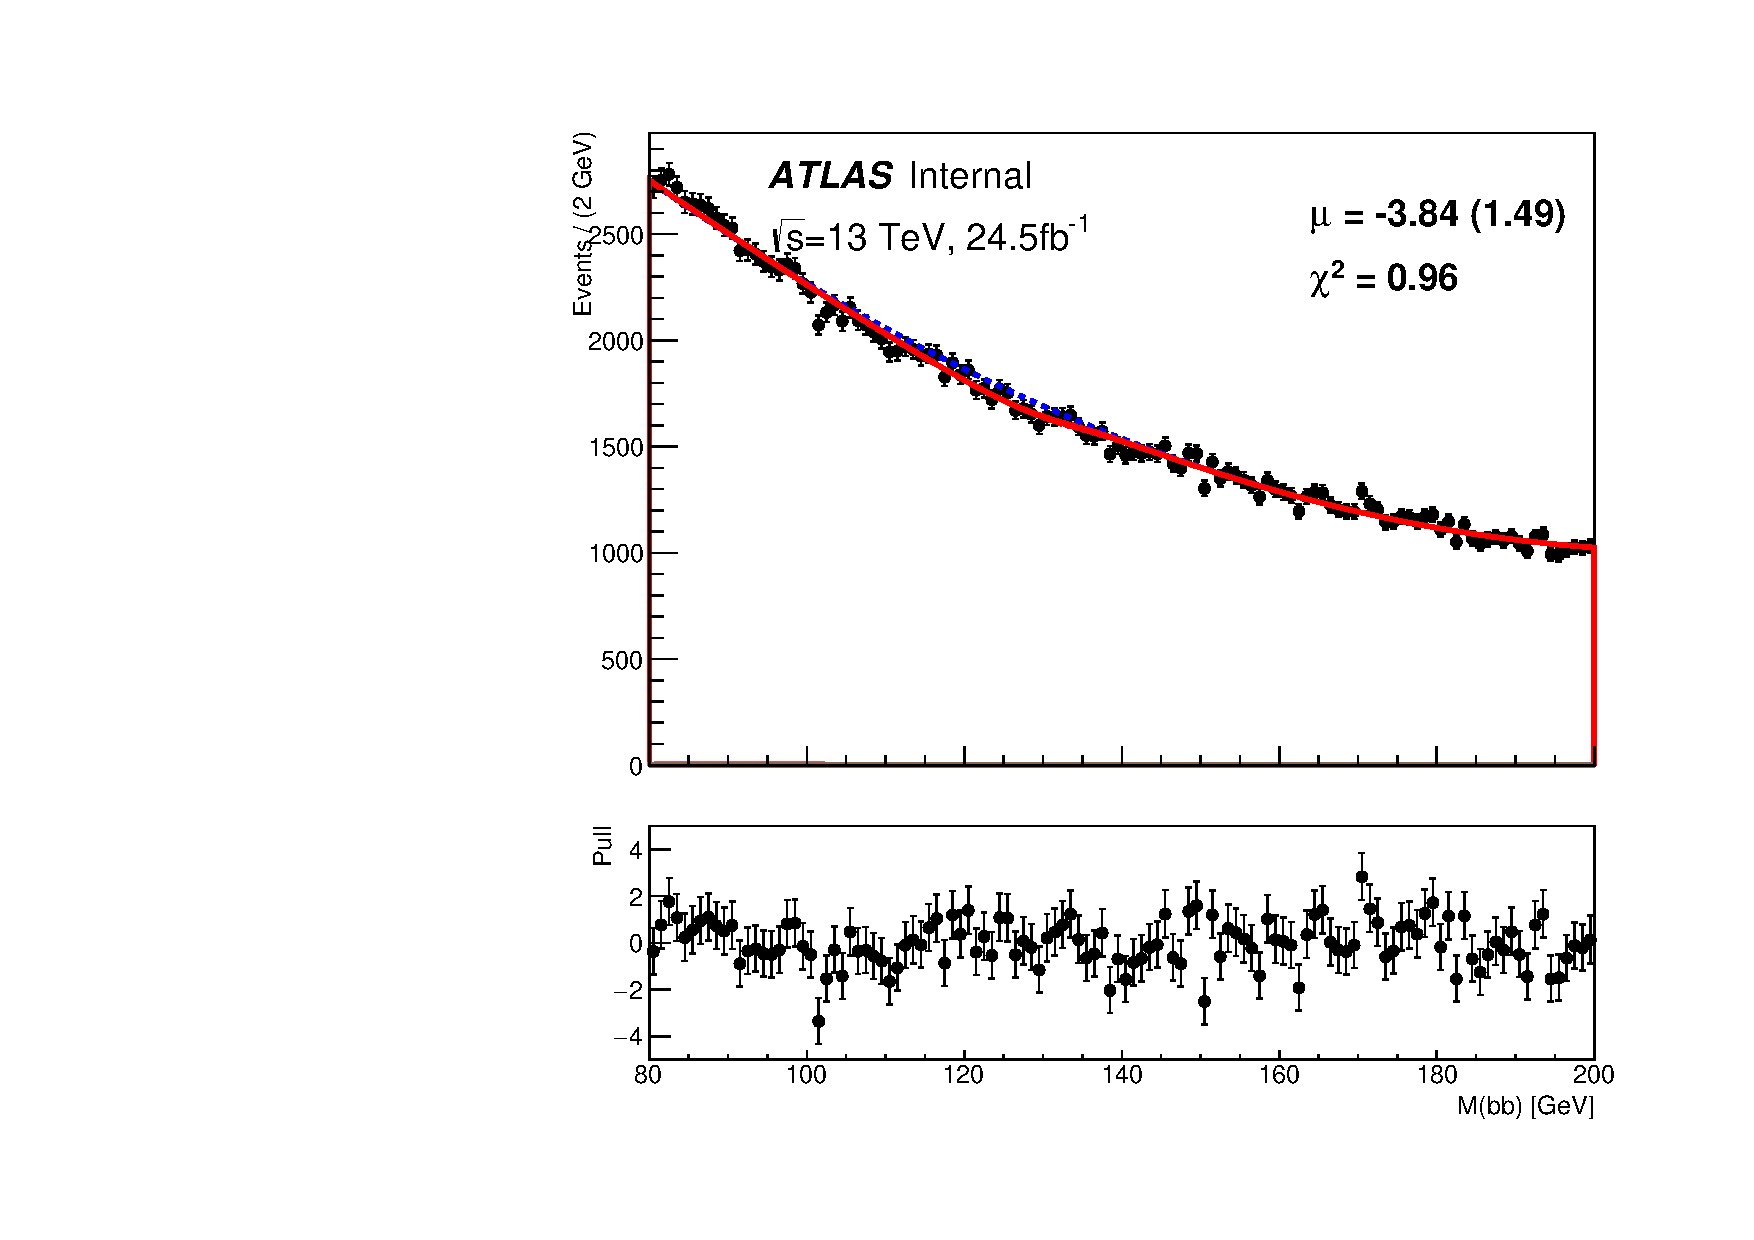
\includegraphics[width=0.24\textwidth]{figures/Fit4cen_SP/spurious_O2_testVBF_ICHEP_4cen_SRI_CTRL.pdf}
 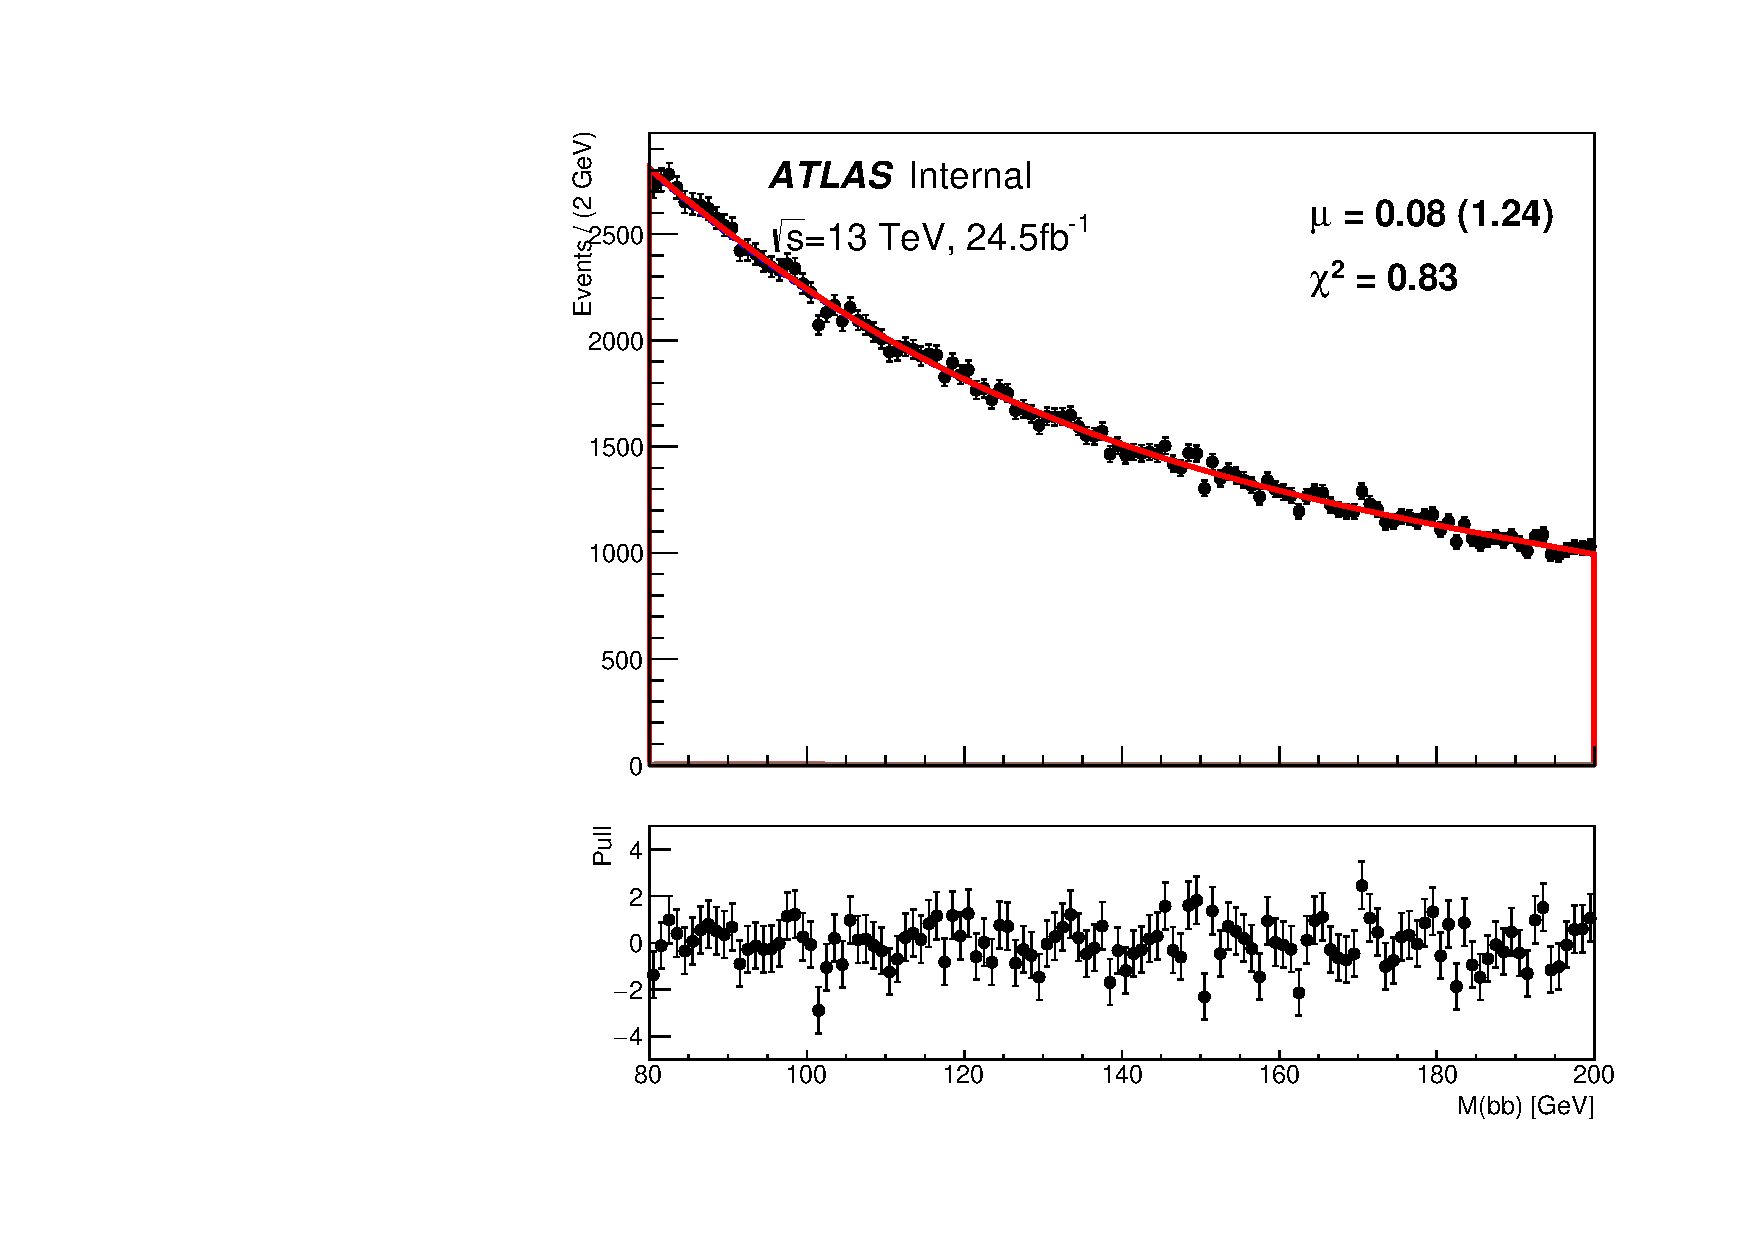
\includegraphics[width=0.24\textwidth]{figures/Fit4cen_SP/spurious_O3_testVBF_ICHEP_4cen_SRI_CTRL.pdf}
 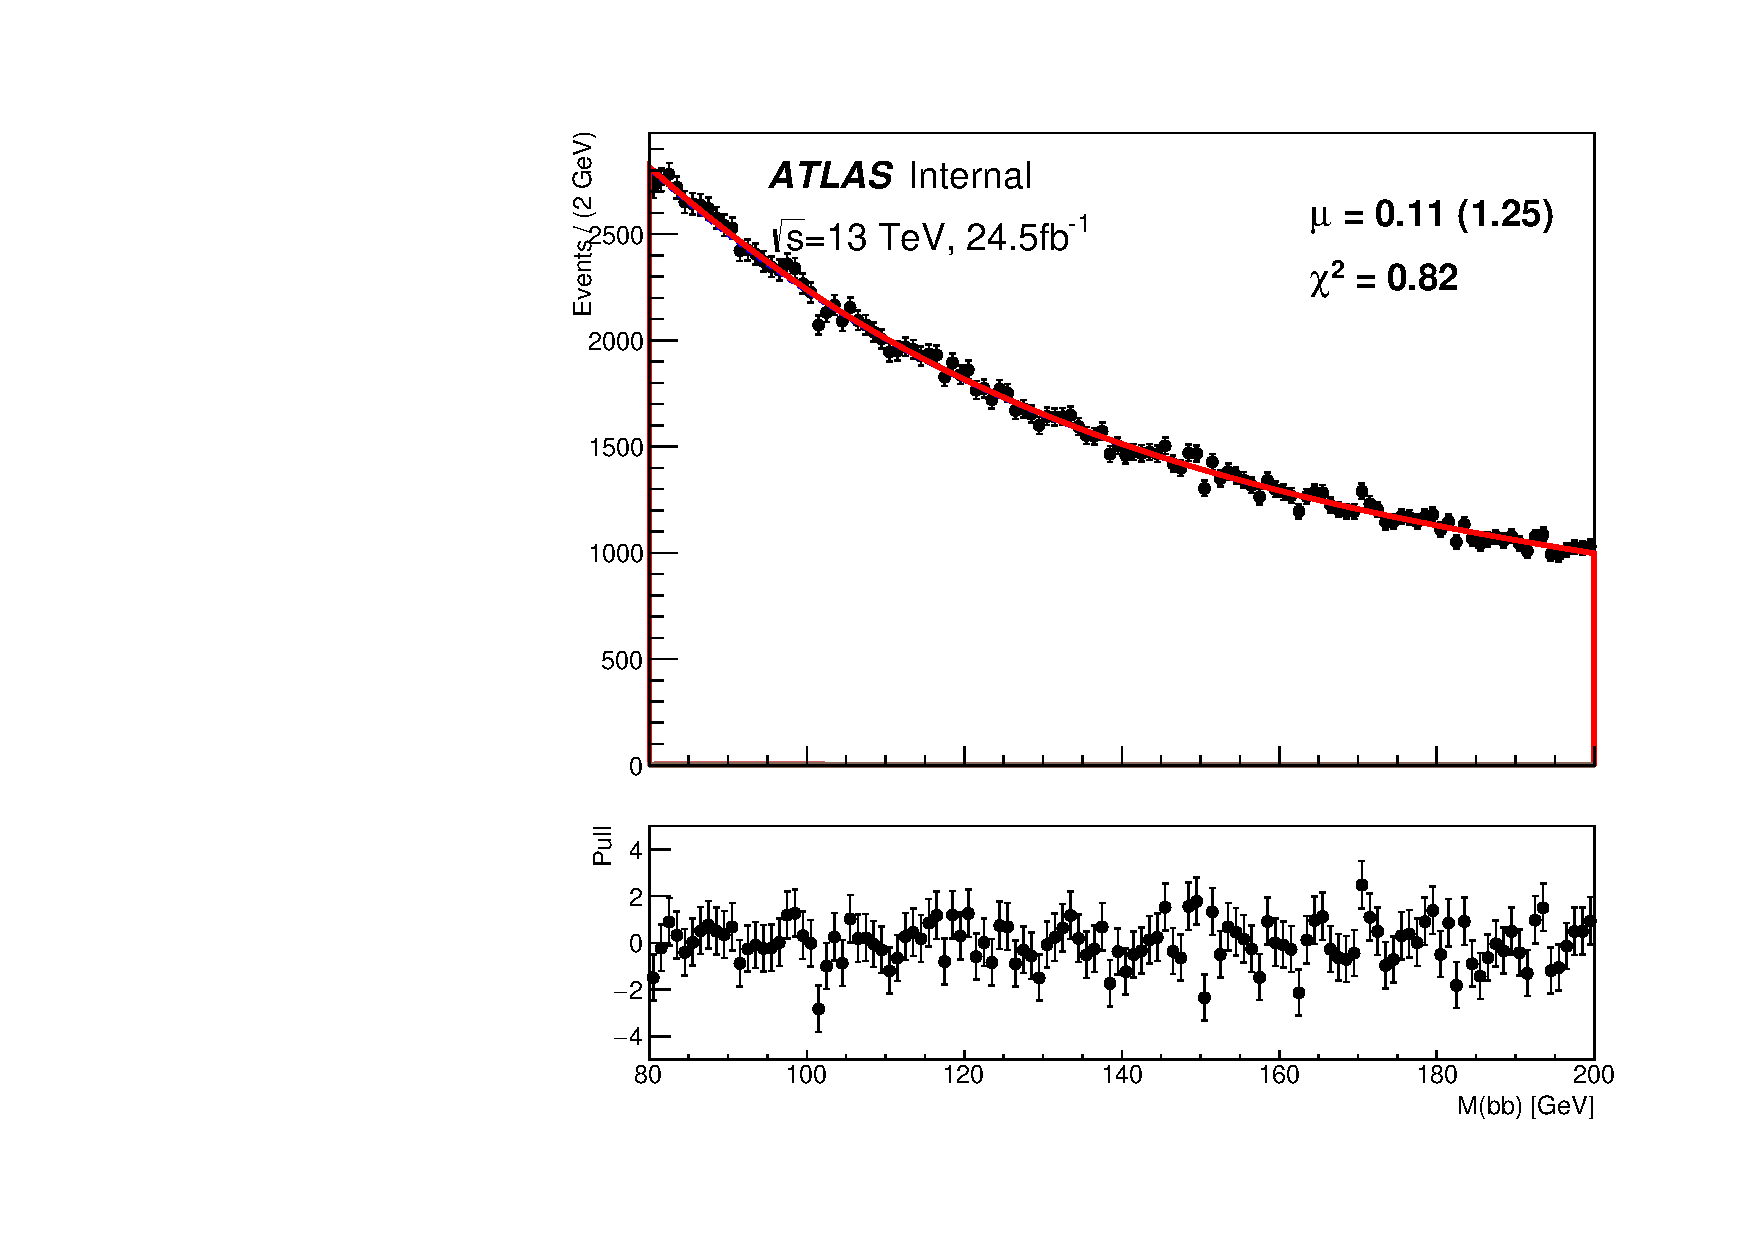
\includegraphics[width=0.24\textwidth]{figures/Fit4cen_SP/spurious_O4_testVBF_ICHEP_4cen_SRI_CTRL.pdf}
 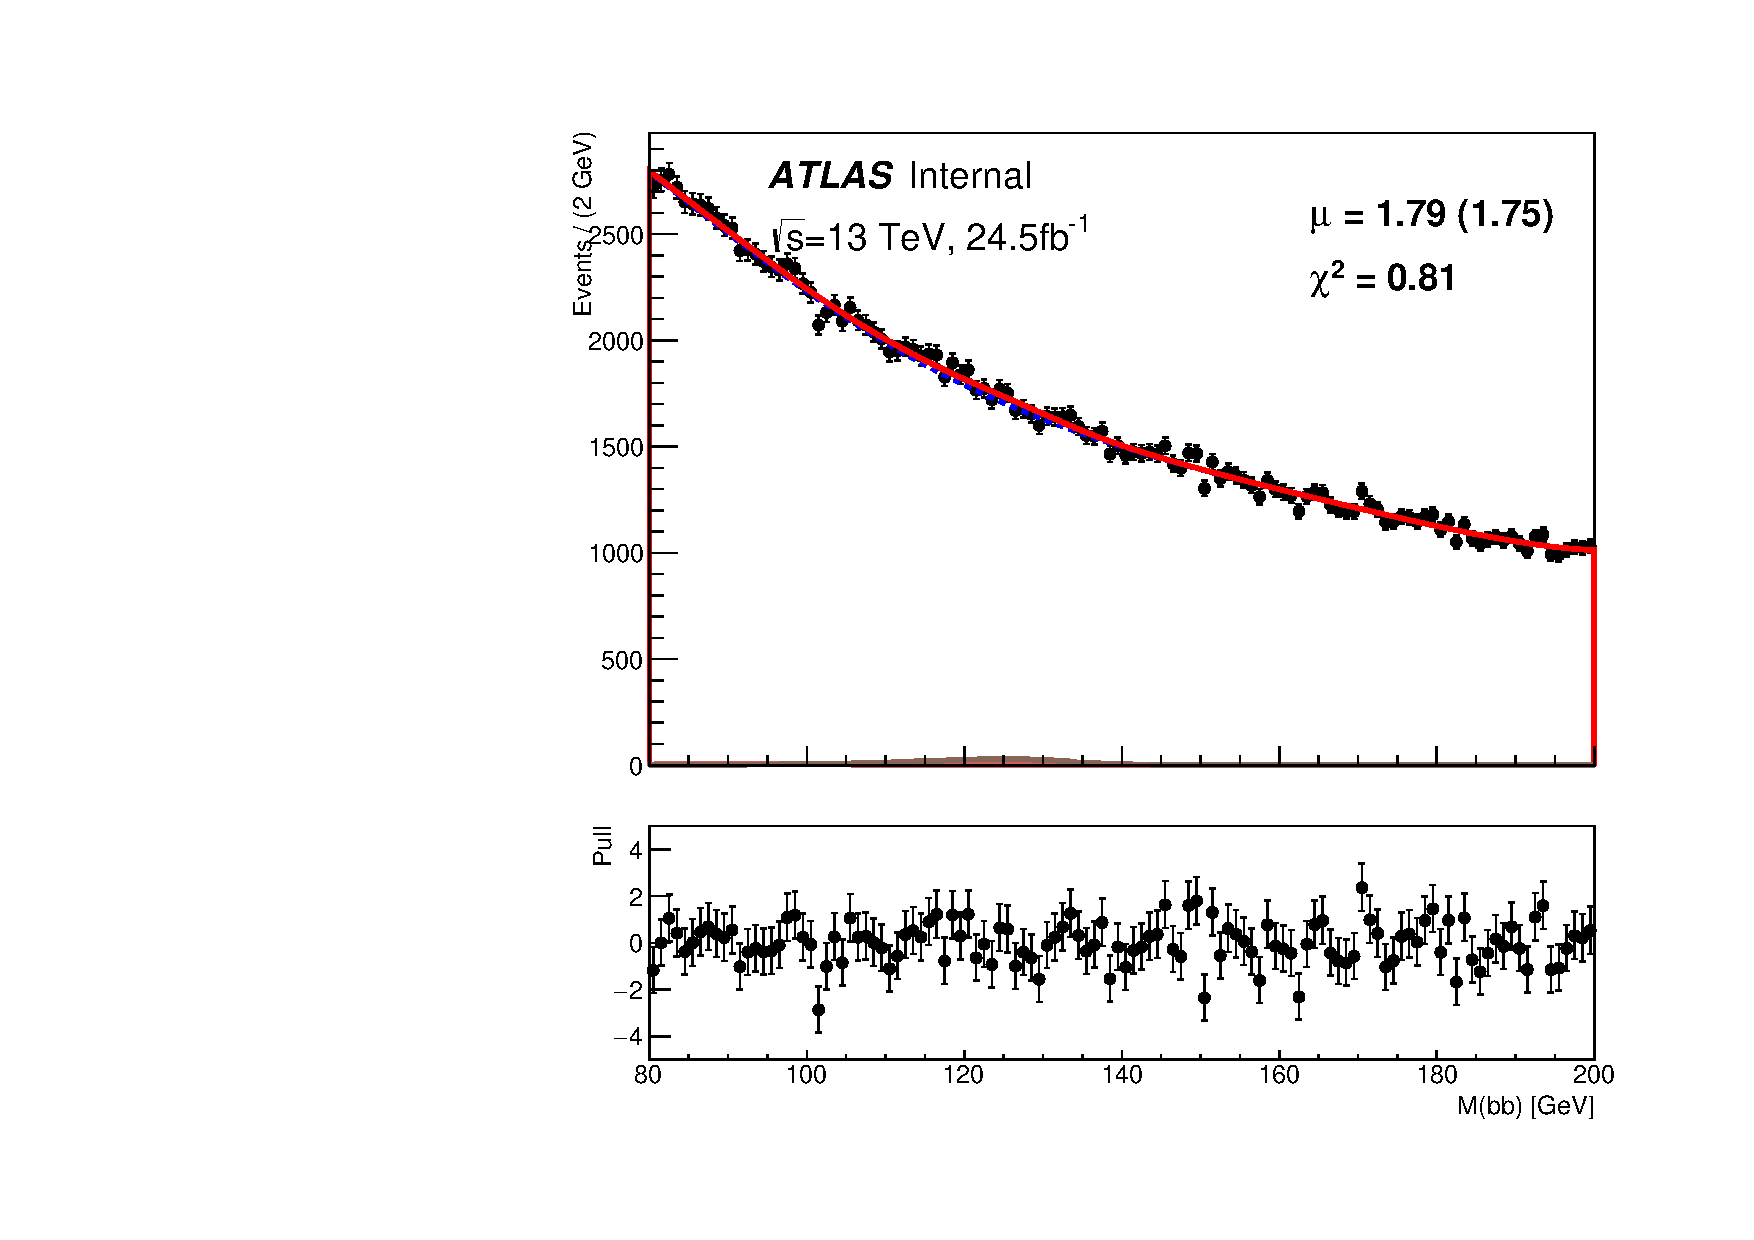
\includegraphics[width=0.24\textwidth]{figures/Fit4cen_SP/spurious_O5_testVBF_ICHEP_4cen_SRI_CTRL.pdf}\\
 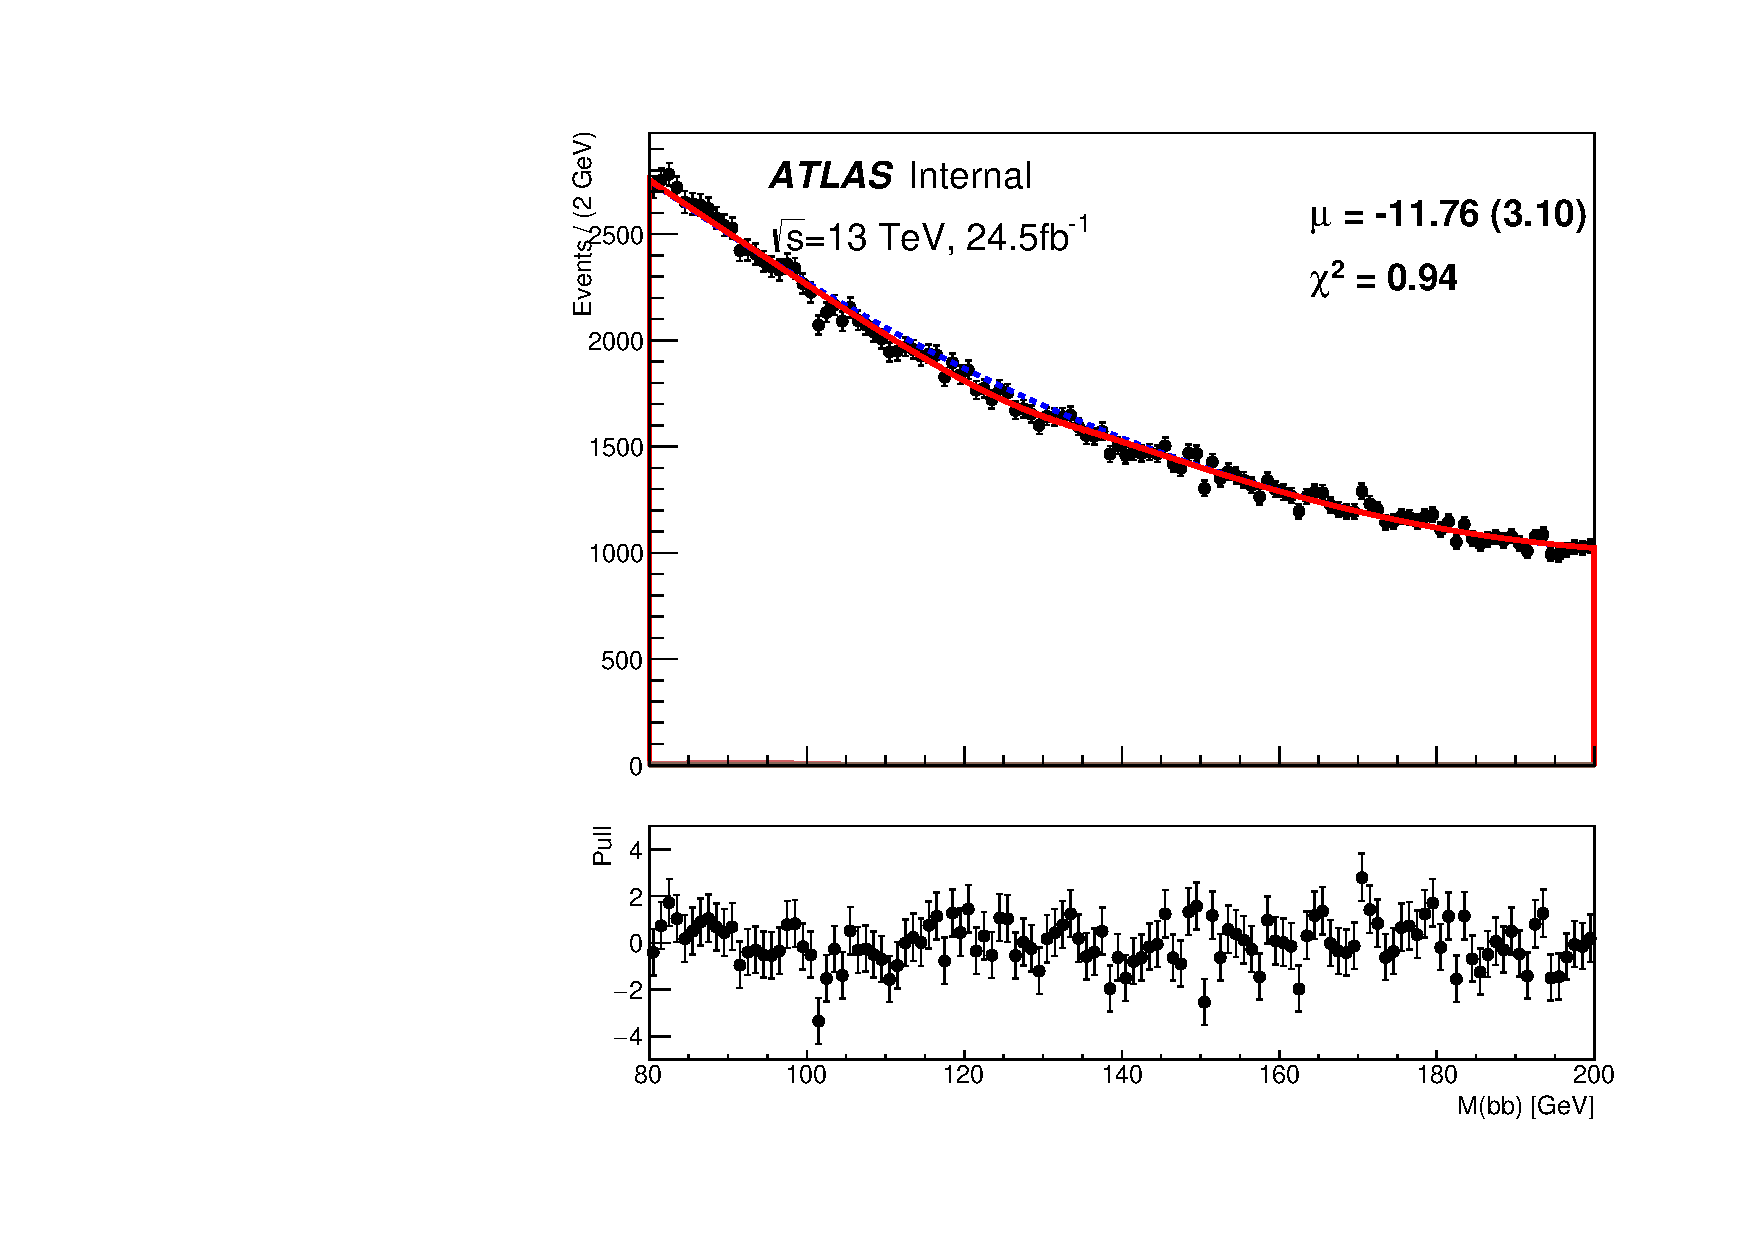
\includegraphics[width=0.24\textwidth]{figures/Fit4cen_SP/spurious_O2_testVBF_ICHEP_4cen_SRII_CTRL.pdf}
 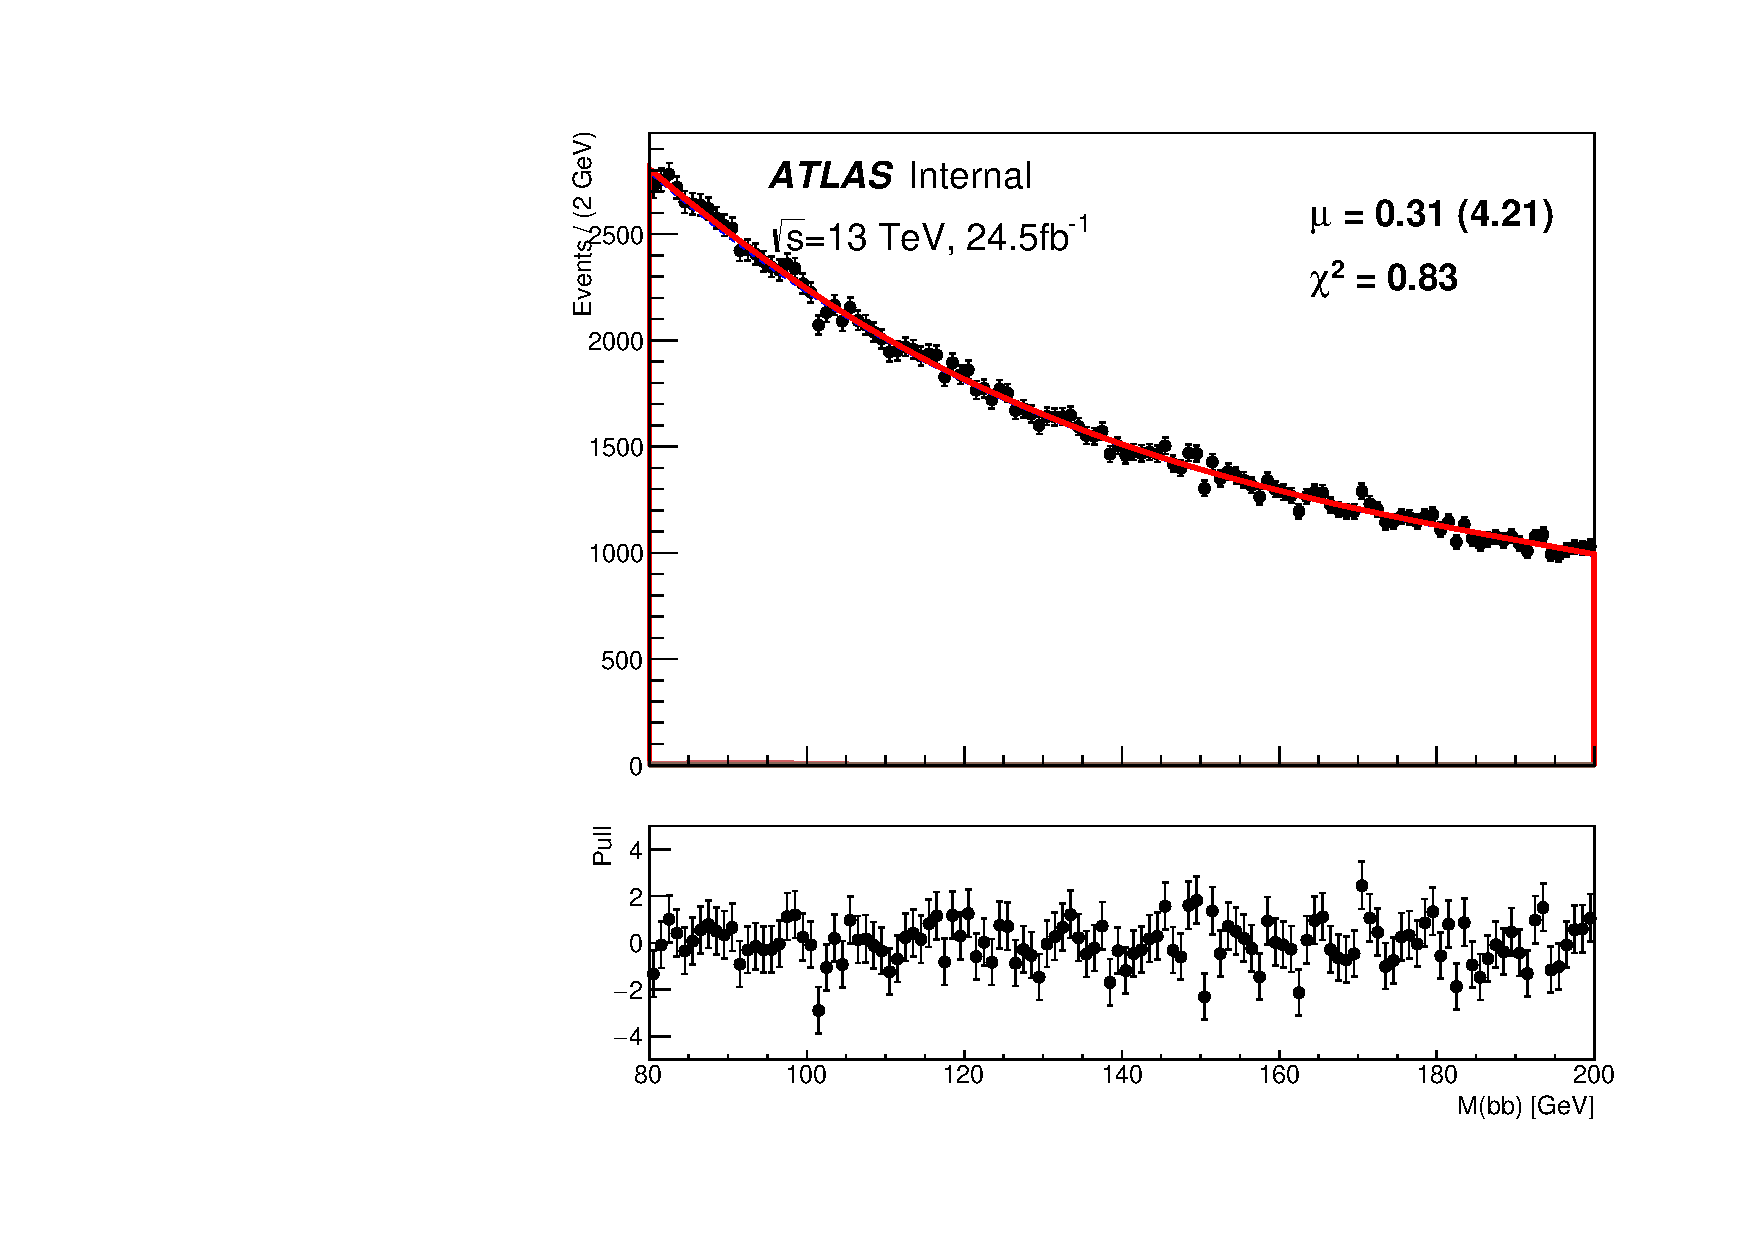
\includegraphics[width=0.24\textwidth]{figures/Fit4cen_SP/spurious_O3_testVBF_ICHEP_4cen_SRII_CTRL.pdf}
 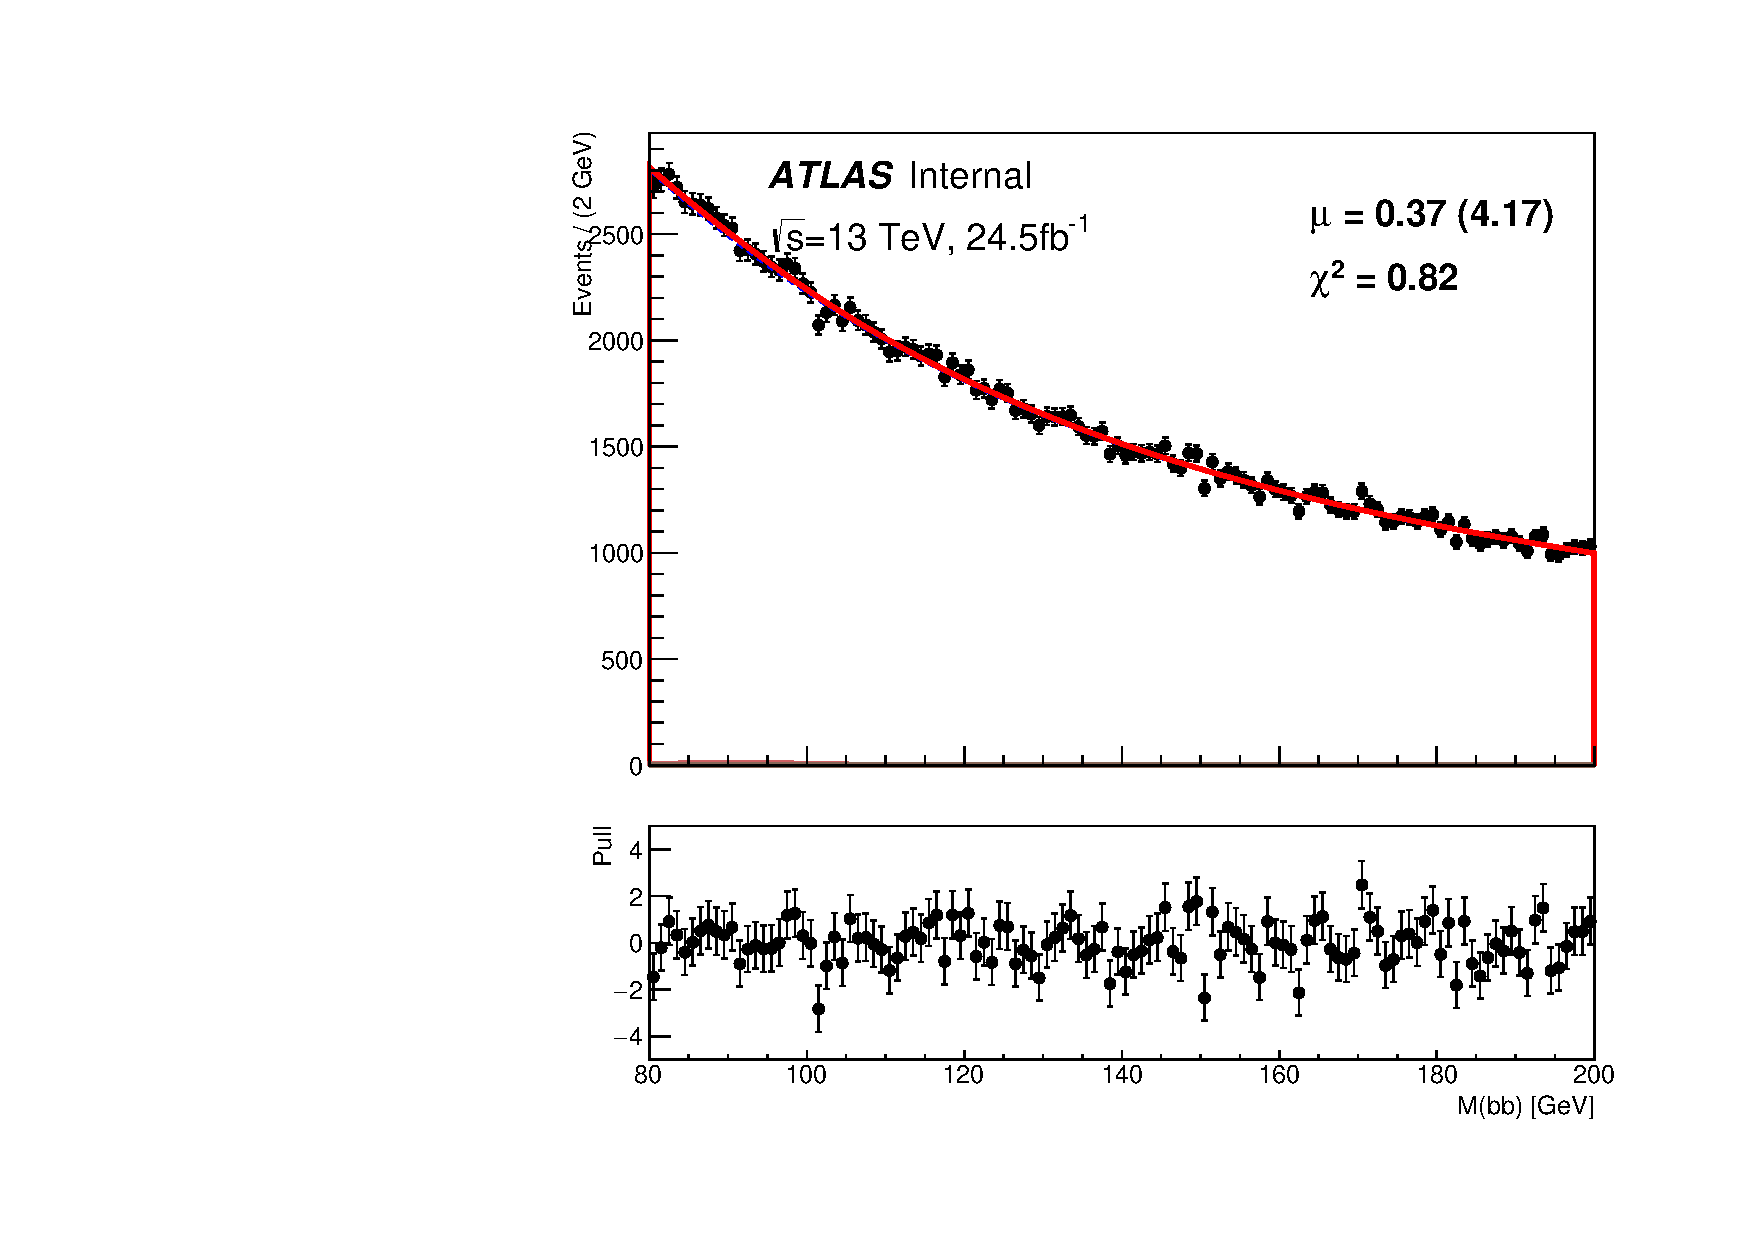
\includegraphics[width=0.24\textwidth]{figures/Fit4cen_SP/spurious_O4_testVBF_ICHEP_4cen_SRII_CTRL.pdf}
 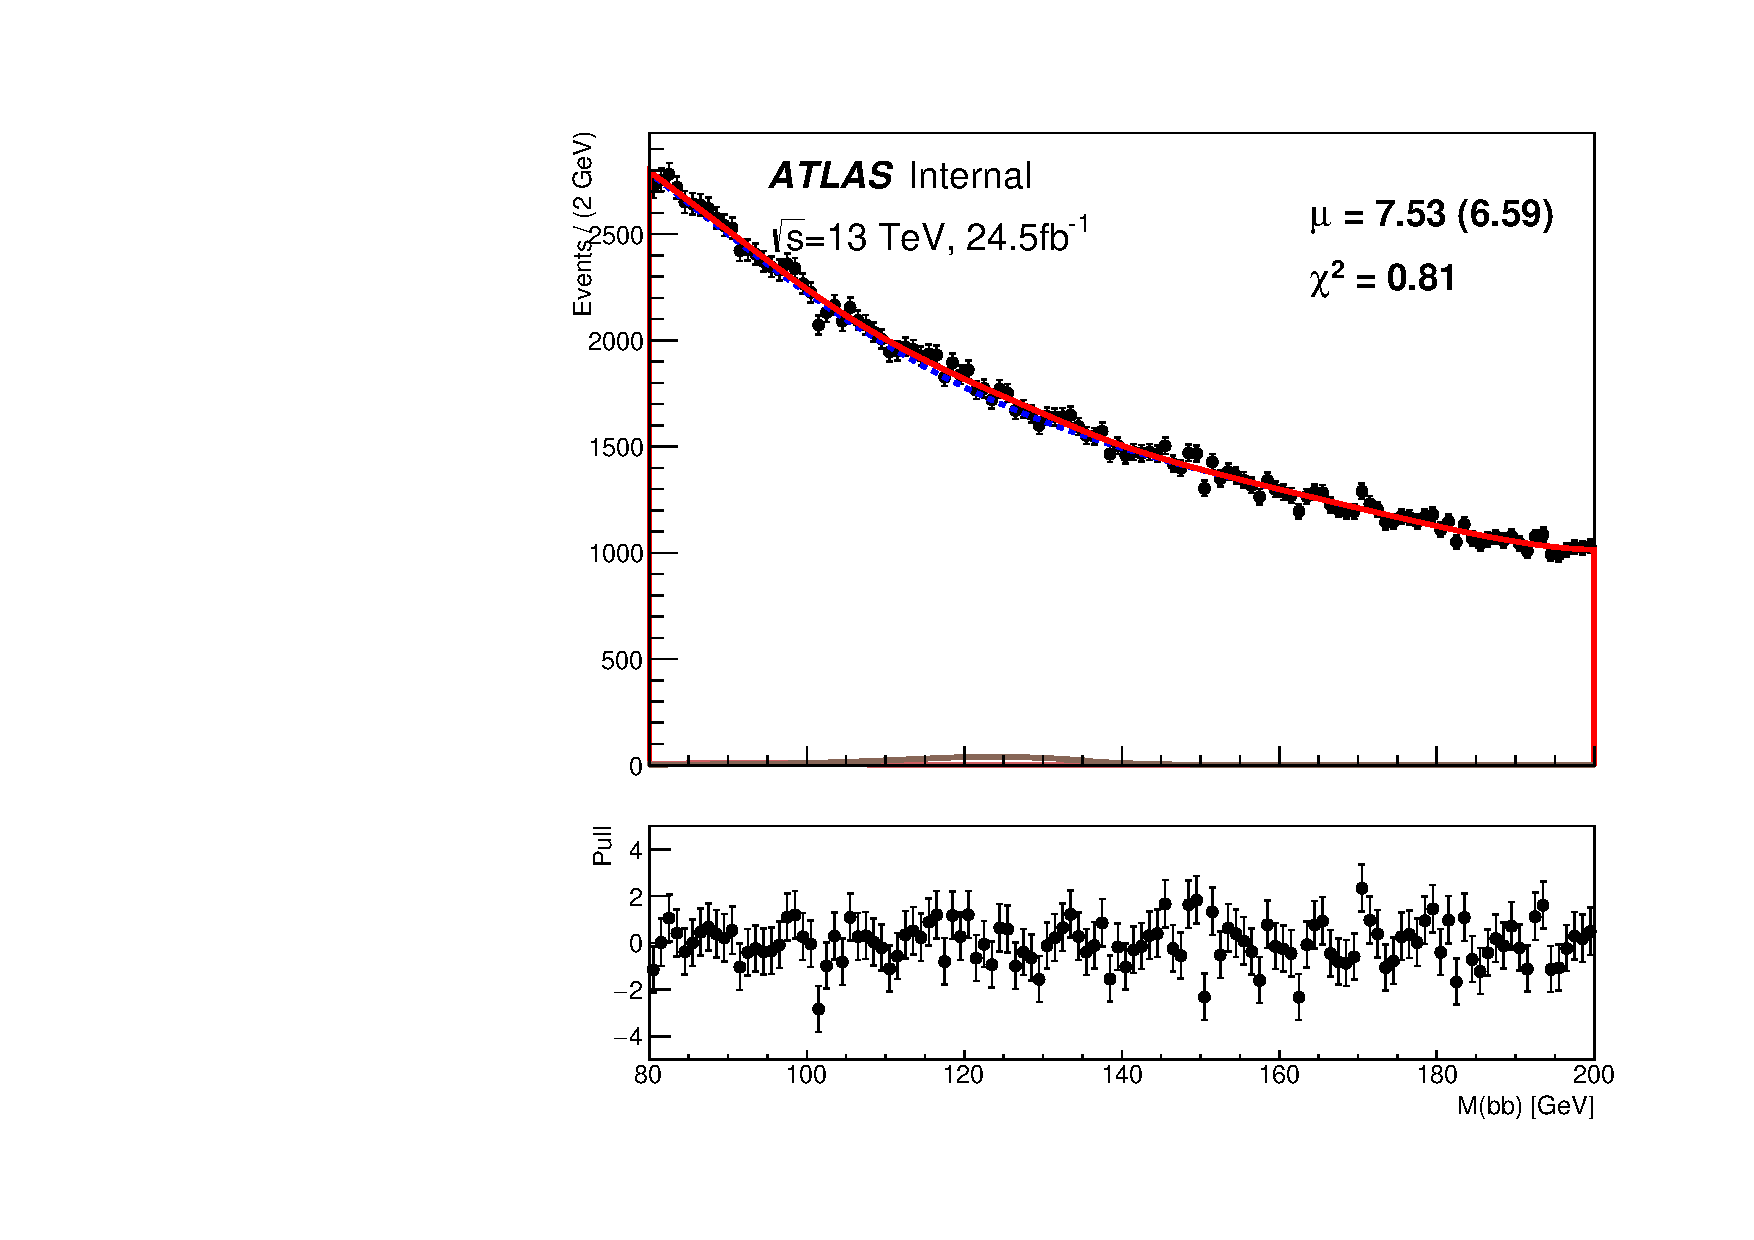
\includegraphics[width=0.24\textwidth]{figures/Fit4cen_SP/spurious_O5_testVBF_ICHEP_4cen_SRII_CTRL.pdf}\\
\caption{Spurious signal fit for the \fourcentral channel in signal region I (top) and II (bottom) with Bernstein O2 - O5 polynomials from left to right. The bottom panel shows the pulls, defined to be $\frac{N_{\rm data} - N_{\rm fit}}{\sqrt{N_{\rm data}}}$ where $N_{\rm fit}$ includes the spurious signal.}
  \label{fig:Fit_SP_4cen-old}
\end{figure}

\clearpage

\subsubsection{Treatment of \zjets{} contribution}
\label{sec:app-ztreat}

The \zjets{} contribution plays an important role in the overall fitting procedure due to the fact that it comprises a significant fraction lower \Mbb{} sideband ( 5--6(3--4)\% of the \fourcentral(\twocentral) selection) , yet the sideband does not extend to low enough \Mbb{} values to reliably constrain its contribution using the shape templates.  Therefore, the non-resonant background fit can be partially compensated by the $Z$-yield and vice-versa.  To mitigate the impact of this degeneracy, we could fix the contributions of \zjets{} in the fits to predictions from MC.  However, our \zjets{} MC is only leading order ($Z+$2 partons), and large or varying $k$-factors may be present in the different BDT regions.  However, we can compare \zmujets{} production in data and MC in order to determine the accuracy of modeling of the $Z$ contribution and  use the ratio of events in \zmujets{}  to \zjets{} MC to constrain the data to MC modeling.  
  %The jets in the \zmujets{} sample should have the same kinematic distributions as those the non-$b$ jets in the \zjets{} sample.  
%Therefore we can check the data to MC modeling of a relatively pure data  \zmujets{} sample, and  use the ratio of events in \zmujets{}  to \zjets{} MC to constrain the data to MC modeling.  

The details of the \zmujets{} selection and study are found in Appendix~\ref{sec:app-zmm}.  Cuts are applied to the dimuon $Z$-candidate to emulate the di-\bjet selection of the Higgs candidate.  The cross-section ratios of data to MC after pre-selection are calculated to be 0.74$\pm$0.1 and 0.79$\pm$0.1 for \twocentral and \fourcentral channels respectively.  The errors include the statistical uncertainties on the data and MC. The relative ratios of the number of events in data and MC, and between \zjets{} and \zmujets{} MC are shown in Table~\ref{tab:z_ratios-old} for all of the regions considered in the analysis.  Large deviations from 1 are seen for many of the ratios.  Notably the \zmujets{} to \zjets MC ratio is not close to one in some regions, which may be due to the fact that different generators are used for the electro-weak production events, or due to residual differences in the \bjet and muon events arising from a different mis-tag rate and different final state QCD radiation effects.

Due to limited \zjets{} MC statistics, we do not take the product of the ratio of data to MC \zmujets{} events and the ratio of the \zmujets{} to \zjets{} to correct the \zjets{} MC prediction.  Instead, we use the data to MC ratio of \zmujets{} as the overall normalization factor with a  single gaussian nuisance parameter with a width equal to the uncertainty on the ratio.  Then in each BDT region the cross-section is scaled to the ratio of $\frac{Z\rightarrow \mu \bar \mu(Data)}{Z\rightarrow \mu \bar \mu(MC)}$ and we adopt one nuisance parameter per region.  The width of this parameter is the uncertainty on the ratio as derived from the data and MC statistics.   

%What we do instead is take the ratio \zmujets/\zjets as nuisance parameter on the  overall $Z$ normalization factor and use the difference between the two in MC as the uncertainty.  The overall Z normalization is taken from data.  Then, each individual BDT region normalization is scaled to the \zmujets{} data/ MC ratio with no uncertainty.



\begin{table}[]
\centering
\caption{Relative Ratios of $Z\rightarrow \mu \bar \mu$(Data) to \zjets{}(MC) in each BDT region}
\label{tab:z_ratios-old}
\begin{tabular}{|l|r|r|}
\hline
Region       &  $\frac{Z\rightarrow \mu \bar \mu(Data)}{Z\rightarrow \mu \bar \mu(MC)}$ & $\frac{Z\rightarrow b \bar b(MC)}{Z\rightarrow \mu \bar \mu(MC)}$   \\ \hline
SRI (2cen)   & 0.82 (0.15) & 0.43 (0.12)\\ \hline
SRII (2cen)  & 0.42 (0.13) & 0.35 (0.14)\\ \hline
SRIII (2cen) & 0.61 (0.11) & 0.91 (0.17)\\ \hline
CR (2cen)    & 1.26 (0.11) & 1.26 (0.13)\\ \hline
SRI (4cen)   & 0.74 (0.05) & 0.64 (0.07)\\ \hline
SRII (4cen)  & 0.80 (0.03) & 0.86 (0.05)\\ \hline
CR (4cen)    & 1.47 (0.07) & 1.40 (0.09)\\ \hline

\end{tabular}
\end{table}


%We have evaluated the Z(mumu)+jets yield in data and MC for the various BDT regions.  Unfortunately, the Zbb and Zmumu MC have very little statistics in the SR1.  This is not surprising because, again, this is a rather weird corner of phase space.   Nonetheless, the comparison between the relative Z(mumu) and Z(bb) yield in MC, together with the Z(mumu) data yield, gives an ?envelope" of predictions (Ideally, we would use Z(bb,MC)*Z(mumu, data)/Z(mumu,MC) and propagate the uncertainties, but we don?t have Z(bb) and Z(mumu) decayed from the same MC events, therefore this would amplify the already large statistical fluctuations).  What we do instead is take the ratio Z(mumu, data)/Z(mumu,MC) as nuisance parameter on the  the Z normalization factor and use the difference between the Z(mumu) to Z(bb) MC as the uncertainty {LT NOTE: This seems a bit strange to me ? let?s talk about it.}  	Then, each individual BDT region normalization is scaled to the Z(mumu) Data/ MC ratio with no uncertainty


\subsection{Uncertainties}
\label{sec:uncertainties-old}
The treatment of the uncertainties are unchanged from the main text.
%-------------------------------------------------------------------------------
%\label{sec:vbf-uncertainties}

Several sources of systematic uncertainties,
affecting the normalization of signal and background and/or the shape of
the distributions used in this analysis, have been considered.  Individual sources of systematic 
uncertainty are considered uncorrelated. The systematic variations with less than $0.5\%$ impact 
on the yields in a particular BDT region will be ignored in the profile likelihood fit for 
that particular region. 

\subsubsection{Luminosity}
\label{sec:vbf-syst_lumi}

The integrated luminosity measurement has an uncertainty of 3.4\%. This systematic uncertainty
is applied to all physics processes estimated with MC simulated samples normalized 
to the measured integrated luminosity: \zjets{} and Higgs production. {\it Ed. Note: this will be updated after the unblinding.}

\subsubsection{Uncertainties on object definitions}
\label{sec:vbf-syst_objects}

Several uncertainties are applied to the MC simulation samples to take into account the limited knowledge of the detector and reconstruction performance.

\paragraph{Trigger efficiencies}

The per-jet online b-tagging efficiency with respect to the offline b-tagging efficiency is measured in $t\bar t$ events. 
To cover the event topology dependence, a scale factor applied to the leading b-tagged jet is derived as a function of the jet $\eta$. 

\paragraph{JVT efficiency}
The per-jet efficiency to satisfy the jet vertex tagging requirement
is measured in $Z(\to \ell^+\ell^-)$+1-jet events in data and simulation,
selecting separately events enriched in hard-scatter jets and events enriched in pile-up jets. 
The corresponding uncertainty is evaluated by shifting the per-jet scale factors,
accounting for the efficiency uncertainty~\cite{JVTwiki}.

\paragraph{Jet energy scale}
%\label{sec:vbf-syst_jes}
The jet energy scale and its uncertainty have been derived combining information from test-beam data, 
LHC collision data and simulation \cite{JESwiki}. The jet
energy scale uncertainty is split into 4 uncorrelated sources, 
which can have different jet $\pt$ and $\eta$ dependencies.  These sources are
treated independently in this analysis, using the \texttt{JetUncertainties} tool \cite{TWiki_JetUncertainties} 
to compute the uncertainties corresponding to each eigenvector. 
The variation in the jet energies as a result of these systematic uncertainties are also propagated through all
observables computed using jet kinematics.

\paragraph{Jet energy resolution}
%\label{sec:vbf-syst_jer}
[The jet energy resolution (JER) has been measured separately for data and simulation 
using in-situ techniques. The \texttt{JERUncertaintyProvider}
tool~\cite{jeruncertaintyprovider} was used to obtain the expected fractional
$p_T$ resolution for a given jet as a function of its $p_T$ and rapidity. 
The systematic uncertainty is taken by smearing the jet energy by the shift 
in resolution provided by the tool and comparing to the nominal
shape and normalization in simulation. 
The nominal value is used as the default in the analysis.

In order to propagate the uncertainty in the $p_T$ resolution, for each jet a 
random number $r$ is drawn from a Gaussian distribution with mean 0 and sigma equal 
 to the difference in quadrature between the fractional $p_T$ resolution with the tool and the nominal
one.  The jet 4-momentum is then scaled by a factor $1+r$.  By definition, such uncertainty
is one-sided, since jets in simulation cannot be under-smeared. 
We compute the normalization and shape uncertainties in the final distributions 
and symmetrize them to define a corresponding "down'' variation.

\paragraph{\btagging}
%\label{sec:vbf-syst_btag}

The effects of uncertainties in efficiencies for the heavy flavor tagging of jets by
the MV2c10 tagger have been evaluated. This analysis uses the operating points 
with approximately 60\%, 70\% and 85\% efficiency for $b$-quark jets. 
These efficiencies are measured
from data for each jet flavor.

Simulation efficiencies for $b$ and $c$ quarks have to be corrected by a
$\pt$-dependent factor. In the case of light flavor jets, the corrections also 
depend on jet $\eta$. 
Each uncertainty corresponds to a resulting eigenvector after diagonalizing the matrix
containing the information of total uncertainty per $\pt$ bin and the bin-to-bin 
corrections. These systematic
uncertainties are taken as uncorrelated between $b$, $c$, and light flavor jets.
A per-jet weighting procedure is applied to simulated events to propagate the 
calibration of $b$-tagging and the related uncertainties. 
The correlation across operating points is ignored. It has been checked that this choice
wouldn't impact the results by considering the uncertainties fully correlated or fully uncorrelated.


\paragraph{Track multiplicity for Quark/gluon separation}

The track multipicity discrimination power for quark/gluon separation in simulation 
is affected by the modeling of the charged multiplicity in jet fragmentation and the modeling of the
track multiplicity reconstruction. The estimation of the corresponding uncertainties is 
described in Ref.~\cite{qgtagging}. A total of 5 nuisance parameters is used to parametrize these
uncertainties and the impact on the results presented in this note is found to be negligible.

\subsubsection{Analytical and Theoretical Modeling uncertainties of signal}
\label{sec:vbf-syst_model}

Uncertainties in the modeling both of the non-resonant background shape and the theory and phenomenological modeling uncertainties of the Monte Carlo simulation samples are described here.


\paragraph{Non-resonant background}
The non-resonant background is modeled with an analytical function, either O(3) or O(4) Bernstein polynomial. 
The potential local bump or dip caused by the functional choice is characterized by spurious signal 
which is derived by fitting the nominal model plus signal to an alternative model. The derived spurious signal 
size is then quoted the width of a gaussian constraint which is included in the profile likelihood as in 
Eq.~\ref{likelihood}.

%\paragraph{\zjets{} normalization}
%\label{sec:vbf-zjets}
%
%Strategy~\label{item:z-treat-5} of section~\ref{sec:vbf-ztreat} is taken for the systematic uncertainties on the \zjets{} normalization.
%
%The bias on the signal $\mu$ value caused by this rescaling (or lack thereof) is estimated 
%with an injection test where the scaled pseudodata is fit with the non-scaled template. 
%The bias is found to be less than $10\%$ and therefore negligible with respect to the overall uncertainty.
%Therefore no relative rescaling is applied to the \zjets{} MC prediction in each region.
%Additional details of these studies are provided in Appendix ~\ref{sec:vbf-app-zmm}.

%The normalization of the \zjets{} background, simulated at LO, is 
%affected by potentially large uncertainties~\cite{zkfactors}. 
%In order to estimate the \zjets{} normalization in data, the $Z(\mu\mu)+$jets yield
%is used as proxy. The ratio between data and MC yield after preselection is used to estimate the overall
%normalization and the difference between \zjets{} and $Z(\mu\mu)+$jets is 
%taken as uncertainty.
%The data/MC ratio is found to be 0.74(0.1) and 0.79(0.1) for \twocentral and \fourcentral channels respectively. 
%A single gaussian NP with width 0.1 is therefore used in the global fit. 
%The $Z(\mu\mu)+$jets sample is also used to study the variation across signal and control regions.
%The \zjets{} prediction is scaled in each BDT region by the ratios between the yields observed in $Z(\mu\mu)+$jets data
%and in \zjets{} and $Z(\mu\mu)+$jets MC. The scale factors are listed in Table~\ref{tab:z_ratios}
% 

\paragraph{QCD Scale Variations}

The QCD scale uncertainty for VBF is taken as varying the renormalization
and factorization scales together by a factor of 2 and 0.5. As indicated in ~\cite{QCDscale_vbf}, 
this treatment in general leads to larger variations than the independent variation of renormalization
and factorization scales. 

The QCD scale uncertainty for ggF follows the \textit{2017 scheme} recommended by 
WG1 in the follow-up of March meeting 2017 ~\cite{QCDscale_ggF}. In total, nine independent 
variations in six categories are considered. The terms and corersponding uncertainty sources 
are the following:

\begin{enumerate}
\item \textit{mu}, factorization scale variation
\item \textit{res}, renormalization scale variation
\item \textit{vbf2j} and \textit{vbf3j}, VBF topology uncertainties
\item \textit{mig01} and \textit{mig12}, truth level bin migration for non-Higgs jets
\item \textit{pTH60} and \textit{pTH120}, uncertainties extrapolation with Higgs $p_T$
\item \textit{qmt}, uncertainties of top quark mass
\end{enumerate}

The dominant source of uncertainty for this analysis comes from the term \textit{mig12} (size of $~17-18\%$), 
which is the leading source of uncertainty in high $p_T(H)$ event topology. 

Naively, one would assume uncertainties due to VBF topology terms are considerable. 
However, it is worth noting that these terms only matter for events which 
at truth level are generated in VBF topology. An event falls into Stage one classification 
of VBF topology if the truth Higgs has $p_T<200GeV$ and 
\begin{enumerate}
\item $MJJ>400 GeV$ and $|\textnormal{rapidity(J1)-rapidity(J2)}|>2.8$ ( loose VBF, events having >3 jets),
\item Pass loose VBF selection $\overrightarrow{p_{T}}(J1)+\overrightarrow{p_{T}}(J2)+\overrightarrow{p_{T}}(Higgs)<25GeV$ (tight VBF, events having ~2 jets),
\end{enumerate}
where the VBF jets are defined as the leading two jets aside from the Higgs. We note that $80\%$ of the events have $p_T(H)>200GeV$ and 
these events would not fall into the VBF category. Hence, the VBF topology uncertainties would not even apply in the \textit{2017 scheme} for most of our events. 
For our application, we could extend the definition of VBF topology to high $p_T(H)$ events and take the \textit{vbf2j} and \textit{vbf3j} values
for low $p_T(H)$ VBF topology to be the uncertainty for high $p_T(H)$ events as well. (\textit{vbf2j} and \textit{vbf3j} are defined as constants.)

We also notice that the \textit{2017 scheme} has a different definition of VBF jets, which selects the leading two jets aside from Higgs,  from the 
offline selection we apply in this analysis, which seeks a pair of jets that maximizes the $MJJ$ value. Hence if an event which is categorized by \textit{2017 scheme}
as non-VBF, the scheme lacks a term to properly count the 2J VS. 3J truth event topology uncertainty. Therefore, we also propagate the VBF topology 2J VS. 3J
uncertainties to standard non-VBF ggF+GE2j category. 

Overall, if VBF topology uncertainties are only applied to low $p_T(H)$ events, this source 
of ucnertainty is $<3\%$ in all signal regions. If the uncertainty is extended to high $p_T(H)$ events and as well as non-VBF ggF+GE2j events, the uncertainty
is about $20\%$. We take this conservative extended version of uncertainty for ggF events.

%\begin{table}[htbp]
%\centering
%\caption{Fraction of ggF events in high $p_T(H)$ and VBF topology category}
%\label{tab:highpTfraction}
%\begin{tabular}{|l|l|l|l|l|l|l|}
%Region   & 2cen SR I & 2cen SR II & 4cen SR I & 4cen SR II & 4cen SR III & 4cen SR IV \\
%Fraction & 17.5\%    & 10.4\%     & 13.2\%    & 19.4\%     & 8.8\%       & 9.5\%     
%\end{tabular}
%\end{table}


\paragraph{PDF}
The uncertainty on the PDF description used to simulate the signal is evaluated
by varying the PDF based on the uncertainties along each of the PDF eigenvectors.
Each variation is applied by reweighting the signal samples event-by-event.
A single nuisance parameter, corresponding to the envelope of all the variations,
is considered.

\paragraph{Parton Shower}

The modeling of parton shower could directly affect observables which are heavily 
correlated with the jettiness of the event. In this analysis, its impact is most 
prominent on $p_{T}$ balance, which is a variable used as the BDT input. The nominal
Pythia sample is compared with the \herwig{} sample at the truth level to derive a 
reweighting map for $p_{T}$ balance.
This reweighting map is then applied to the observable of the reconstructed events. The full impact of this variation 
is evaluated by running the BDT analysis while fixing other variables at their nominal 
and applying reweighting of $p_{T}$ balance. 


\paragraph{Signal Contamination from \VH and \ttH Processes}

The cross section of other Higgs production mode like \VH and \ttH are comparable to
the VBF process. Events from \VH (fully hadronic final states) and \ttH production could 
also pass the event selections of this analysis. The \Mbb distributions of these process
 are shown in Figure~\ref{fig:Mbb-ttH-VH}. The yields of these processes are presented 
in Table~\ref{tab:vh-tth-yield}.  The contributions to the total Higgs yields are  small 
in the most sensitive signal regions (0.2 -- 0.8 \%),  and rise to 15\% in the least sensitive regions.  

The VH process has a prominent resonance peak, similar to the VBF and ggF distributions. However, 
the statistics of the Monte Carlo sample is low, especially in \twocentral channel. 
We assign a 100\% uncertainty to the \VH process yield for a conservative estimate of 
the \VH contribution. %Its yield is added to the Higgs yields from VBF and ggF processes.

The \ttH mass distribution is a combination of the resonance peak and a continuum. 
The continuum arises from the fact that the \ttH process has at least four $b$-jets in the final state.
The failure of the jet assignment to identify the correct Higgs daughter $b$-jets results in a 
continuum combinatorial background which can be clearly seen in Figure~\ref{fig:Mbb-ttH-VH}. 
The yield is also assigned with 100\% uncertainty.
%In the fit, we take the actual shape of \ttH treating it as a background. 


\begin{figure}[htbp]
  \centering
 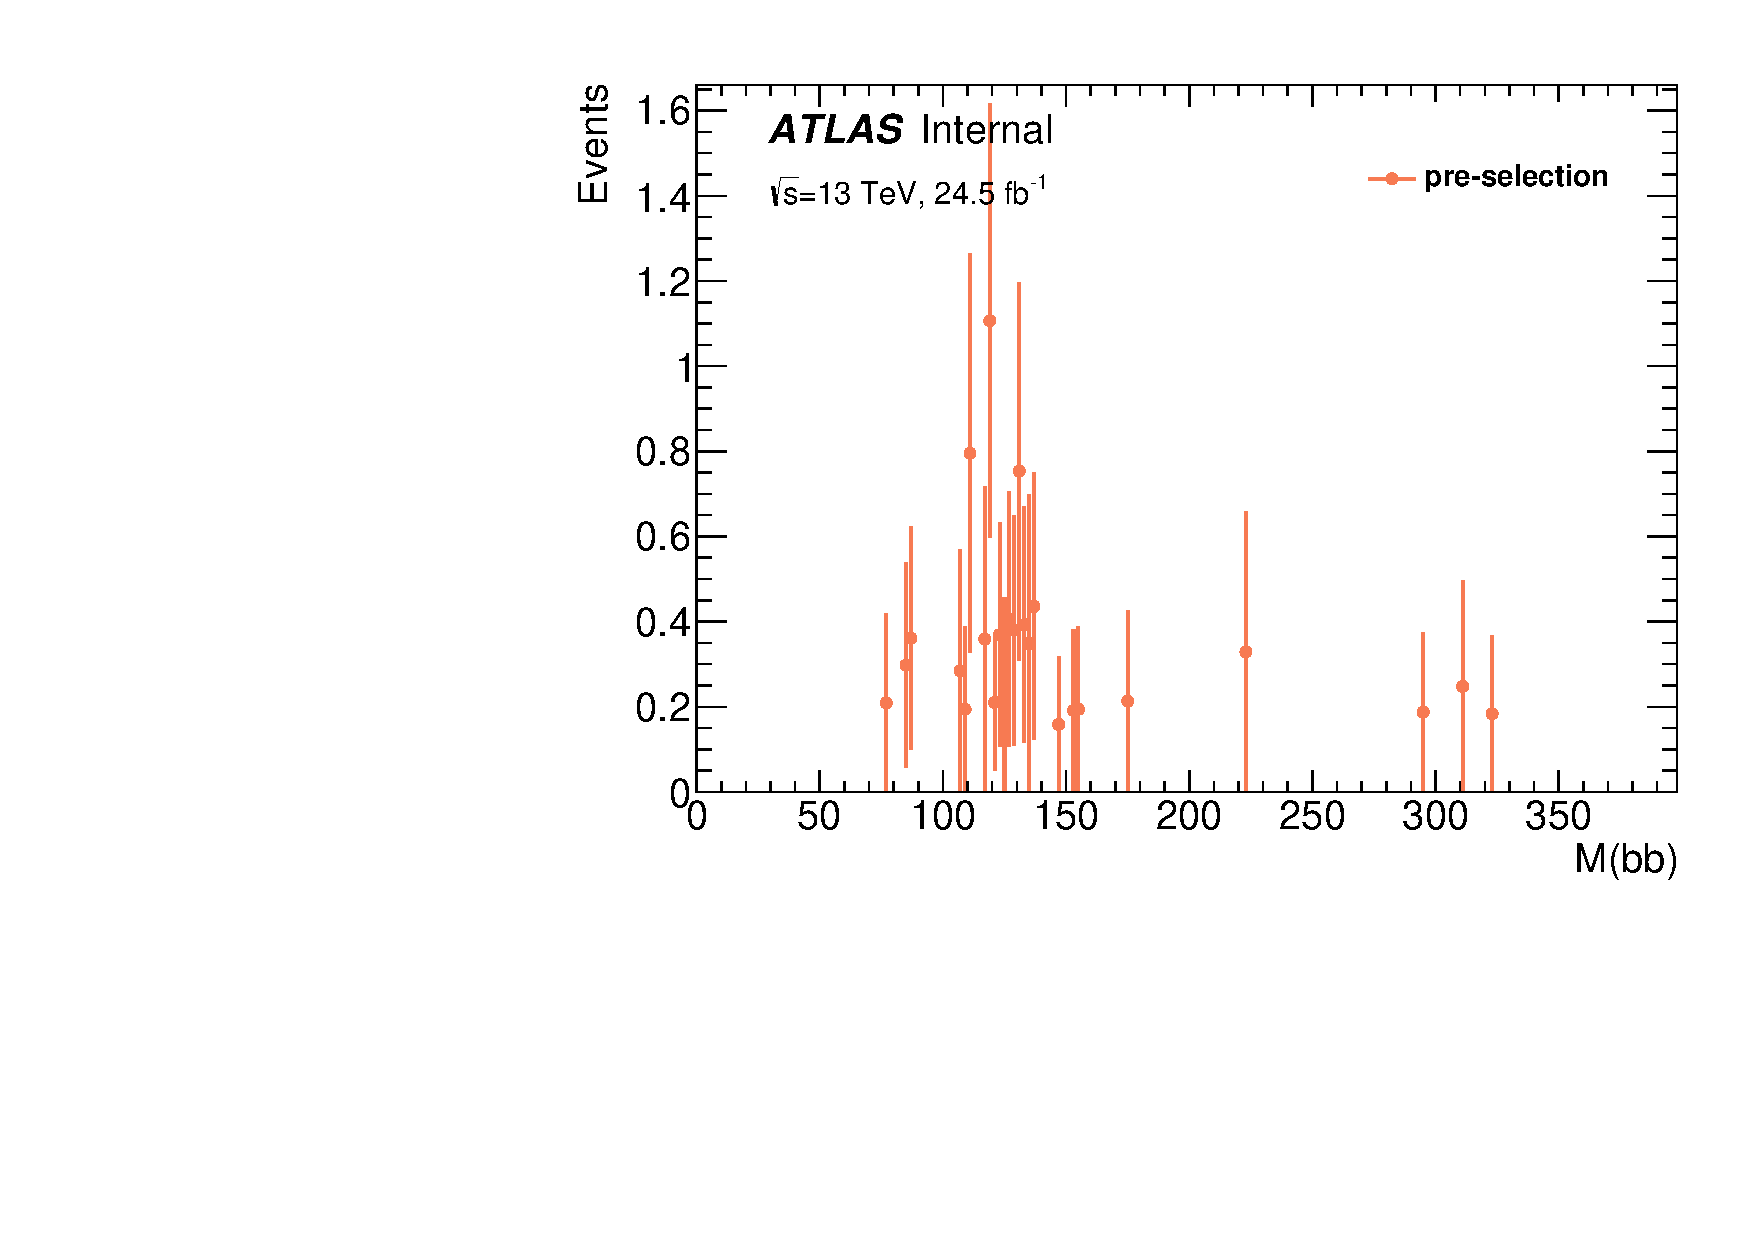
\includegraphics[width=0.42\textwidth]{figures/VBF/Mbb_VH_2cen.pdf}
 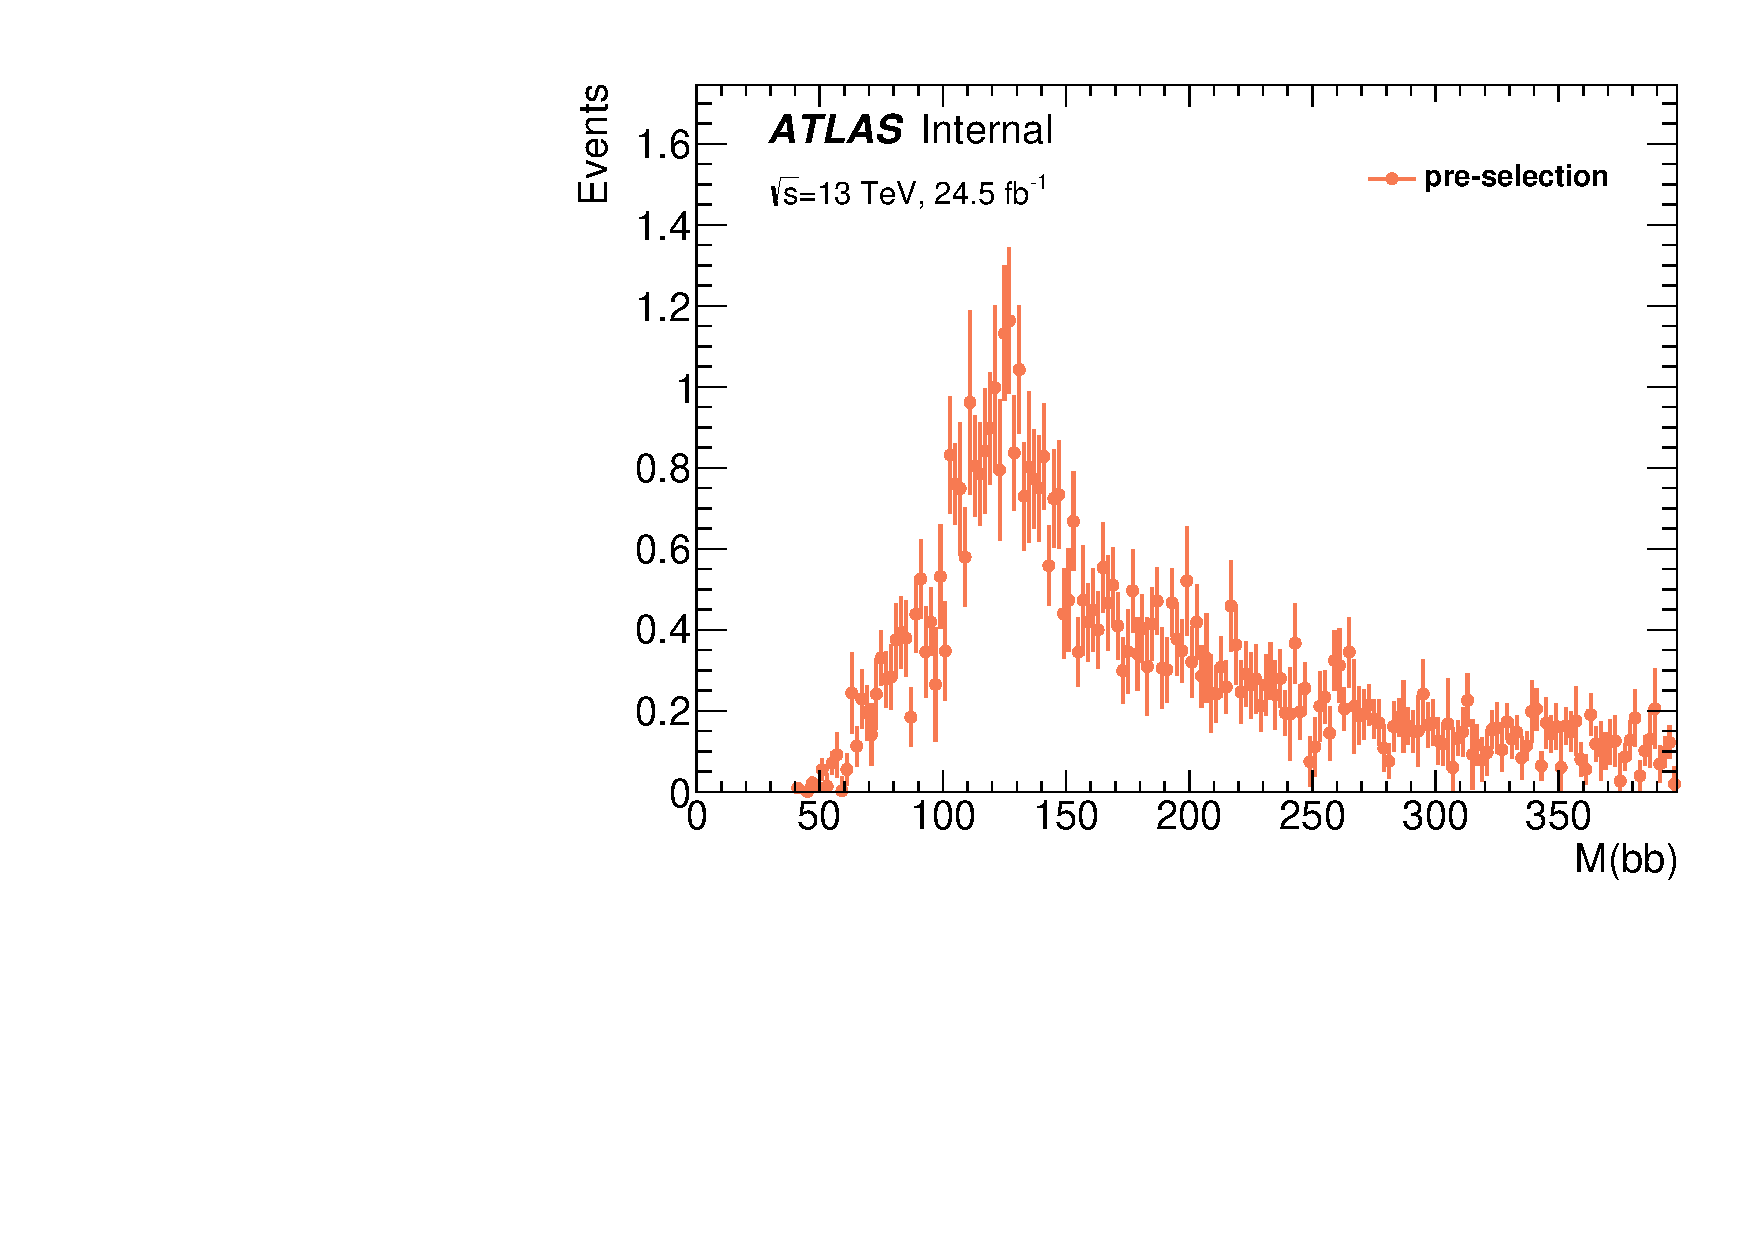
\includegraphics[width=0.42\textwidth]{figures/VBF/Mbb_ttH_2cen.pdf}\\
 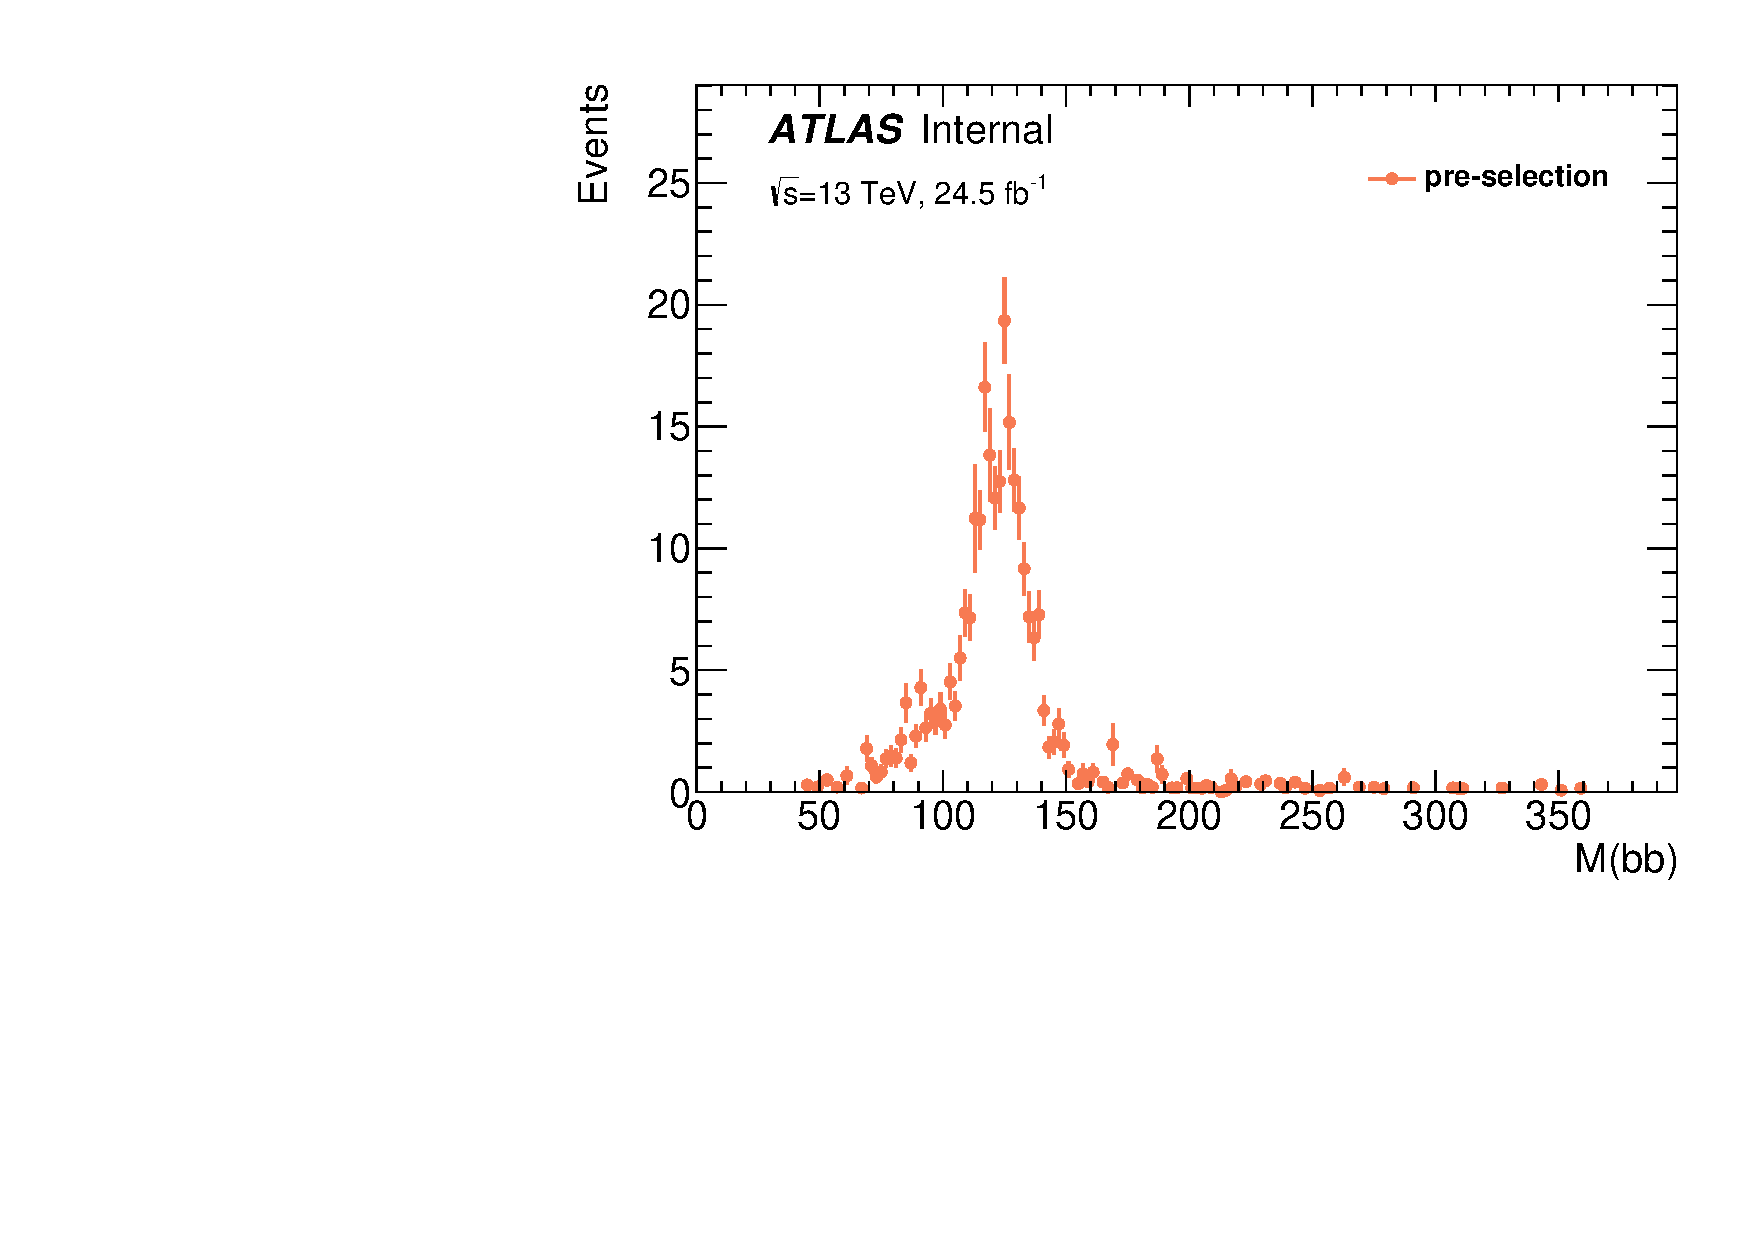
\includegraphics[width=0.42\textwidth]{figures/VBF/Mbb_VH_4cen.pdf}
 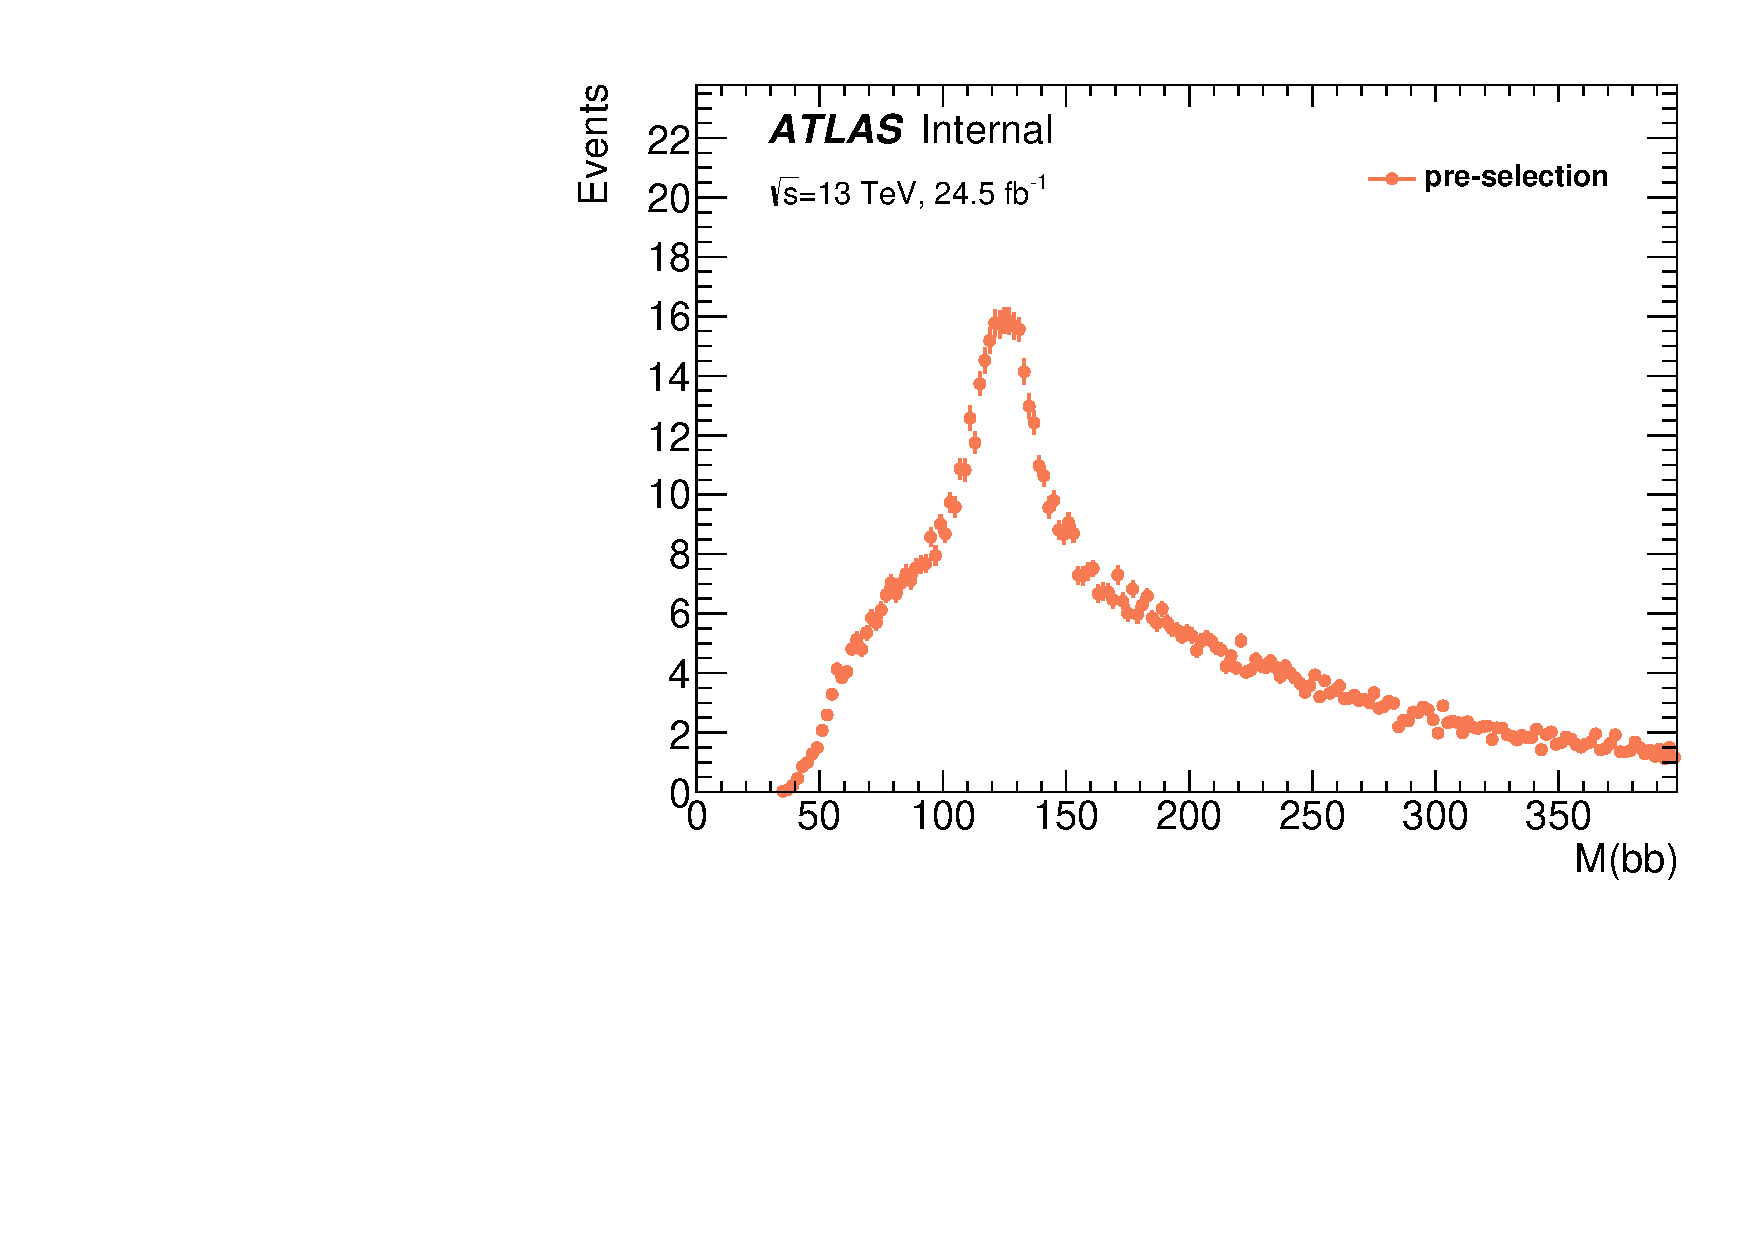
\includegraphics[width=0.42\textwidth]{figures/VBF/Mbb_ttH_4cen.pdf}
 \caption{\Mbb distributions of \VH (left) and \ttH (right) for \twocentral (top) and \fourcentral (bottom) channels passing event pre-selection. }
  \label{fig:Mbb-ttH-VH}
\end{figure}

\begin{table}[htbp]
\centering
\caption{Yields of \VH and \ttH}
\label{tab:vh-tth-yield}
\begin{tabular}{|l|l|l|l|l|}
\hline
     & \multicolumn{2}{l|}{\twocentral SR I}    & \multicolumn{2}{l|}{\twocentral SR II}  \\ \hline
     & Expected Yied  & Fraction of Total Yield & Expected Yied & Fraction of Total Yield \\ \hline
\VH  & 0.2           & 0.2\%                  & 9.3          & 6.8\%                  \\ \hline
\ttH & 4.2           & 2.9\%                  & 30.0         & 19.7\%                 \\ \hline
     & \multicolumn{2}{l|}{\fourcentral SR I}   & \multicolumn{2}{l|}{\fourcentral SR II} \\ \hline
     & Expected Yied  & Fraction of Total Yield & Expected Yied & Fraction of Total Yield \\ \hline
\VH  & 1.4           & 2.0\%                  & 0.7          & 1.4\%                  \\ \hline
\ttH & 0.6           & 0.8\%                  & 2.2          & 4.2\%                  \\ \hline
     & \multicolumn{2}{l|}{\fourcentral SR III} & \multicolumn{2}{l|}{\fourcentral SR IV} \\ \hline
     & Expected Yied  & Fraction of Total Yield & Expected Yied & Fraction of Total Yield \\ \hline
\VH  & 6.0           & 5.2\%                  & 34.1         & 13.5\%                  \\ \hline
\ttH & 12.4          & 10.2\%                 & 42.4         & 15.5\%                 \\ \hline
\end{tabular}
\end{table}

\clearpage

\subsubsection{Summary}
The typical signal yield changes due to a few representative systematic uncertainties are 
shown in Tables. \ref{tab:syst-2cen} and \ref{tab:syst-4cen}.  The theory uncertainties, especially from the QCD scale dominate, at the 20\% level across all signal regions.  The largest experimental uncertainties are from \btagging, at the 3--4\% level.

\begin{table}[hbpt]
\centering
\scriptsize
\begin{tabular}{|l|l|l|l|l|l|l|}
\hline
                 & \multicolumn{6}{c|}{\twocentral}                     \\ \hline
                 & \multicolumn{3}{c|}{SRI} & \multicolumn{3}{c|}{SRII} \\ \hline
                 & Total  & VBF    & ggF    & Total   & VBF    & ggF    \\ \hline
Jet Energy Scale NP1           & 0.75   & 1.19   & 1.14   & 2.54    & 4.11   & 2.07   \\ \hline
Jet Energy Scale \bjets        & 1.52   & 1.62   & 1.08   & 2.21    & 2.71   & 2.06   \\ \hline
Jet Energy Resolution          & 1.65   & 3.03   & 4.11   & 2.16    & 4.69   & 4.19   \\ \hline
\qgtagging                     & 0.65   & 0.73   & 0.28   & 1.39    & 2.12   & 1.18   \\ \hline
Pile-up Reweighting            & 0.49   & 0.18   & 1.74   & 0.18    & 0.99   & 0.54   \\ \hline
\btagging NP0 70WP             & 2.66   & 2.67   & 2.60   & 2.88    & 2.74   & 2.92   \\ \hline
\btagging NP0 85WP             & 0.80   & 0.87   & 0.52   & 1.26    & 1.08   & 1.31   \\ \hline
$\alpha_s$                     & 0.73   & 0.14   & 3.18   & 2.66    & 3.95   & 3.35   \\ \hline
QCD scale VBF                  & 9.92   & 12.29  & 0      & 2.41    & 10.50  & 0      \\ \hline
QCD scale ggF                  & 8.17   & 0      & 42.33  & 29.61   & 0      & 41.91  \\ \hline
PDF Variations                 & 10.08  & 11.52  & 4.16   & 6.36    & 9.56   & 5.42   \\ \hline
Parton Shower                  & 0.34   & 1.06   & 2.69   & 0.62    & 1.92   & 0.24   \\ \hline
\end{tabular}
\caption{Yield change in percentage due to $\pm 1 \sigma$ variation of systematics for \twocentral for combined signal, VBF and ggF production modes. }
\label{tab:syst-2cen}
\end{table}


\begin{table}[hbpt]
\centering
\scriptsize
\begin{tabular}{|l|l|l|l|l|l|l|l|l|l|l|l|l|}
\hline
                    & \multicolumn{12}{c|}{\fourcentral}                                                                                \\ \hline
                    & \multicolumn{3}{c|}{SR I} & \multicolumn{3}{c|}{SR II} & \multicolumn{3}{c|}{SR III} & \multicolumn{3}{c|}{SR IV} \\ \hline
                    & Total   & VBF    & ggF    & Total   & VBF     & ggF    & Total   & VBF     & ggF     & Total   & VBF     & ggF    \\ \hline
Jet Energy Scale NP1      & 3.38    & 1.05   & 18.50  & 0.65    & 0.57    & 3.10   & 1.56    & 2.43    & 0.76    & 1.12    & 0.59    & 1.44   \\ \hline
Jet Energy Scale \bjets   & 0.21    & 0.64   & 1.67   & 1.48    & 1.57    & 12.9   & 0.49    & 1.35    & 0.31    & 1.66    & 2.25    & 1.46   \\ \hline
Jet Energy Resolution     & 1.16    & 1.25   & 12.04  & 0.35    & 2.20    & 3.38   & 3.96    & 1.14    & 8.64    & 1.13    & 0.79    & 1.78   \\ \hline
\qgtagging                & 3.98    & 2.41   & 10.69  & 0.21    & 0.60    & 1.86   & 0.33    & 1.81    & 0.22    & 0.11    & 4.27    & 1.56   \\ \hline
Pile-up Reweighting       & 0.34    & 0.38   & 0.17   & 2.17    & 2.06    & 4.19   & 1.49    & 0.19    & 3.04    & 2.55    & 2.23    & 2.66   \\ \hline
\btagging NP0 77WP        & 4.37    & 4.33   & 4.53   & 4.19    & 4.17    & 4.23   & 4.30    & 4.12    & 4.47    & 4.21    & 4.15    & 4.25   \\ \hline
$\alpha_s$                & 0.76    & 0.16   & 3.35   & 1.32    & 0.23    & 3.45   & 1.85    & 0.34    & 3.23    & 2.85    & 0.90    & 3.49   \\ \hline
QCD scale VBF             & 6.69    & 8.25   & 0      & 5.39    & 8.06    & 0      & 3.86    & 8.08    & 0       & 1.98    & 7.95    & 0      \\ \hline
QCD scale ggF             & 7.83    & 0      & 41.56  & 12.86   & 0       & 40.66  & 22.67   & 0       & 43.42   & 31.99   & 0       & 42.60  \\ \hline
PDF Variations            & 6.19    & 6.44   & 5.16   & 5.62    & 6.33    & 4.18   & 5.03    & 6.11    & 4.05    & 4.95    & 7.23    & 4.19   \\ \hline
Parton Shower             & 3.24    & 4.14   & 0.62   & 1.75    & 3.56    & 1.87   & 2.36    & 0.31    & 0.96    & 0.26    & 0.32    & 0.24   \\ \hline
\end{tabular}
\caption{Yield change in percentage due to $\pm 1 \sigma$ variation of systematics for \fourcentral for combined signal, VBF and ggF production modes.}
\label{tab:syst-4cen}

\end{table}




\subsection{Profile Likelihood and yield determination}

The negative log-likelihood is constructed as shown in Eq.\ref{likelihood-old}, 
where $Y_{ijk}$ denotes the yield of $k^{th}$ bin of $j^{th}$ region of $i^{th}$ channel. 
Nuisance parameters, which have external constraints $f(\alpha_l)$, are penalized in the negative log-likelihood. 
b
The  \fourcentral{} channel consists of two signal regions and its corresponding control region, while the \twocentral{} channel consists of three signal regions and its control region,
for a total of seven \Mbb{} distributions.
The yield of each region is calculated with Eq.\ref{yield-old}.
Note that the yields of signal regions and control regions are calculated differently
following the assumption that signal contributions in the control regions are negligible. 

The control regions are used to constrain the background shape as well as to determine 
the bias introduced by the functional form chosen to describe the background ($\mu_{sp}$).
To propagate the uncertainty of the spurious signal and correct its impact on the signal strength, 
the spurious signal is a free parameter in the profile likelihood.
Other free parameters are the normalizations of the non-resonant background in each control and
signal region, denoted with $N_B$.
The signal normalizations $N_H$ are set to the Standard Model expectation from simulation,
while $\mu$ represents the observed signal strength.
The shapes of Higgs, Z and non-resonant background are $H$, $Z$ and $B$, respectively.
The linear correction for the background parameterization across signal and control regions is denoted with $T$. 

\begin{equation}
\label{likelihood-old}
-\log\mathcal{L}(\mu, \{\alpha_{l}\} )= -\log \prod_{i=1}^{\textnormal{Channels}} \prod_{j=1}^{\textnormal{Regions}} \prod_{k=1}^{\textnormal{Bins}} \frac{e^{-Y_{ijk}(\mu, \{\alpha_l\})} \times Y_{ijk}N_{ijk}^{Obs} }{N_{ijk}^{Obs}} - \log \prod_{l}^{\textnormal{Nuisance Pars}} f(\alpha_l)
\end{equation}

\begin{equation}
\label{yield-old}
\begin{split}
Y_{CR} &= \mu N_{H}(CR)H(CR)+  \mu_{sp}\hat{N}_{H}H(SRI) \\
       &+ N_{B}(CR)B+ \alpha_{z}(Norm)\alpha_{z}(CR)N_{Z}(CR)Z  \\
Y_{SRI} &= (\mu+\mu_{sp})N_{H}(SRI)H(SRI) \\
        &+ N_{B}(SRI)BT(CR\rightarrow SRI) + \alpha_{z}(Norm)\alpha_{z}(SRI)N_{Z}(SRI)Z\\
Y_{SRII} &= (\mu+\mu_{sp}\frac{N_{B}(SRII)}{N_{B}(SRI)})N_{H}(SRII)H(SRII) \\
         & + N_{B}(SRII)BT(CR\rightarrow SRII) + \alpha_{z}(Norm)\alpha_{z}(SRII)N_{Z}(SRII)Z \\
Y_{SRIII} &= (\mu+\mu_{sp}\frac{N_{B}(SRIII)}{N_{B}(SRI)})N_{H}(SRIII)H(SRIII) \\
          & + N_{B}(SRIII)BT(CR\rightarrow SRIII) + \alpha_{z}(Norm)\alpha_{z}(SRIII)N_{Z}(SRIII)Z\\
\hat{N}_H &= N_B(CR)/N_B(SRI)\times N_{H}(SRI)
\end{split}
\end{equation}

The nuisance parameter $\alpha_{z}$ controls the overall normalization for the \zjets{} template 
and is constrained with a Gaussian prior with width 0.1. The overall normalization is scaled to 0.74 and 0.79 for \twocentral and \fourcentral channels, respectively, determined as described in Section~\ref{sec:ztreat}.
We also adopt independent NPs for each BDT region to account the data/MC shape difference of \zjets{}. 
%The chosen values are motivated by the validation study in data described in Appendix~\ref{sec:zjets}. 


\subsubsection{Fit toy experiments}

To determine if the fit procedure yields bias, we build 1000 toy experiments from the background function determined in background only fit and inject the \Zjets{} component fixed at the Standard Model prediction. The Higgs signals are injected of different strengths at $\mu_{inj} = 0.5, 1.0, 2.0, 5.0$. The pulls of the toy experiment fits defined as $(\mu_{fit}-\mu_{inj})/ \sigma$ are shown in Figures \ref{fig:MCToy-old}. The distributions of pulls are fitted with Gaussian distribution to determine means and widths, which are consistent with 0 and 1 within statistical uncertainties. For $\mu_{inj}=1.0$ test, we fit back $\hat{\mu}=1.00\pm 1.14$. The expected signal significance in this case is 0.87. The asymptotic Asimov fit for $\mu_{inj}=1.0$ is shown in Fig. \ref{fig:Asimov-old}


\begin{figure}[htbp]
  \centering
 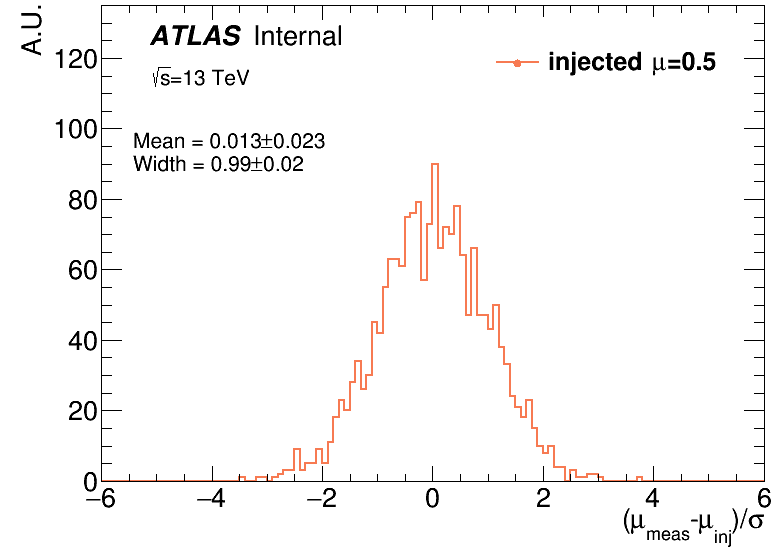
\includegraphics[width=0.45\textwidth]{figures/FitCombined/mu05.PNG}
 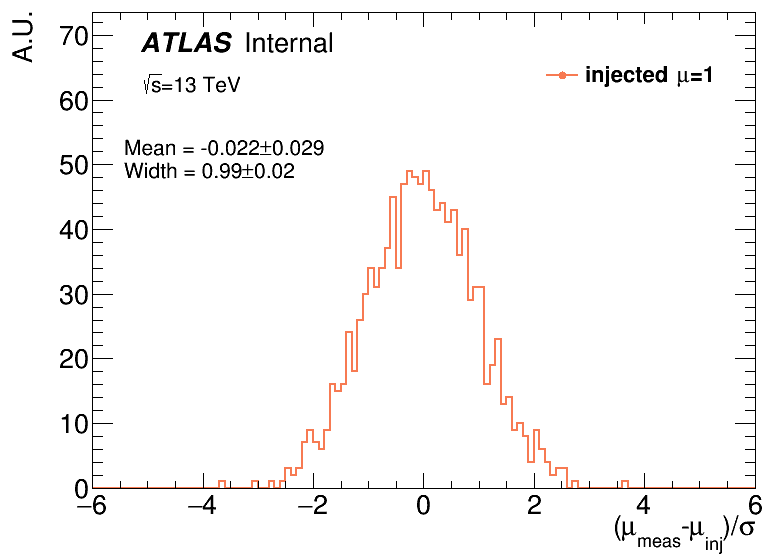
\includegraphics[width=0.45\textwidth]{figures/FitCombined/mu1.PNG}\\
 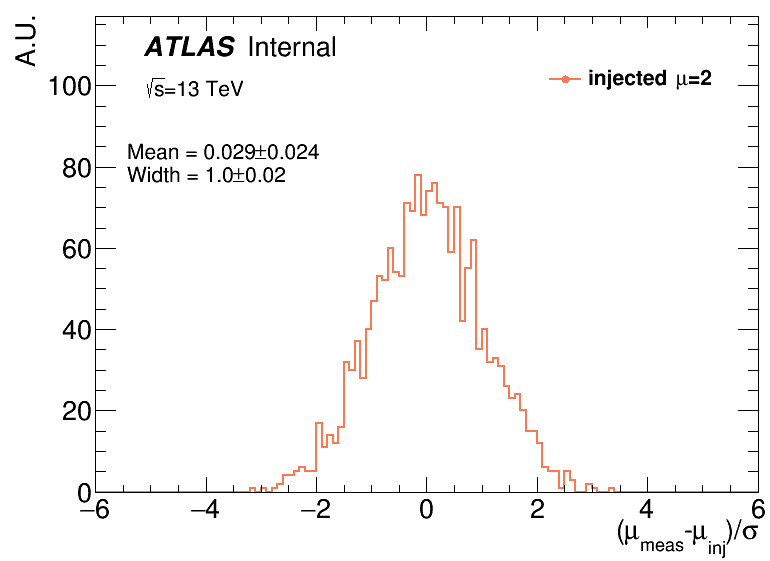
\includegraphics[width=0.45\textwidth]{figures/FitCombined/mu2.PNG}
 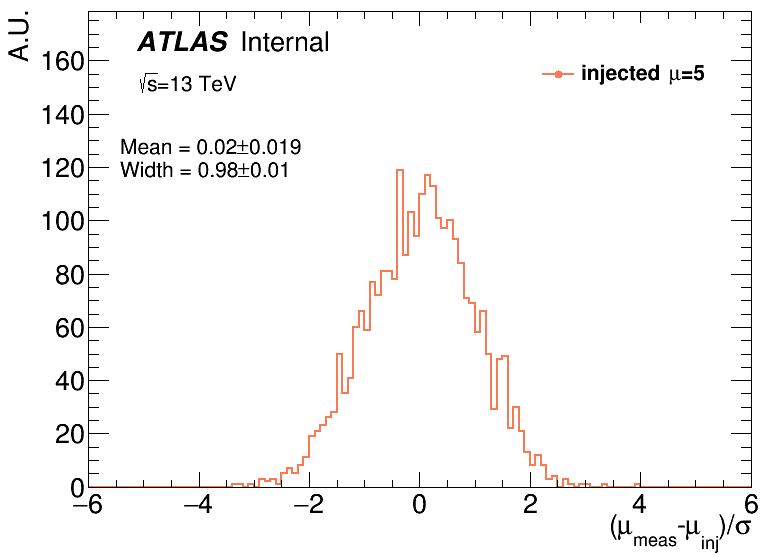
\includegraphics[width=0.45\textwidth]{figures/FitCombined/mu5.PNG}\\
\caption{Pull distribution of toy experiment fits. We inject Higgs signal strength of 0.5 (top left), 1.0 (top right), 2.0 (bottom left) and 5.0 (bottom right) times the Standard Model prediction. The pulls are fitted with Gaussian to determine the means and widths which are unbiased. }
  \label{fig:MCToy-old}
\end{figure}


\begin{figure}[htbp]
  \centering
 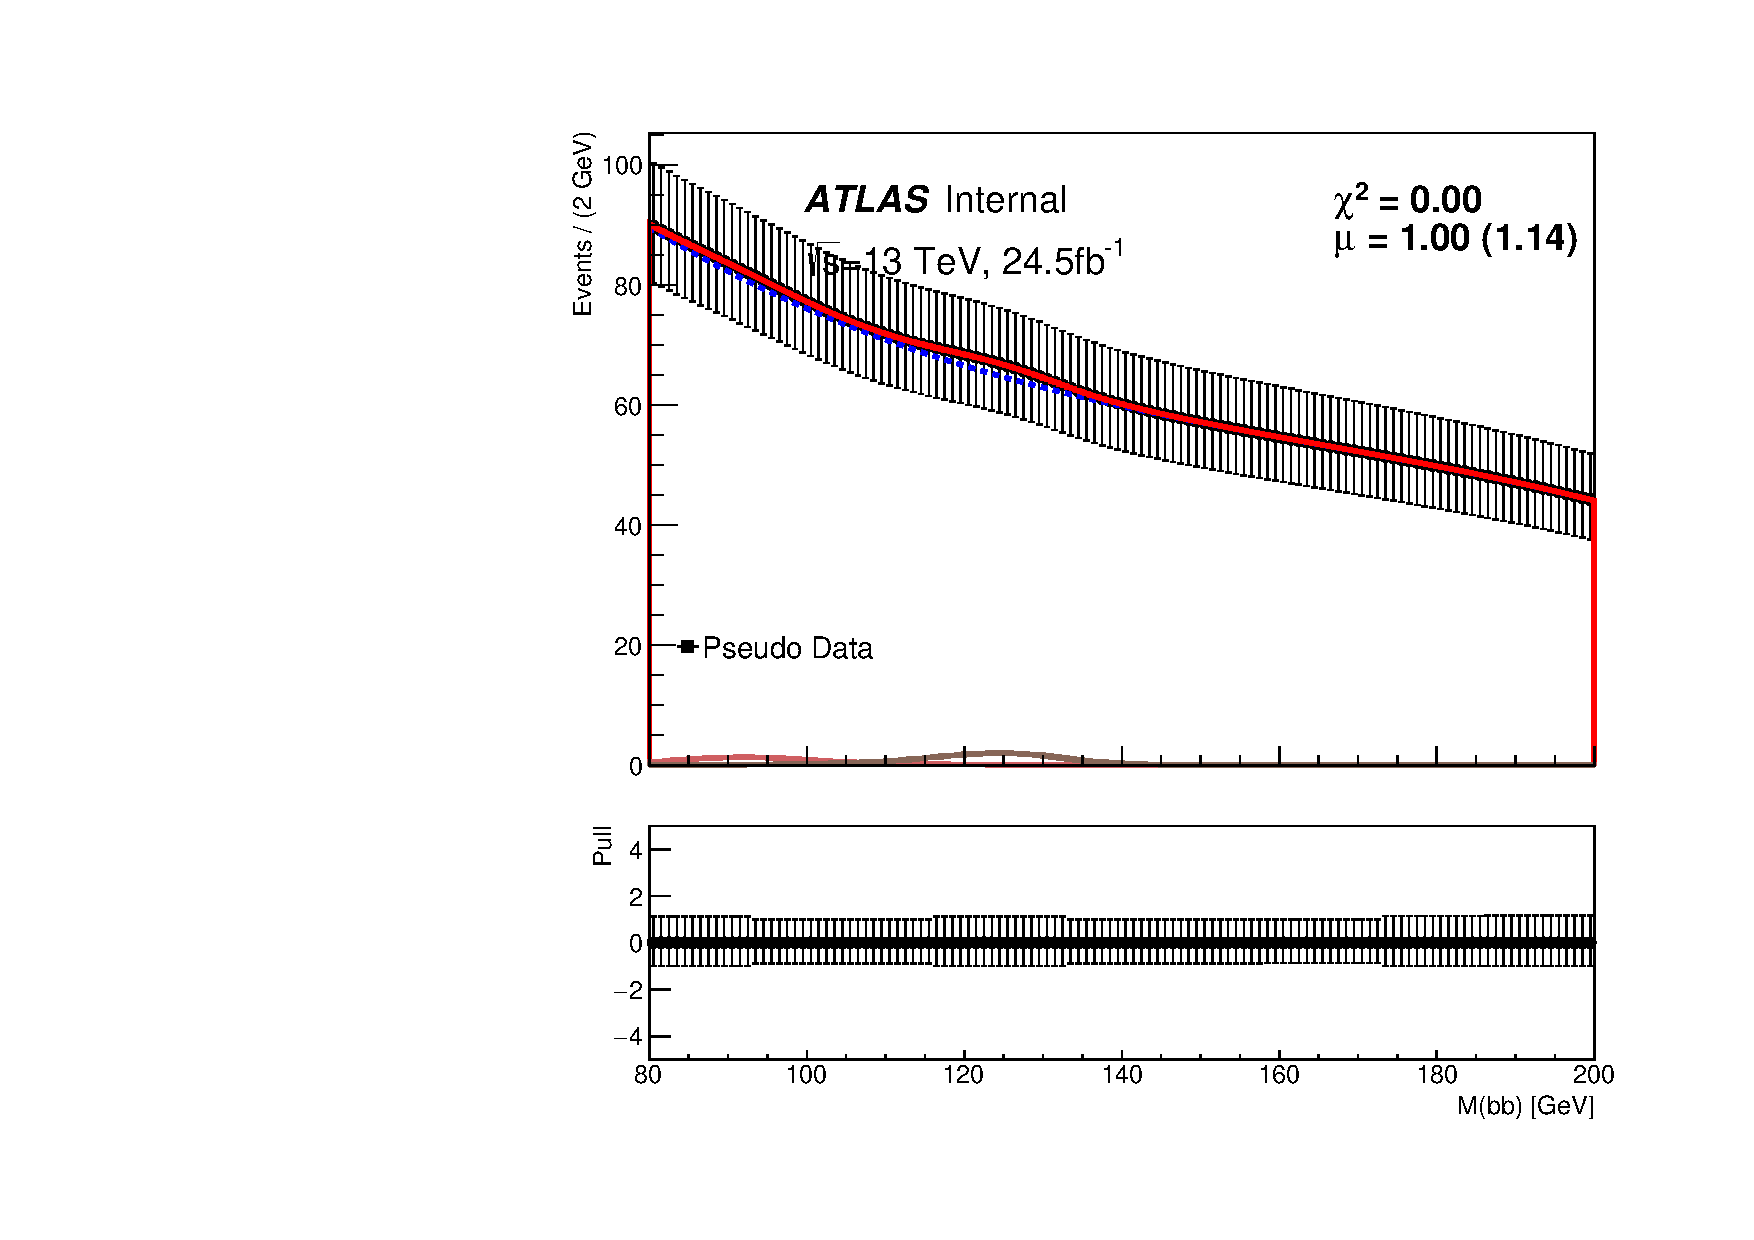
\includegraphics[width=0.32\textwidth]{figures/FitCombined/Asimov_testVBF_ICHEP_2cen_SRI.pdf}
 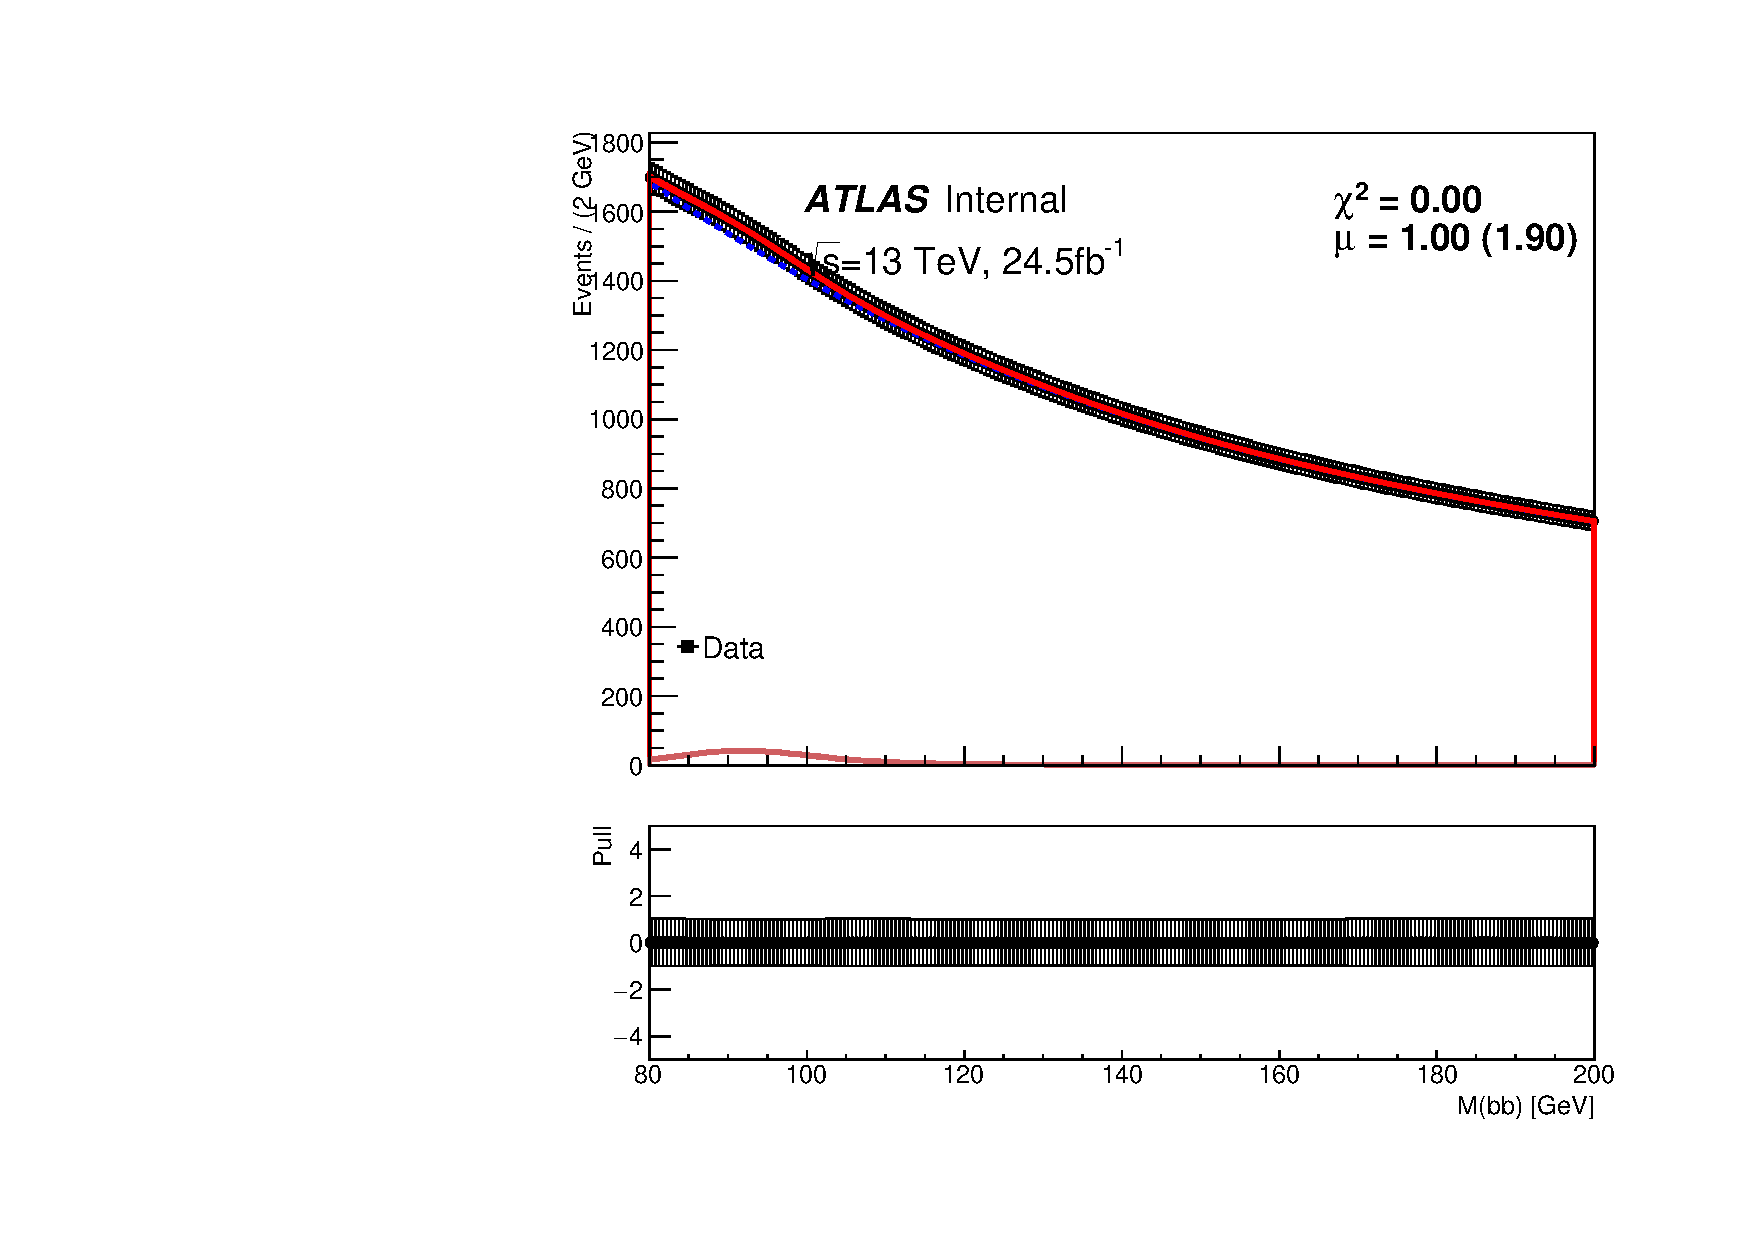
\includegraphics[width=0.32\textwidth]{figures/FitCombined/Asimov_testVBF_ICHEP_2cen_SRII.pdf}
 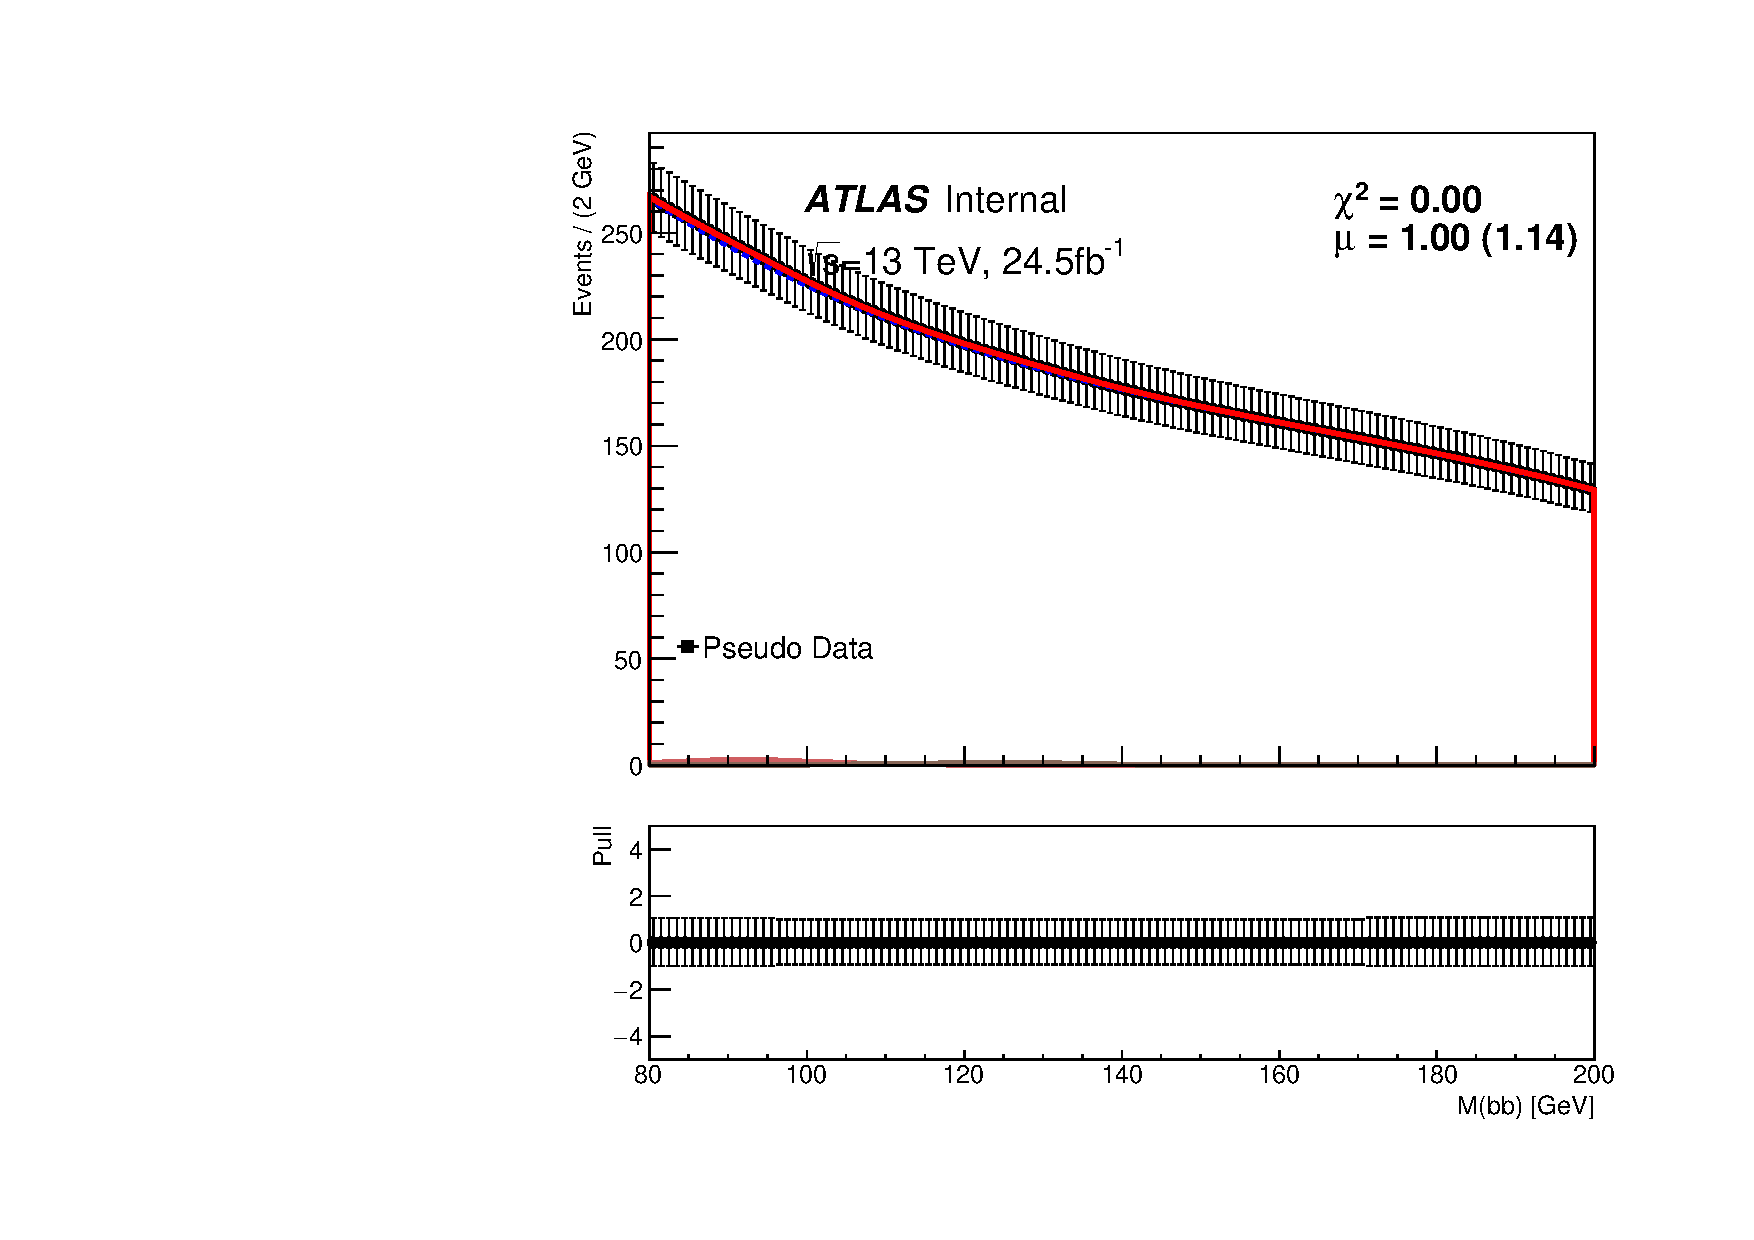
\includegraphics[width=0.32\textwidth]{figures/FitCombined/Asimov_testVBF_ICHEP_2cen_SRIII.pdf}\\
 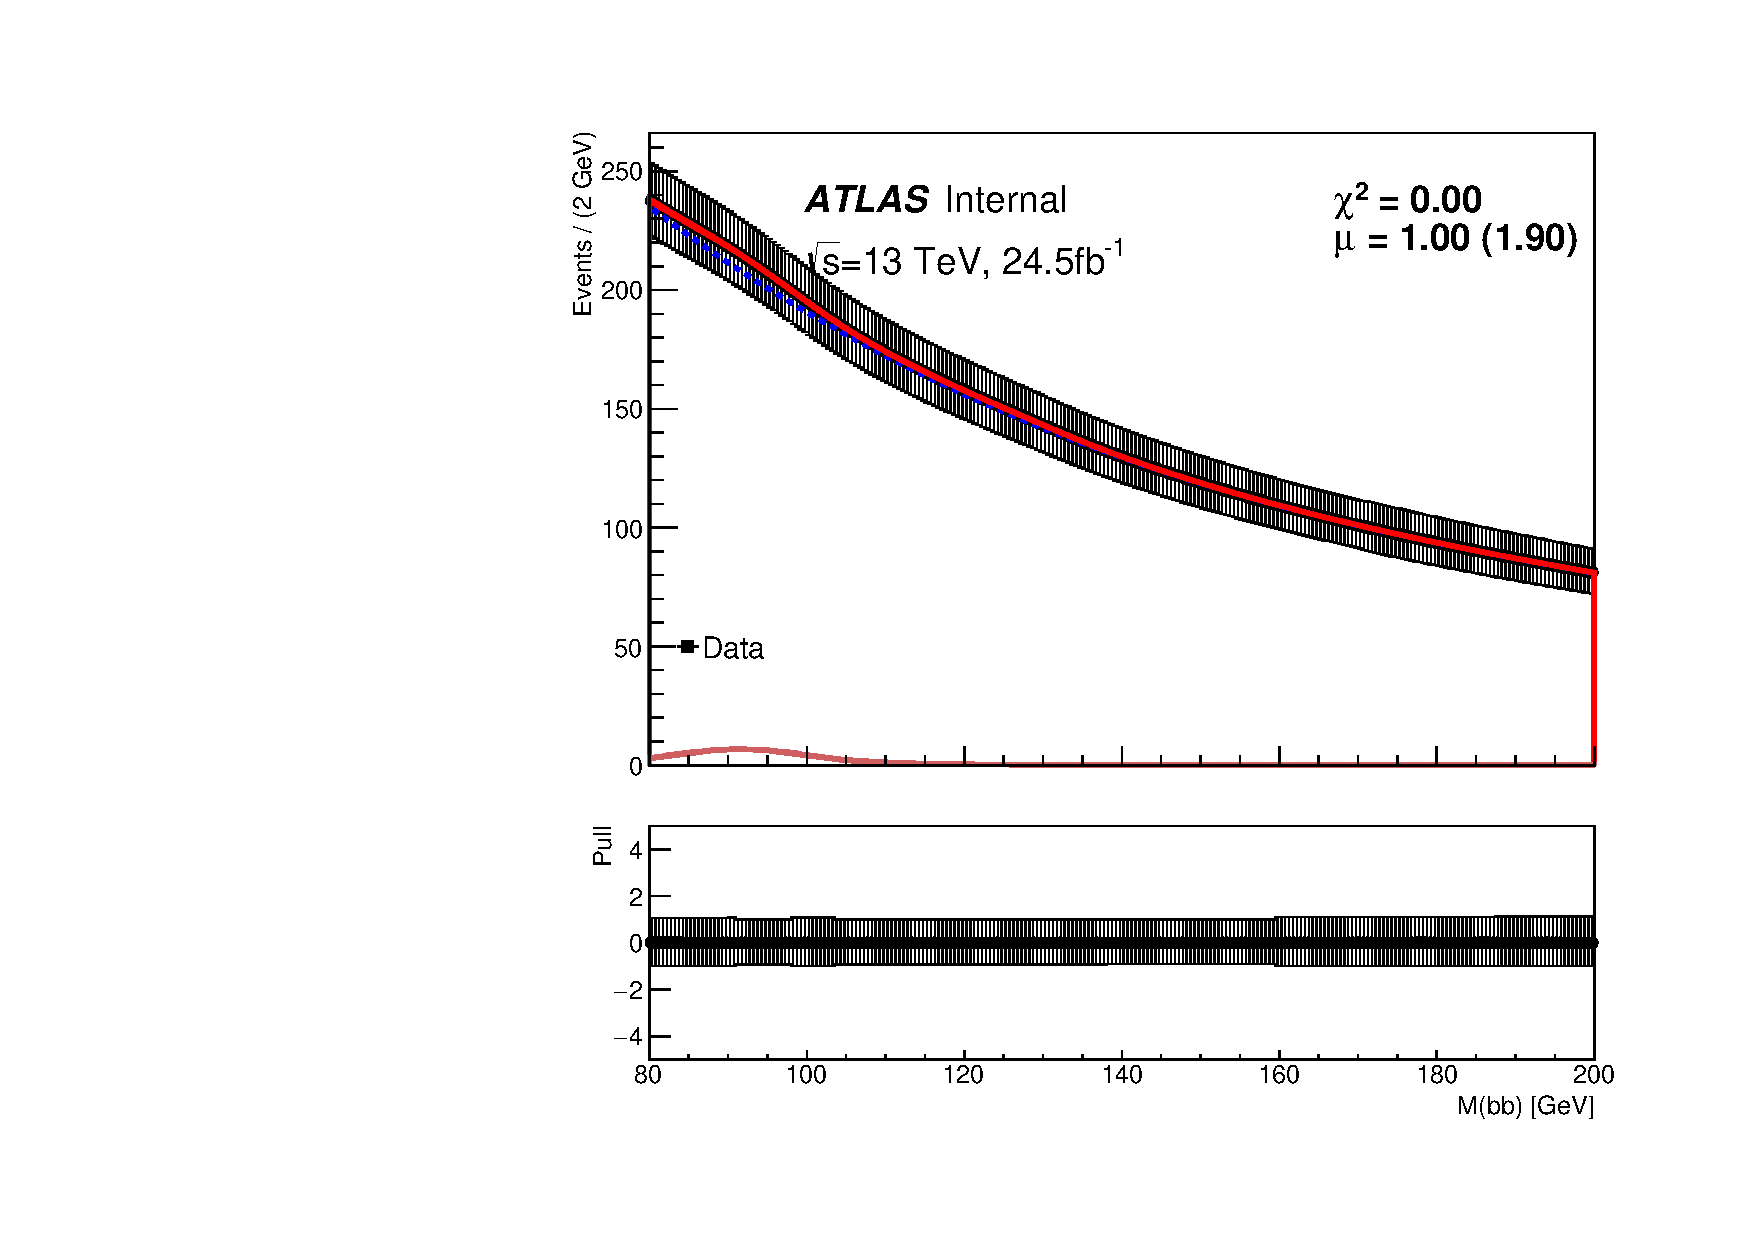
\includegraphics[width=0.32\textwidth]{figures/FitCombined/Asimov_testVBF_ICHEP_4cen_SRI.pdf}
 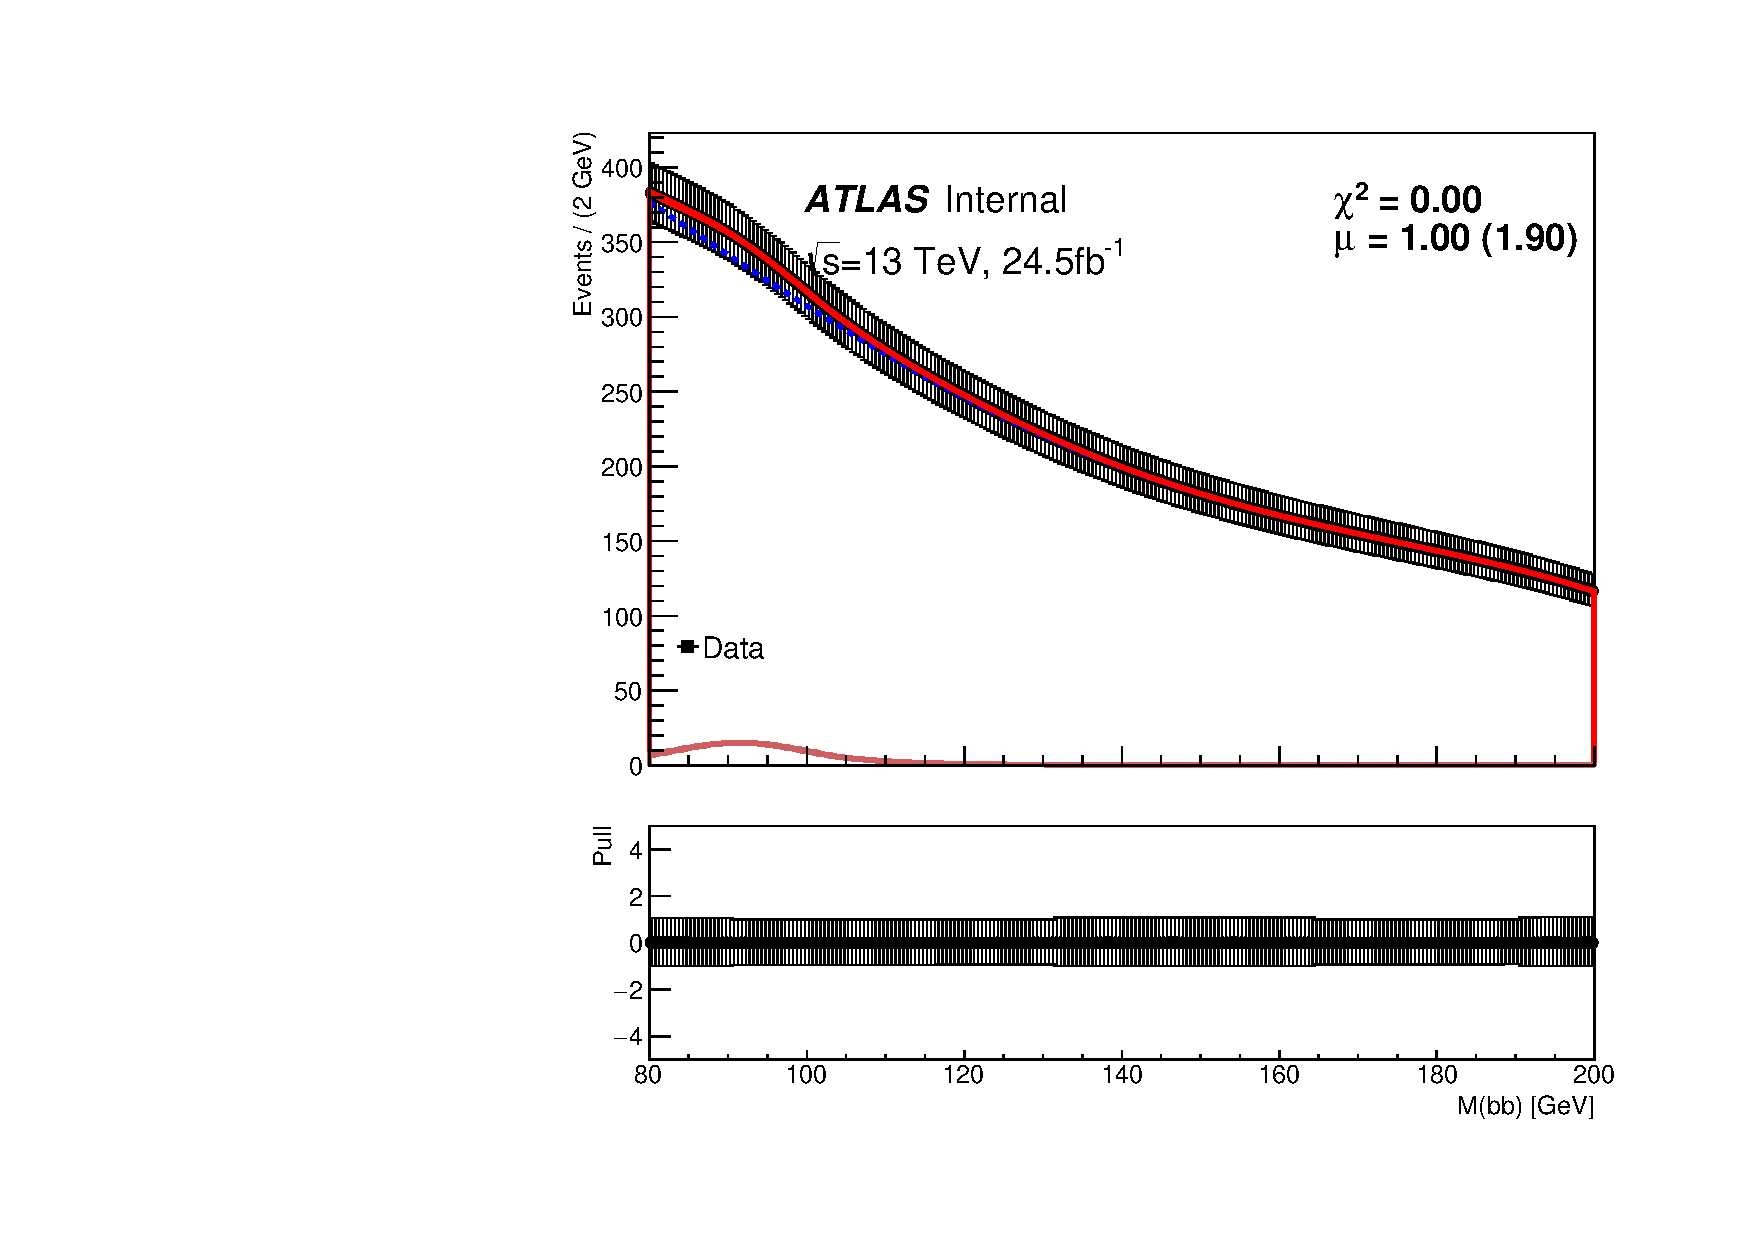
\includegraphics[width=0.32\textwidth]{figures/FitCombined/Asimov_testVBF_ICHEP_4cen_SRII.pdf}\\

\caption{Asymptotic Asimov fit for both channels. Fits from SR I to SR III (SR II) for 2 central (top) and 4 central (bottom) are shown.}
  \label{fig:Asimov-old}
\end{figure}


\subsubsection{Fit pseudo-data}

Another check to test the robustness of the fit method as well as a check of the nuisance parameter pulls 
is to use pseudo-data as close as possible to the real data. 
For each signal region we construct the pseudo data by adding together three components:
\begin{enumerate}
\item Sideband ($80~\GeV <\Mbb<100$~\GeV~and $140~\GeV<\Mbb<200~\GeV$)
\item Control region data in the Higgs mass window re-weighted linearly to the signal region using the fits described in Section~\ref{sec:nonres-old}.
\item Signal MC scaled to Standard Model expectation for Higgs and \zjets{} production.
\end{enumerate}

The fit is performed simultaneously with both channels. We obtain closure as the best fitted signal strength is $\hat \mu = 0.56 \pm 1.15$. The fits are shown in Figures~\ref{fig:Fit_combined-old}. The post-fit impact of nuisance parameters and pulls for the simultaneous fit are shown in Figure~\ref{fig:pull-old}.  
The parameters are defined as:
\begin{itemize}
\item nbkg\_X\_Y stands for background normalization in region X channel Y
\item spurious stands for the strength of spurious signal
OB\item  Lin\_X\_Y stands for the linear slope correction in region X channel Y
\item x()2cen, x()4cen stands for Bernstein polynomial parameters in the \twocentral and \fourcentral channels respectively
\item $\alpha\_z$ stands for the Z normalization NP
\end{itemize} 
The other parameter names follow the CP group definitions.  
The largest contributions to the uncertainty on $\mu$ are from the background normalization and 
control to signal region linear transfer factors. 
%The only parameter pulled significantly is the $Z$ normalization, 
%which is expected as we use a leading order generator for our $Z$+jets contribution.  
%Further studies of the $Z$-contribution are discussed in Section~\ref{sec:znorm}.  

\begin{figure}[htbp]
  \centering
 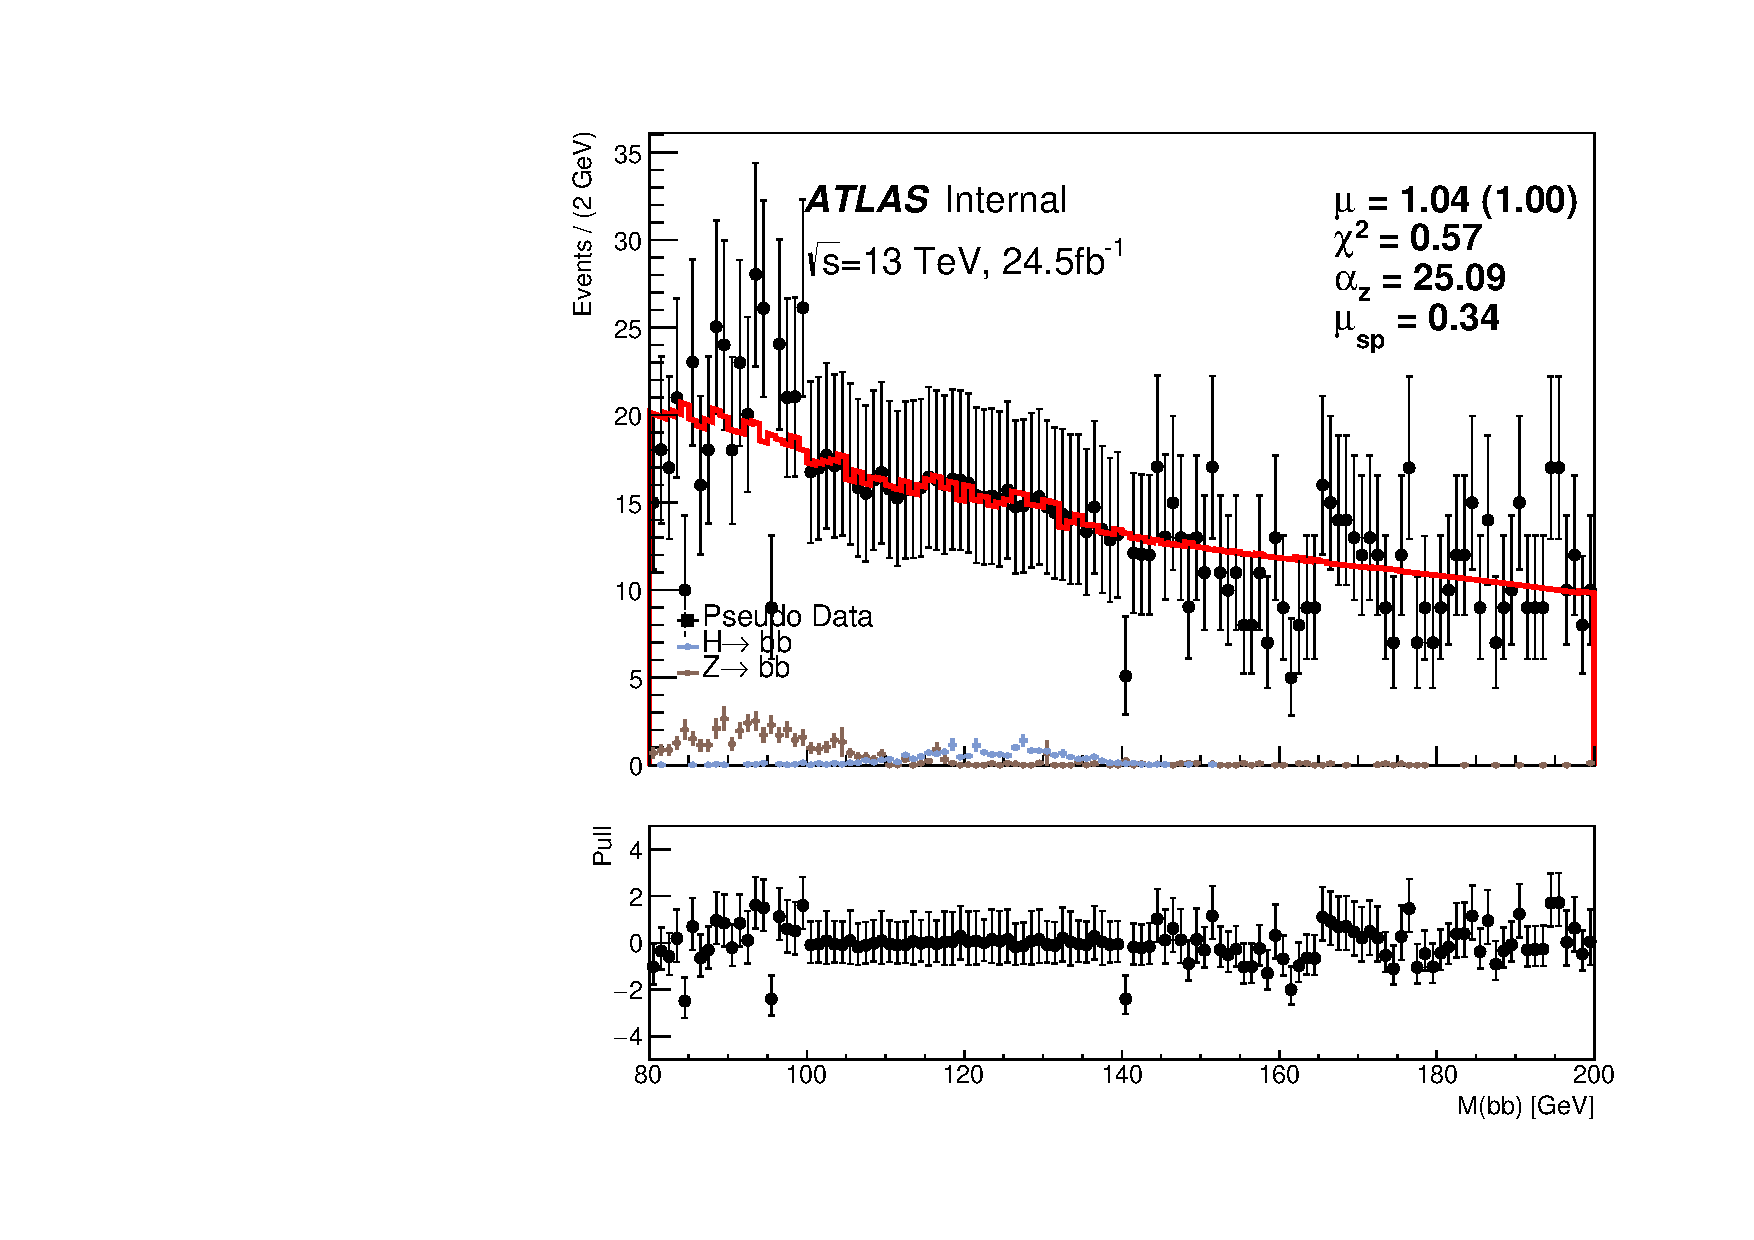
\includegraphics[width=0.32\textwidth]{figures/FitCombined/zcon_testVBF_ICHEP_2cen_SRI.pdf}
 \includegraphics[width=0.32\textwidth]{figures/FitCombined/zcon_testVBF_ICHEP_2cen_SRII.pdf}
 \includegraphics[width=0.32\textwidth]{figures/FitCombined/zcon_testVBF_ICHEP_2cen_SRIII.pdf}\\
 \includegraphics[width=0.32\textwidth]{figures/FitCombined/zcon_testVBF_ICHEP_4cen_SRI.pdf}
 \includegraphics[width=0.32\textwidth]{figures/FitCombined/zcon_testVBF_ICHEP_4cen_SRII.pdf}\\

\caption{Pseudo data fit for both channels. Fits from SR I to SR III (SR II) for 2 central (top) and 4 central (bottom) are shown.}
  \label{fig:Fit_combined-old}
\end{figure}


%\begin{figure}[htbp]
 % \centering
 %\includegraphics[width=0.5\textwidth]{figures/PseudoDataToys.pdf}
%\caption{Fitted signal strength of pseudo data toys.}
%  \label{fig:PseudoToy}
%\end{figure}


\begin{figure}[htbp]
  \centering
 \includegraphics[width=0.9\textwidth]{figures/FitCombined/VBFHbb_pulls_125_Asimov.pdf}

\caption{Nuisance parameter post-fit impact and pulls are plotted for the simultaneous Asimov fit of two channels. The background normalizations are pre-fixed as "nbkg''. The Linear transfer function are pre-fixed as "Lin''. The spurious signal size are pre-fixed as "spurious''. The background parameterizations are pre-fixed as  "x()2cen'' for 2 central channel and "x()4cen'' for 4 central channel. The JES and JER parameters are prefixed by ``alpha\_ATLAS\_JET".  The \btagging parameters are prefixed by ``alpha\_ATLAS\_eigen". The most significant contribution to the uncertainty of signal strength comes from background normalization.}
  \label{fig:pull_asimov-old}
\end{figure}


\begin{figure}[htbp]
  \centering
 \includegraphics[width=0.95\textwidth]{figures/FitCombined/Correlation.pdf}

\caption{Nuisance parameter correlation for Asimov fit}
  \label{fig:corr_asimov-old}
\end{figure}




\begin{figure}[htbp]
  \centering
 \includegraphics[width=0.9\textwidth]{figures/FitCombined/VBFHbb_pulls_125.pdf}

\caption{Nuisance parameter post-fit impact and pulls are plotted for the simultaneous fit of two channels for the pseudodata. The background normalizations are pre-fixed as "nbkg''. The Linear transfer function are pre-fixed as "Lin''. The spurious signal size are pre-fixed as "spurious''. The background parameterizations are pre-fixed as  "x()2cen'' for 2 central channel and "x()4cen'' for 4 central channel. The JES and JER parameters are prefixed by ``alpha\_ATLAS\_JET".  The \btagging parameters are prefixed by ``alpha\_ATLAS\_eigen". The most significant contribution to the uncertainty of signal strength comes from background normalization.}
  \label{fig:pull-old}
\end{figure}
